\chapter{The Photaura spectral model}
\label{ch:photaura}

Photaura is spectral model for high temperature gases that can presently treat bound-bound transitions of monatomic and diatomic species in a line-by-line manner and monatomic continuum processes via hydrogenic approximations or tabulated cross-sections.
The \texttt{photaura} model is described and implemented in the PhD thesis of Potter~\cite{Potter_PhD} where good agreement with air and CO$_2$--N$_2$ shock tube spectroscopy measurements in the NASA Ames EAST facility was found.  
The \texttt{photaura} model was also found by Sobbia et al~\cite{SLB+2013} to accurately reproduce intensity spectra measured in an ICP facility with a N$_2$--CH$_4$ test gas.
This chapter is comprised on two sections; spectral modelling in \textsection~\ref{sec:spec_rad}, and collisional-radiative modelling in \textsection~\ref{sec:CR}.

\section{Spectral radiation coefficients}
\label{sec:spec_rad}

The calculation of the spectral radiation coefficients, namely the emission $j_\nu$ and absorption $\kappa_\nu$ coefficients, are required when solving the radiation transfer equation presented in Equation~\ref{eq:RTE}.
For an ionised gas, there are three types of radiative mechanisms that make contributions to the bulk spectral coefficients:

\begin{enumerate}
 \item Bound-bound transitions,
 \item Bound-free transitions, and
 \item Free-free transitions.
\end{enumerate}

Bound-bound radiative transitions occur between two bound electronic states, whilst bound-free and free-free radiative transitions involve a free electron state.
Figure~\ref{fig:sample_absorption_spectra} presents a sample vacuum ultraviolet absorption coefficient spectra with the contributions from bound-bound, bound-free and free-free transitions identified.
As bound electronic states are quantised, the spectrum of a bound-bound transition is distributed about a discrete wavelength characterised by the energy gap between the upper and lower states.
In contrast, the energy spectrum of bound-free and free-free radiative transitions are distributed into a continuum due to the arbitrary free electron energy.
The spectrum of bound-free transitions are further characterised by a limiting wavelength corresponding to the ionisation threshold.

\begin{figure}[h]
 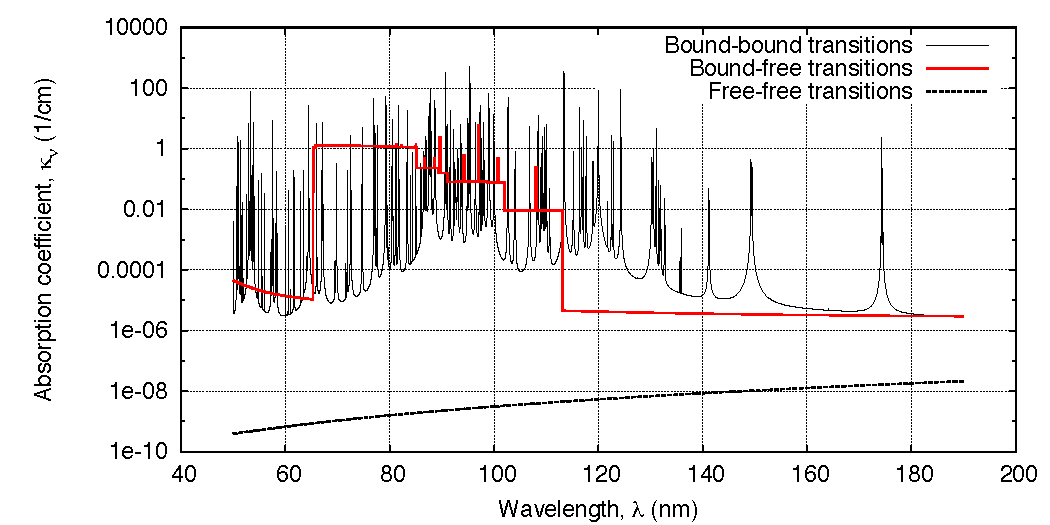
\includegraphics[width=0.9\linewidth]{figures/spectral-modelling/VUV_spectra_components.pdf}
 \caption{Components of the equilibrium vacuum ultraviolet absorption coefficient spectra for a 10\,km/s shock through 0.1\,Torr air.}
 \label{fig:sample_absorption_spectra}
\end{figure}

\par

At the most fundamental level, bound-bound transitions in both atoms and molecules occur between two Zeeman states of a hyperfine line due to the change in nuclear spin.
In the present work bound-bound transitions are described by a line-by-line model that considers the hyperfine structure where necessary.
Continuum transitions are described by step models presented in the literature or hydrogenic approximations when unavailable.
For an indepth discussion of the theory behind the models implemented here, see the texts of Zel'dovich and Razier~\cite{ZR}, Huber and Herzberg~\cite{HH_1979} and Kov\'{a}cs~\cite{kovacs69}.

\subsection{Monatomic bound-bound transitions}
\label{sec:monatomic_transitions}

% state full equations for spectral emission and absorption coefficients here

The spectral emission and absorption coefficients for an atomic or molecular bound-bound transition with energy $h \nu_{u l}$ are:

\begin{equation}
 j_{\nu,ul} = \frac{N_{u} h \nu_{u l} A_{u l}}{4 \pi} b_{ul}(\nu) \text{ , } \label{eq:atomic_j_nu_ul}
\end{equation}

\noindent and,

\begin{equation}
 \kappa_{\nu,lu} = ( N_{l} B_{l u} -N_{u} B_{u l} ) h \nu_{u l} b_{ul}(\nu) \text{ , } \label{eq:atomic_kappa_nu_lu}
\end{equation}

\noindent where $l$ and $u$ denote the lower and upper energy levels, $N$ is the level number density, $A_{ul}$, $B_{lu}$ and $B_{ul}$ are the Einstein coefficients for spontaneous emission, absorption and induced emission, and $b_{ul}(\nu)$ is the spectral distribution function.
The absorption and induced emission $B_{ul}$ Einstein coefficients $B_{lu}$ and $B_{ul}$ can be related to the spontaneous emission Einstein coefficient $A_{ul}$ via the principal of detailed balancing~\cite{ZR}.
Equation~\ref{eq:atomic_kappa_nu_lu} is then expressed as:

\begin{equation}
 \kappa_lu = \left ( N_l \frac{g_u}{g_l} - N_u \right ) \frac{c^2}{8 \pi \nu_{ul}^2} A_{ul} b_{ul}(\nu)
\end{equation}

\subsubsection{Level populations}

For monatomic species, the electronic level populations are bound by two limiting distributions:

\begin{enumerate}
 \item Boltzmann thermal equilibrium distribution, and
 \item Saha-Boltzmann ionisation equilibrium distribution.
\end{enumerate}

At thermal equilibrium conditions the electronic levels are populated according to the Boltzmann distribution, where the number density of level $i$ is expressed as:

\begin{equation}
 N_i = N_\text{atom} \frac{ Q_{\text{el-}i} }{ Q_\text{int-atom} } = N_\text{atom} \frac{g_i \text{~exp} \left ( \frac{-E_i}{kT_\text{el}} \right )}{\sum_j^{j_\text{max}} g_j \text{~exp} \left ( \frac{-E_j}{kT_\text{el}} \right )} \text{ , } \label{eq:atom_boltz}
\end{equation}

\noindent where $N_\text{atom}$ is the total number density of the atom, $E_i$ is the electronic energy of level $i$, $T_\text{el}$ is the electronic temperature and $Q_\text{int-atom}$ is the total internal (electronic) partition function\footnote{Whereas only the first few electronic levels were retained when calculating the partition function for determining thermodynamic properties, all the electronic levels up to the ionisation limit are included for the spectral coefficient calculations.  This is necessary as transitions originating from near the ionisation limit are often very strong, and their populations need to be determined to a high degree of accuracy.}.
Another constraint is imposed by considering chemical equilibrium between the electronic level, ions and free electrons.
The Saha equation relates the number densities of an atom, its ion and free electrons via the principle of detailed balancing:

\begin{equation}
 \frac{ N_\text{atom} }{ N_\text{ion} N_e } = \frac{ Q_\text{atom} }{ Q_\text{ion} Q_e } \text{~exp} \left ( \frac{I_\text{atom}}{k_B T_e} \right ) \text{ , } \label{eq:atom_saha}
\end{equation}

\noindent where $T_e$ is the free electron translation temperature, $Q$ and $N$ are respectively the \textit{total} partition function and total number density of the denoted species  and $I_\text{atom}$ is the ionisation potential of the atom.
By substituting the Boltzmann equation for an electronic level, Equation~\ref{eq:atom_boltz}, into the Saha equation for an atomic species, Equation~\ref{eq:atom_saha}, the Saha-Boltzmann equation is obtained:

\begin{equation}
 N_i =  N_\text{ion} N_e \frac{ Q_\text{atom} }{ Q_\text{ion} Q_e }  \text{~exp} \left ( \frac{I_\text{atom}}{k_B T_e} \right ) \frac{ g_i \text{~exp} \left ( \frac{-E_i}{kT_\text{el}} \right ) }{ Q_\text{int-atom } } \label{eq:atom_saha}
\end{equation} 

In compression flows, the Saha-Boltzmann distribution forms the lower bound and the Boltzmann distribution the upper bound, whilst in expanding flows they are reversed.
As thermochemical equilibration occurs, the atom number density approaches that predicted by the Saha equation and the Saha-Boltzmann and Boltzmann distributions converge to the same result.

\par

To model the level populations in nonequilibrium, the rate of all transitions affecting the level must be considered.
As all transitions can be grouped into those occurring due to particle collisions and those due to radiative transitions, the nonequilibrium modelling of quantum levels is often referred to as `collisional-radiative modelling'.
In the present work we consider the electronic levels of neutral atoms to possess nonequilibrium populations, whilst the electronic levels of atomic ions are assumed to in Boltzmann equilibrium.
The collisional-radiative framework is described in Section~\ref{sec:CR}.

\subsubsection{Electronic level energies and degeneracies}

The critical data for calculating monatomic partition functions are the energies and degeneracies of the electronic levels.
In the present work these parameters are obtained from the NIST Atomic Spectra Database~\cite{NIST_ASD}, with data for high lying states of neutral atoms taken from Park~\cite{park_1990}.
Table~\ref{tab:atomic-levels-and-lines} summarises the total, individual and grouped electronic levels and lines considered for monatomic species in the present work.
Following the recommendations of Johnston~\cite{JohnPhd}, the majority of levels are included as individual multiplets for maximum precision in the collisional-radiative modelling.  
For the neutral monatomic species C, N and O levels up to energies of 84,000\,cm$^{-1}$, 108,000\,cm$^{-1}$ and 106,000\,cm$^{-1}$ respectively are treated individually, with the remaining levels included via the groupings proposed by Park~\cite{park_1990}.
For neutral Ar levels with energy 120,000\,cm$^{-1}$ and less are treated individually, with the remaining grouped according to energy proximity.
For the ionic monatomic species significantly less levels are required as only the first few excited states can be excited at the conditions of present interest; the levels for Ar$^+$, C$^+$, N$^+$ and O$^+$ are truncated at energies of 150,000\,cm$^{-1}$, 160,000\,cm$^{-1}$, 160,000\,cm$^{-1}$ and 200,000\,cm$^{-1}$ respectively.
Figure~\ref{fig:monatomic_QvT} compares the electronic partition function for the monatomic radiators using the electronic levels from NIST~\cite{NIST_ASD}, Park~\cite{park_1990} and the present work.
For the neutral monatomic species good agreement between all three level sets is achieved at temperatures less than 14,000\,K, with the Park and present work level sets rising above the NIST results at higher temperatures.
This is due to the Park level sets including super-ionised levels, whereas the NIST level sets have been truncated at the ionisation limit.
For the ionic monatomic species the NIST and present work level sets agree for the whole temperature range, indicating the chosen truncated energies are adequate.
While the C$^+$ Park and NIST level sets show good agreement, those for N$^+$ and O$^+$ do not.
These discrepancies have been found to be due to anomalies in the tabulated level data presented by Park~\cite{park_1990} for N$^+$ and O$^+$.

% comment on the results
% - high lying Park levels increase the partition function beyond the NIST results for temperatures above 14,000 K

\begin{table}[h]
 \center
 \caption{Summary of monatomic electronic levels from the NIST Atomic Spectra Database~\cite{NIST_ASD} implemented in the present work.}
 \label{tab:atomic-levels-and-lines}
 \begin{tabular*}{0.8\textwidth}{cccccc}
  \hline Species                          & Total number of levels  & Individual levels  & Grouped levels        \\
  \hline  
                  Ar                               & 29                                      &   1 - 17                   & 17 - 29 \\ 
                  Ar$^+$                      & 10                                        & 1 - 10                        & - \\ 
                  C                                & 43                                      &  1 - 34                    & 35 - 43 \\
                  C$^+$                       & 11                                      &  1 - 11                    & - \\
                  N                                &  37                                     & 1 - 27                     & 28 - 37 \\
                  N$^+$                       &  17                                     & 1 - 10                     & - \\
                  O                               &   32                                     & 1 - 27                     & 28 - 32 \\
                  O$^+$                      &  8                                        & 1 - 8                        & - \\ 
  \hline
 \end{tabular*}
\end{table}

\begin{figure}[p]
 \centering
 \subfloat[Atomic argon, Ar]{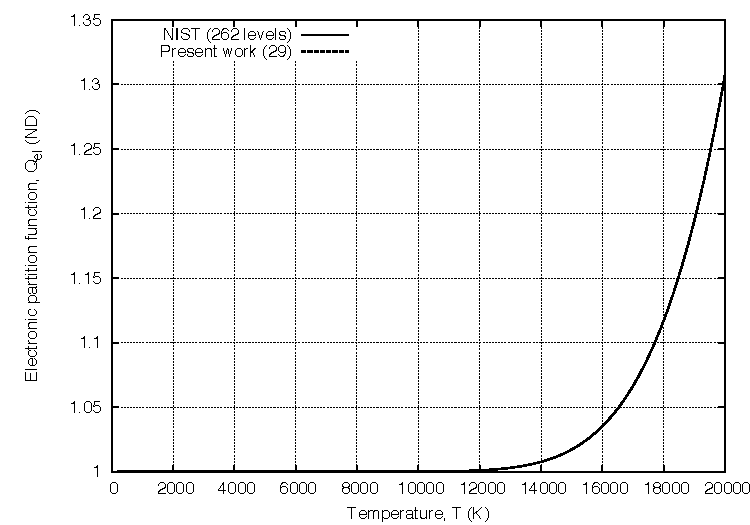
\includegraphics[width=0.5\linewidth]{figures/spectral-modelling/Ar_QvT.pdf} \label{fig:Ar_QvT}} 
 \subfloat[Atomic argon cation, Ar$^+$]{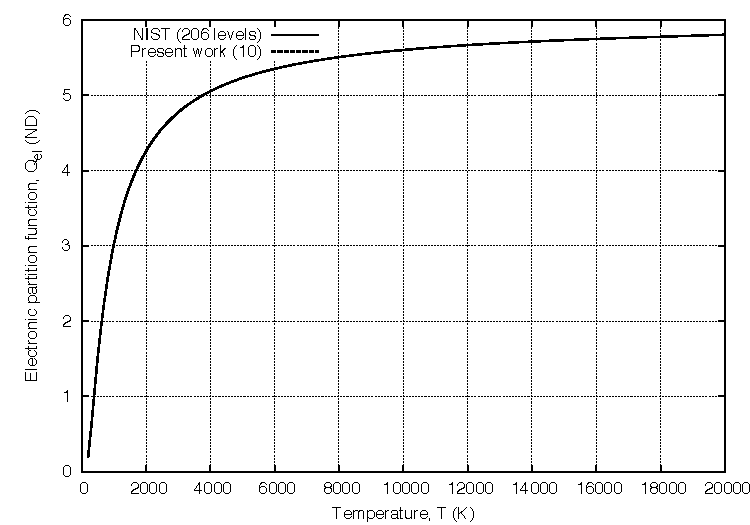
\includegraphics[width=0.5\linewidth]{figures/spectral-modelling/Ar_plus_QvT.pdf} \label{fig:Ar_plus_QvT}} \\
 \subfloat[Atomic carbon, C]{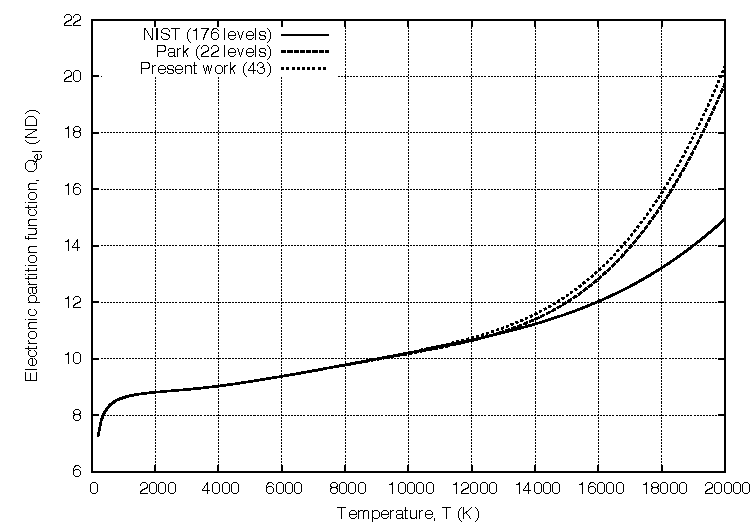
\includegraphics[width=0.5\linewidth]{figures/spectral-modelling/C_QvT.pdf} \label{fig:C_QvT}} 
 \subfloat[Atomic carbon cation, C$^+$]{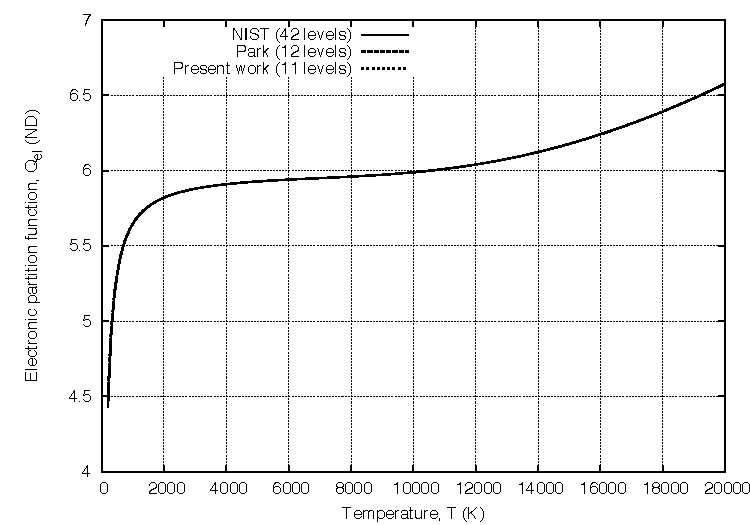
\includegraphics[width=0.5\linewidth]{figures/spectral-modelling/C_plus_QvT.pdf} \label{fig:C_plus_QvT}} \\
 \subfloat[Atomic nitrogen, N]{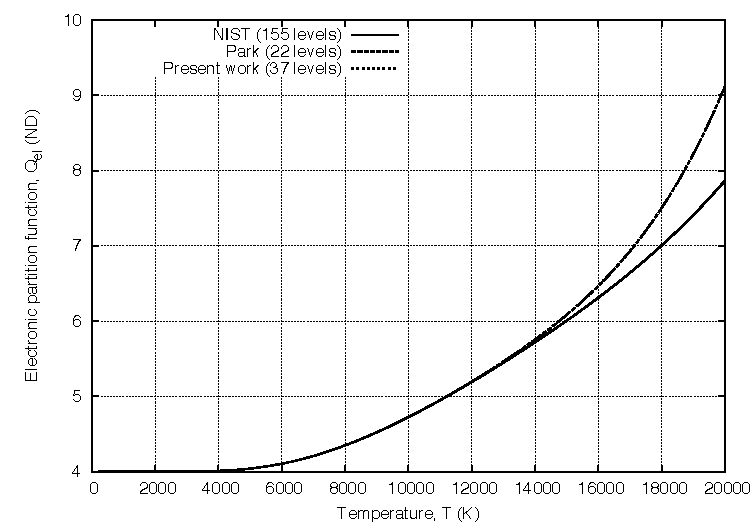
\includegraphics[width=0.5\linewidth]{figures/spectral-modelling/N_QvT.pdf} \label{fig:N_QvT}} 
 \subfloat[Atomic nitrogen cation, N$^+$]{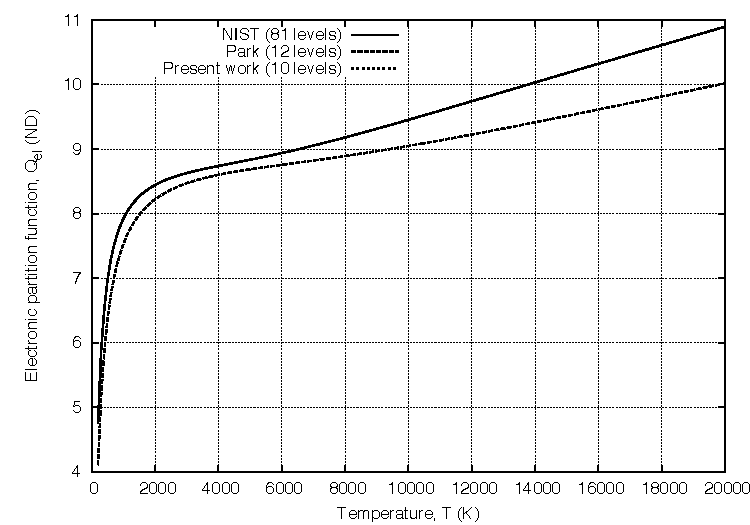
\includegraphics[width=0.5\linewidth]{figures/spectral-modelling/N_plus_QvT.pdf} \label{fig:N_plus_QvT}}
 \caption{Comparison of electronic partition function $Q_\text{el}$ for the monatomic radiators using various levels sets.}
 \label{fig:monatomic_QvT}
\end{figure}
%
\begin{figure}[!t]
 \centering
 \ContinuedFloat
 \subfloat[Atomic oxygen, O]{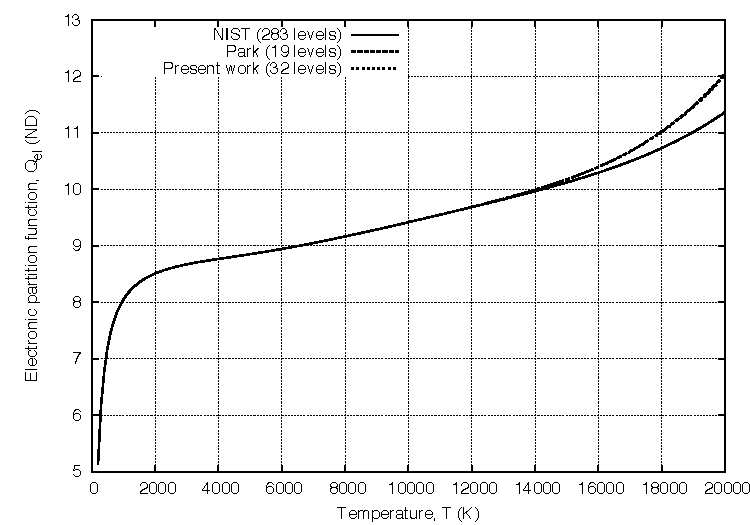
\includegraphics[width=0.5\linewidth]{figures/spectral-modelling/O_QvT.pdf} \label{fig:O_QvT}} 
 \subfloat[Atomic oxygen cation, O$^+$]{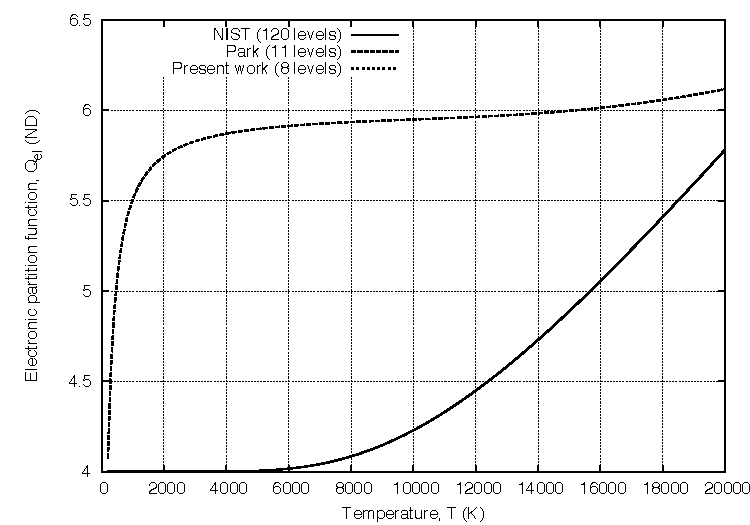
\includegraphics[width=0.5\linewidth]{figures/spectral-modelling/O_plus_QvT.pdf} \label{fig:O_plus_QvT}}
 \caption{\textit{(Continued)} Comparison of electronic partition function $Q_\text{el}$ for the monatomic radiators using various levels sets.}
 \label{fig:monatomic_QvT}
\end{figure}

\subsubsection{Electronic transitions}

Table~\ref{tab:atomic-lines} summarises the lines considered for monatomic species in the present work.
Following the recommendations of Johnston~\cite{JohnPhd}, when performing radiatively coupled Navier--Stokes simulations transitions with energy less than 6~eV are modelled as multiplet lines whilst higher energy transitions are modelled as individual lines.
This line selection strategy was shown in Reference~\cite{JohnPhd} to enable the radiant energy to be accurately captured whilst optimising the efficiency of the calculation.
It should be noted that the multiplet treatment of spectral lines inevitably leads to some error in the transport calculation, and future work should seek to treat all lines individually if sufficient computational resources are available to make the calculations possible.
Also, when performing comparisons with experimental spectra in the present work, all lines are treated individually to best represent the observed spectra.
This is possible as the single line-of-sight calculations required for spectra comparisons are not computationally intensive.

\begin{table}[h]
 \center
 \caption{Summary of atomic electronic levels and lines from the NIST Atomic Spectra Database~\cite{NIST_ASD} implemented in the present work.}
 \label{tab:atomic-lines}
 \begin{tabular*}{0.8\textwidth}{cccccc}
  \hline Species                          & \multicolumn{2}{c}{Number of individual lines}                                  & \multicolumn{2}{c}{Number of multiplet lines}      \\
                                                      &$\Delta E \leq 6$\,eV & $\Delta E > 6$\,eV                                           & $\Delta E \leq 6$\,eV & $\Delta E > 6$\,eV \\
  \hline  
                  Ar                               &  422                             &  6                                      &   204                            &    6                          \\
                  Ar$^+$                      &   297                            & 10                                    &   98                               &    3                         \\
                  C                                & 1141                            & 157                                 &  390                              &    56                       \\
                  C$^+$                       &   358                             & 278                                 &  89                                 &    69                       \\
                  N                                &    970                            & 129                                 & 223                                &    44                       \\      
                  N$^+$                       &    481                            & 241                                 & 71                                   & 89                        \\
                  O                               &     691                            & 163                                 & 125                                &  55                        \\
                  O$^+$                      &    617                             &  259                               & 175                                 & 77                         \\            
  \hline
 \end{tabular*}
\end{table}

\par

As the electronic level data for each atomic species used for partition function calculations consists of multiplet and grouped levels, a mapping strategy is required for calculating the upper and lower line state populations.
This is achieved by assuming Boltzmann equilibrium with the associated multiplet or grouped electronic level.
For an upper state of a line denoted by $\ast$ with associated grouped electronic level $i$, for example, the upper state population is calculated as:

\begin{equation}
 N^\ast = N_i \frac{g^\ast}{g_i} \text{~exp} \left [ \frac{- ( E^\ast - E_i ) }{kT_\text{el}} \right ]
\end{equation}

\noindent where the associated grouped electronic levels for each line are determined from the NIST tabulations upon initialisation.

\subsubsection{Spectral distribution function}

The spectral distribution function $b(\nu)$ in Equations~\ref{eq:atomic_j_nu_ul} and~\ref{eq:atomic_kappa_nu_lu} describes the spectral distribution of the emission and absorption coefficients of a line transition. 
Although the energy gap characterising a transition is discrete, the energy spectrum of the resulting photon is smeared over a finite range due to various broadening mechanisms.
These broadening mechanisms can be classified into two types: those described by a Lorentzian distribution, and those described by a Gaussian distribution. 
The Lorentzian broadening mechanisms considered in the present work for monatomic radiators are:

\begin{itemize}
 \item Resonant pressure broadening
 \item Van der Waals broadening
 \item Stark broadening
 \item Natural broadening
\end{itemize}

\noindent The only Gaussian broadening mechanism considered is Doppler broadening.
The resultant spectral distribution function is therefore modelled as a Voigt profile which is a convolution of a Lorentzian and a Gaussian distribution.
A Gaussian and Lorentzian profile with equal half-widths and the convolved Voigt profile are shown in Figure~\ref{fig:voigt-profile}.
The Gaussian profile exhibits a rapid rise to the central peak, whilst the Lorentzian profile is characterised by slowly decaying `wings'.

\par

\begin{figure}[h]
 \centering
 \subfloat[Linear $b(\nu)$ representation]{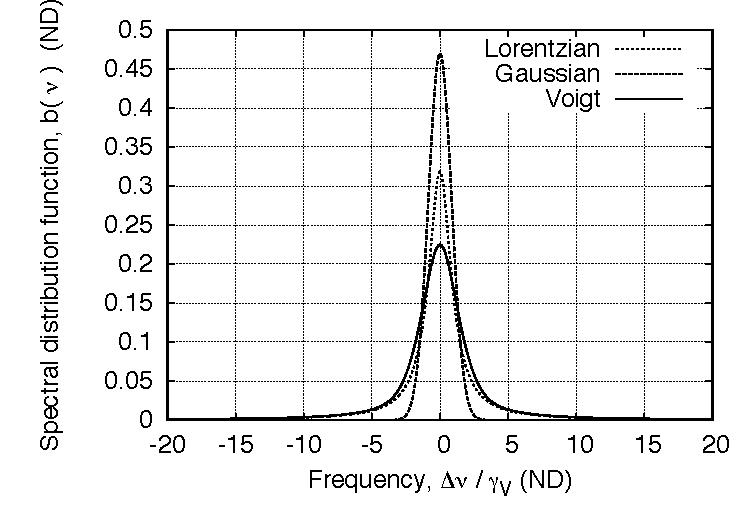
\includegraphics[width=0.5\linewidth]{figures/spectral-modelling/voigt-profile-linear.pdf}}
 \subfloat[Logarithmic $b(\nu)$ representation]{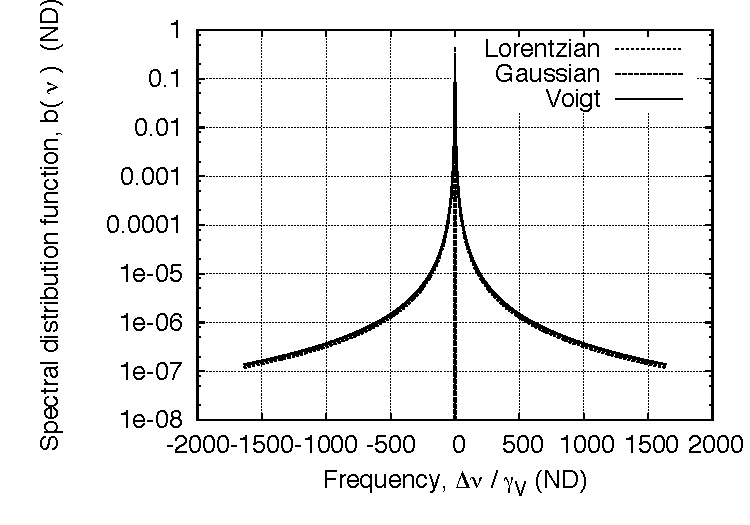
\includegraphics[width=0.5\linewidth]{figures/spectral-modelling/voigt-profile-log.pdf}}
 \caption{Gaussian, Lorentzian and Voigt profiles as a function of the normalised frequency.  The Gaussian and Lorentzian profiles have the same half-widths.}
 \label{fig:voigt-profile}
\end{figure}

In the present work the Voigt profile approximation proposed by Whiting~\cite{Whi68} is implemented:

\begin{equation}
 b(\nu) = \frac{\left ( 1 - R_D \right ) \text{~exp} \left ( -2.772 R_L^2 \right ) + \frac{R_D}{1 + 4 R_L^2} + 0.016 ( 1- R_D ) R_D \text{~exp} \left ( \frac{-0.4 R_L^{2.25} - 10}{10 + R_L^{2.25}} \right )}{2 \gamma_V \left ( 1.065 + 0.447 R_D + 0.058 R_D^2 \right )}
\end{equation}

\noindent where $R_D$ and $R_L$ are defined as:

\begin{eqnarray}
 R_D = \frac{\gamma_L}{\gamma_V} \text{ , and }
 R_L  = \frac{\nu_{ul}}{2 \gamma_V} \text{ , }
\end{eqnarray}

\noindent and $\gamma_L$, $\gamma_D$ and $\gamma_V$ are respectively the Lorentzian, Doppler and Voigt half-widths at half-maximum (HWHM) in frequency units.
The Voigt half-width is a function of the Lorentzian and Doppler (Gaussian) half-widths, and is calculated by the following approximation of Olivero and Longbothum~\cite{olivero}:

\begin{equation}
 \gamma_V = \left ( 1 - 0.18121 ( 1 - d^2 ) - \left [ 0.023665 \text{~exp} \left ( 0.6 d \right )  + 0.0418 \text{~exp} \left ( -1.9 d \right ) \text{sin}(\pi d) \right ] \right ) \left ( \gamma_L + \gamma_D \right )
\end{equation}

\noindent where $d$ is defined as:

\begin{equation}
 d = \frac{ \gamma_L - \gamma_D }{ \gamma_L + \gamma_D } \text{ . }
\end{equation}

The Lorentzian half-width $\gamma_L$ is the sum of the contributions from the Lorentzian broadening mechanisms:

\begin{equation}
 \gamma_L = \gamma_R + \gamma_{VW} + \gamma_S + \gamma_N
\end{equation}

\noindent where $ \gamma_R$, $ \gamma_VW$, $\gamma_S$ and $\gamma_N$ are the resonance, Van der Waals, Stark and natural broadening half-widths respectively.
Resonant pressure broadening is modelled via the expression of Nicolet~\cite{Nic70}:

\begin{equation}
 \gamma_R = 3 \pi \sqrt{\frac{g_l}{g_u}} \left [ \frac{e^2 f_{lu}}{2 \pi m \nu_{ul}} \right ] N_a
\end{equation}

\noindent where $f_{lu}$ is the transition oscillator strength and $N_a$ is the number density of perturbing atoms.
In the present work $N_a$ is set to the number density of the lower state.
Van der Waals broadening accounts for pressure broadening due to non-resonant interactions, and is modelled by the expression given by Traving~\cite{Traving95}:

% check this expression in the reference
\begin{equation}
 \gamma_{VW} = 1.95 \times 10^{-28} \sqrt{ \frac{2 T}{M_\text{av}} } N_\text{hp} \nu_{ul}^2
\end{equation}

\noindent where $M_\text{av}$ is the average molecular weight of the mixture and $N_\text{hp}$ is the heavy particle number density.
Although accurate Stark widths for some atomic species are tabulated in the literature (\textit{e.g.} Reference~\cite{Griem64}), in the present work Stark broadening is modelled via the following approximate expression observed by Page~\cite{PCB+1968}:

\begin{equation}
 \gamma_S =  \gamma_{S}^{0} \left ( \frac{T_e}{T_e^0} \right )^{\alpha_S} \left ( \frac{N_e}{N_e^0} \right )
 \label{eq:stark}
\end{equation}

\noindent where $\alpha_S$ is a fitting constant and $\gamma_{S}^{0}$ is a reference Stark half-width per electron at electron temperature $T_e^0$ and electron number density $N_e^0$.
The reference half-widths are approximated by the following curve-fit proposed by Johnston ~\cite{JohnPhd}\footnote{Note that the original expression presented by Johnston~\cite{JohnPhd} is for the full-width in wavelength units, whereas that presented here is for the half-width in frequency units.}:

\begin{equation}
 \gamma_S^0 = \frac{8.45 \times 10^{9}}{ \left ( I - E_u \right )^{2.623}}
\end{equation}

\noindent where the reference electron temperature $T_e^0$ and number density $N_e^0$ are 10,000\,K and $1 \times 10^{16}$\,cm$^{-1}$ respectively, and the fitting constant $\alpha_S$ is set to 0.33.
 This curve-fit is shown in Reference~\cite{JohnPhd} to be a good approximation of the accurate N and O Stark widths presented by Griem~\cite{Griem64} and others.
Natural line broadening is modelled using the following classical expression~\cite{Thorne74}:

\begin{equation}
 \gamma_N = \frac{2 \pi e^2 \nu_{ul}^2 }{3 \epsilon_0 m c^3}
\end{equation}

\noindent and Doppler broadening is modelled by the half-width expression given by Nicolet~\cite{Nic70}:

\begin{equation}
 \gamma_D = \frac{\nu_{ul}}{c} \sqrt{ \frac{2 k_B T_\text{tr} \text{ln}(2)}{m_s} }
\end{equation}

\noindent where $m_s$ is the species mass per particle.

\par

Figures~\ref{fig:air-BL-linewidths} and~\ref{fig:air-SL-linewidths} compare the monatomic half-widths calculated at conditions characteristic of typical lunar return peak heating gas states in the boundary and shock layers respectively (Fire II $t=1642.66$\,s).
The line widths in the boundary layer are dominated by Doppler broadening with Van der Waals broadening becoming significant at the higher wavelengths, whilst those in the shock layer are largely dominated by Stark broadening.
Furthermore the Stark widths in the shock layer are on average approximately $10^3$ times greater than in the boundary layer.
This is explained by the much higher free electron temperature and density in the shock layer, and that the Stark width is proportional to $T_e^{1/3} N_e$.
In both the boundary and shock layers the natural and resonance broadening contributions are negligible for the spectral range considered.
%Note that the lower $\gamma$ range in Figure~\ref{fig:air-BL-linewidths} has been set to $1 \times 10^{-25}$\,$\AA$ for clarity, although the average resonance half-width between 200 and 2,000\,nm is approximately $1 \times 10^{-40}$\,$\AA$.

\begin{figure}[p!]
 \center
 \subfloat[Boundary layer conditions ($T_\text{tr}=3,510$\,K, $T_\text{ve}=3,870$\,K, $p=77,900$\,Pa and $N_e=1.8 \times 10^{13}$\,cm$^{-1}$)]{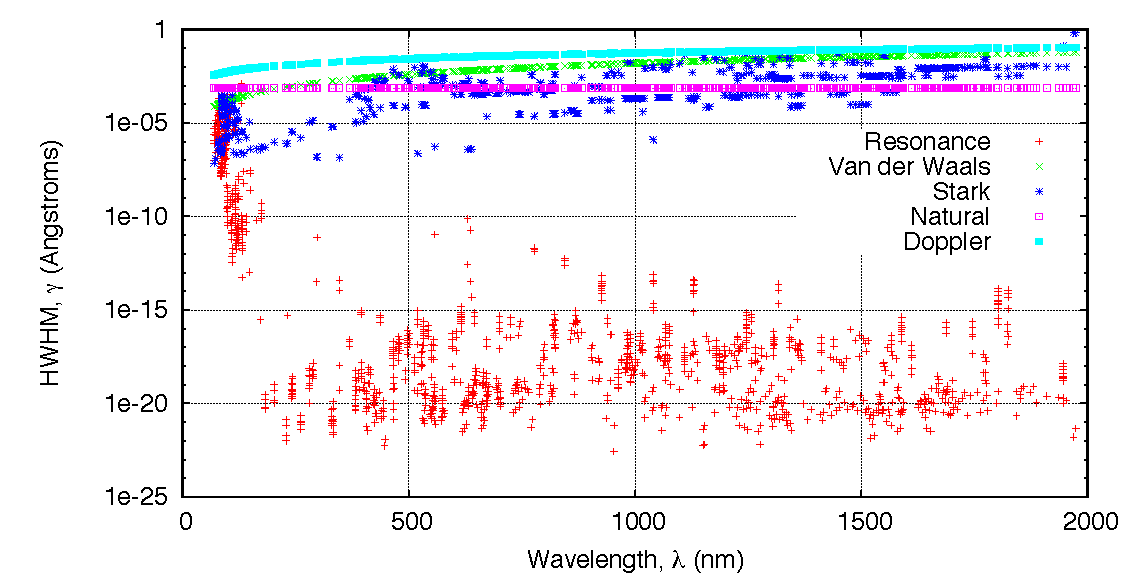
\includegraphics[width=\linewidth]{figures/spectral-modelling/air_BL_linewidths.pdf} \label{fig:air-BL-linewidths}} \\
 \subfloat[Shock layer conditions ($T_\text{tr}=11,220$\,K, $T_\text{ve}=11,200$\,K, $p=79,000$\,Pa and $N_e=3.6 \times 10^{16}$\,cm$^{-1}$)]{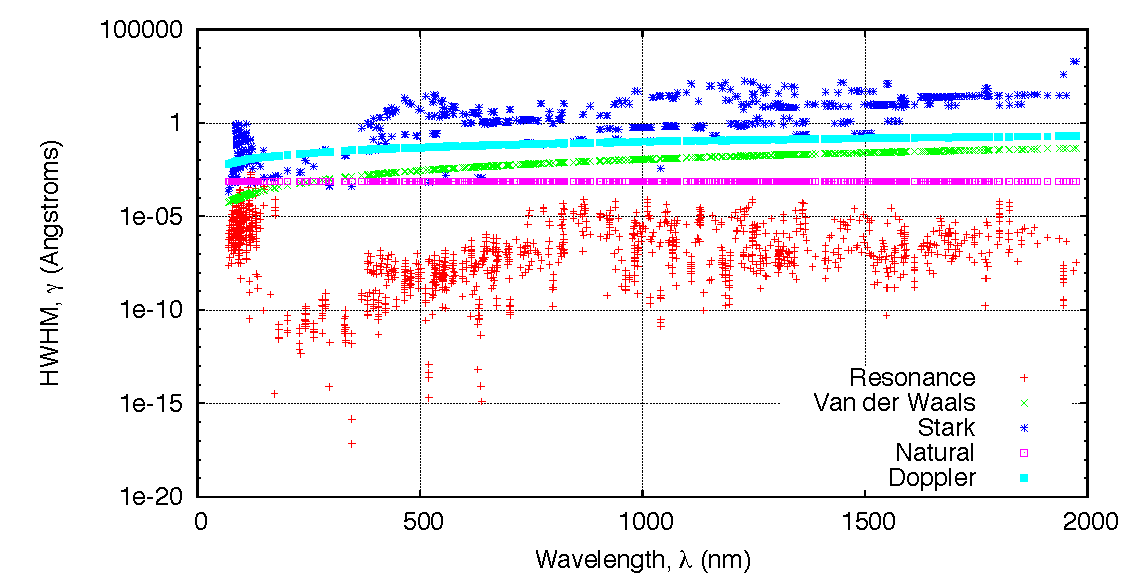
\includegraphics[width=\linewidth]{figures/spectral-modelling/air_SL_linewidths.pdf} \label{fig:air-SL-linewidths}}
 \caption{Monatomic line half-widths at half-maximum for typical Lunar return peak heating conditions (Fire II $t=1642.66$\,s).}
 \label{fig:air-linewidths}
\end{figure}

 \begin{figure}[p!]
 \center
 \subfloat[Boundary layer conditions ($T_\text{tr}=2,970$\,K, $T_\text{ve}=2,550$\,K, $p=29,500$\,Pa and $N_e=2.3 \times 10^{13}$\,cm$^{-1}$)]{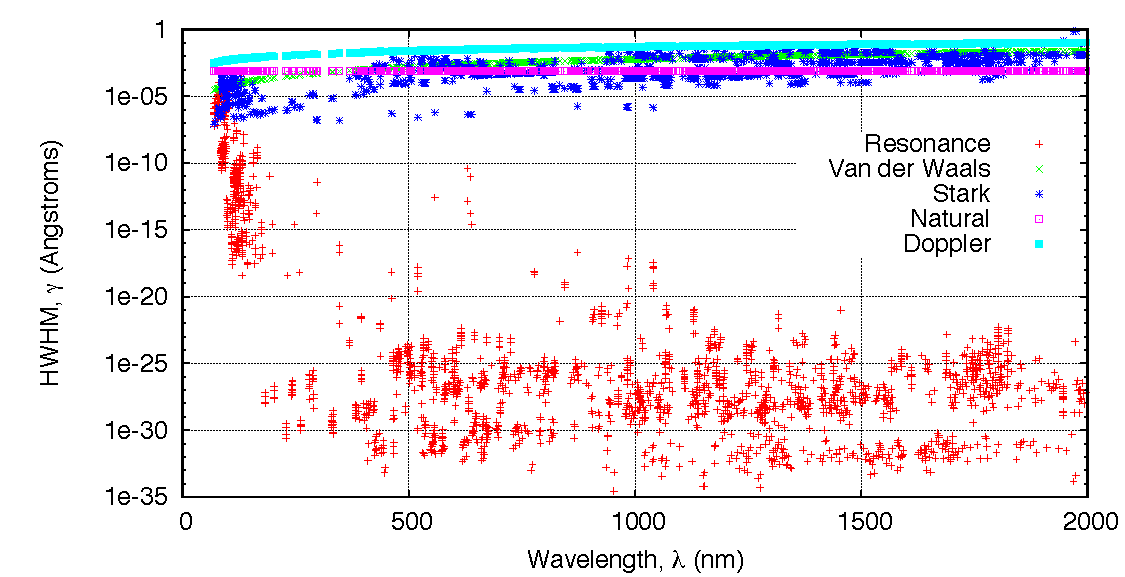
\includegraphics[width=\linewidth]{figures/spectral-modelling/mars_BL_linewidths.pdf} \label{fig:mars-BL-linewidths}} \\
 \subfloat[Shock layer conditions ($T_\text{tr}=6,930$\,K, $T_\text{ve}=6,930$\,K, $p=29,500$\,Pa and $N_e=7.7 \times 10^{14}$\,cm$^{-1}$)]{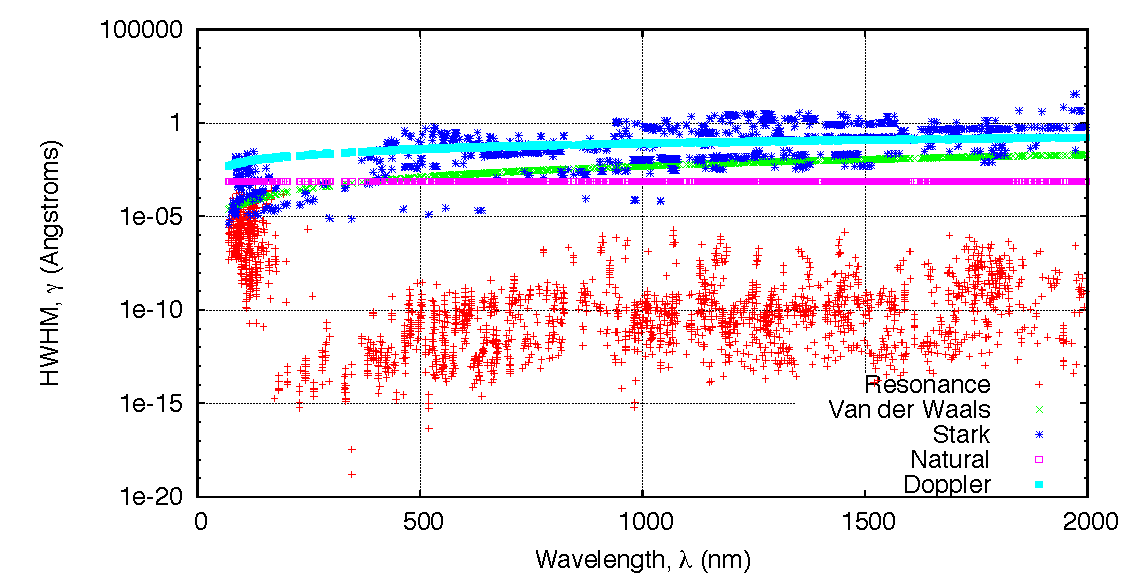
\includegraphics[width=\linewidth]{figures/spectral-modelling/mars_SL_linewidths.pdf} \label{fig:mars-SL-linewidths}}
 \caption{Monatomic line half-widths at half-maximum for a hypothetical high-speed Mars entry trajectory point with a freestream pressure and velocity of 18\,Pa and 8\,km/s respectively.}
 \label{fig:mars-linewidths}
\end{figure}

\par 

Figures~\ref{fig:mars-BL-linewidths} and~\ref{fig:mars-SL-linewidths} compare the monatomic half-widths calculated at conditions characteristic of a hypothetical high-speed Mars entry trajectory point with a freestream pressure and velocity of 18\,Pa and 8\,km/s respectively.
Here the line widths in the boundary layer are also dominated by Doppler broadening, with both Stark and Van der Waals broadening making minor contributions especially at the higher wavelengths.
In contrast to the lunar return case, both Stark and Doppler broadening make approximately equal contributions to the line widths for the Mars entry shock layer.
This is due to the signicantly lower free electron number density and temperature for the Mars entry case.
From these results it is evident that both natural and resonance broadening can be omitted without significant loss of line width accuracy for the thermodynamic regimes of present interest.


\par

% sensitivity of I_total for 50 < lambda < 200nm to:
% - line extent

Finally, an appropriate cut-off limit for each line must be determined.
Although the wings of the Voigt profile are many orders of magnitude weaker than the central peak (see Figure~\ref{fig:voigt-profile}), the wings extend far beyond the line-centre and the rate of decay is low.
Figures~\ref{fig:atomic-EvLE} and~\ref{fig:atomic-IvLE} compare the sensitivity of atomic bound-bound emissive power density and intensity for a 10\,cm slab of atmospheric pressure equilibrium air to the atomic line cut-off limit.
The line cut-off limit $\Delta \nu_\text{limit}$ has been normalised by the voigt HWHM $\gamma_V$, and the emissive power density and intensity are normalised by the respective values at $\Delta \nu_\text{limit} = 10,000 \gamma_V$.
While the emissive power density is reasonably well described with $\Delta \nu_\text{limit} / \gamma_V \geq 10$, the intensity is much more sensitive, requiring $\Delta \nu_\text{limit} / \gamma_V \geq 1000$.
To optimise the efficiency of the calculation, it is desirable to use the minimum cut-off limit; therefore in the present work the atomic line cut-off limit is set to $\Delta \nu_\text{limit} = 1000 \gamma_V$.

\begin{figure}[h]
 \centering
 \subfloat[Emissive power density]{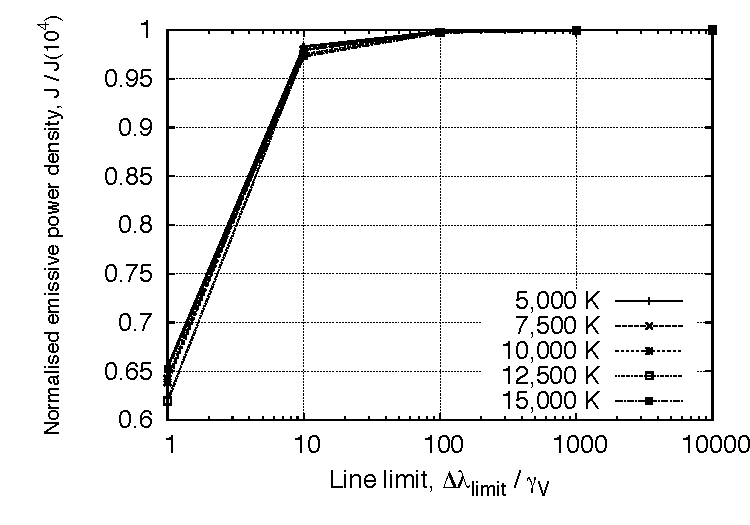
\includegraphics[width=0.5\linewidth]{figures/spectral-modelling/atomic-EvLineExtent.pdf} \label{fig:atomic-EvLE}}
 \subfloat[Intensity]{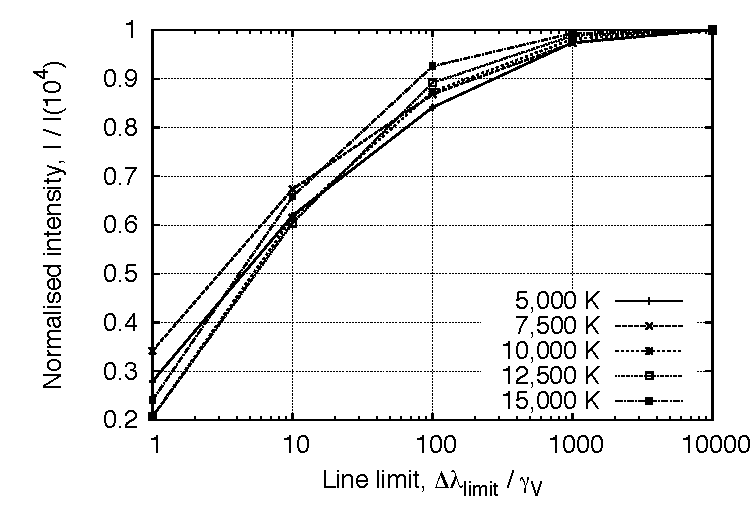
\includegraphics[width=0.5\linewidth]{figures/spectral-modelling/atomic-IvLineExtent.pdf} \label{fig:atomic-IvLE}}
 \caption{Sensitivity of atomic bound-bound emissive power density and intensity for a 10\,cm slab of equilibrium air to the atomic line cut-off limit ($p=1$\,atm).}
 \label{fig:atomic_LE_sensitivity}
\end{figure}


\subsubsection{Comparison with SPRADIAN07}

The Structured Package for Radiation Analysis 2007 (SPRADIAN07) program has been recently developed by the Japanese Aerospace Exploration Agency (JAXA) and Korea Advanced Institute of Science and Technology (KAIST).
The theory and implementation of SPRADIAN07 is described in the PhD thesis of Hyun~\cite{hyun_phd}.
Both SPRADIAN07 and the model developed in the present work implement the spectroscopic data from the NIST Atomic Spectra Database~\cite{NIST_ASD}.
Comparisons with the SPRADIAN07 code~\cite{hyun_phd} have therefore been made in order to verify the calculation of atomic bound-bound spectral coefficients.
The test case consists of a 10\,cm slab of gas with temperature $T=10,000$\,K and pressure $p=1$\,atm.
The number density of each radiator is $1 \times 10^{16}$\,cm$^{-3}$, the electron number density is also $1 \times 10^{16}$\,cm$^{-3}$ and total number density is $2.2 \times 10^{17}$\,cm$^{-3}$.
The bound-bound transitions of Ar, Ar$^+$, C$^+$, N$^+$, O$^+$ are not included in the comparison as the SPRADIAN07 code does not consider them.
For each radiator, the emissive power density $J$ (W/cm$^3$) and intensity $I$ (W/cm$^2$) is calculated in the spectral range $ 50 \leq \lambda \leq 2,000$\,nm with 1,950,000 equidistant frequency intervals.  

\par

Table~\ref{tab:spradian_atom_compare} summarises the comparison between the SPRADIAN07 code~\cite{hyun_phd} and the present work for atomic bound-bound transitions.
While the agreement for emissive power density is within 1\% for all the key atomic radiators, the SPRADIAN07 predicts between 16 and 28\% lower intensity through the 10\,cm slab.
The difference in intensity can be attributed to slight discrepancies in the line half-widths.
Figures~\ref{fig:0-133nm-line-emission},~\ref{fig:0-133nm-line-abs} and~\ref{fig:0-133nm-line-intensity} presents the intensity, absorption coefficient and emission coefficient spectra for the atomic oxygen lines in the spectral range $128 \leq \lambda \leq 133$\,nm.
The SPRADIAN07 emission and absorption spectra peaks higher and drops lower than that from the present work, indicating the SPRADIAN07 line-widths for these transitions are slightly lower.
The resultant cumulative intensity is almost 25\% lower, however, indicating the high sensitivity of intensity to the line half-widths.
While the SPRADIAN07 code uses experimentally determined Stark broadening parameters, the present model uses an approximate curve-fit.
Unfortunately the approximate method for calculating the Stark width is a limitation of the spectral model developed for the present work.

\begin{table}[h]
 \small
 \center
 \caption{Comparison of atomic bound-bound model from the present work with the SPRADIAN07 code~\cite{hyun_phd}.}
 \label{tab:spradian_atom_compare}
 \begin{tabular*}{1.0\textwidth}{ccccccc}
  \hline Species                          & \multicolumn{3}{c}{Emissive power density, $J$ (W/cm$^3$)}        & \multicolumn{3}{c}{Intensity, $I$ (W/cm$^2$)}      \\
                                                      & SPRADIAN07 & Present work & Difference (\%)                      & SPRADIAN07 & Present work & Difference (\%) \\
  \hline  
                  C                                & 1265              & 1269      & 0.34                                                  & 20.58            & 25.76  &  20.12 \\
                  N                                &  179.8            &  181.0    & 0.65                                                  & 3.77              & 4.54     &  16.92 \\
                  O                                &  59.85            &    60.28  & 0.72                                                  & 1.55              & 2.13     &  27.35 \\
  \hline
 \end{tabular*}
\end{table}

\begin{figure}[p]
 \centering
 \subfloat[Emission]{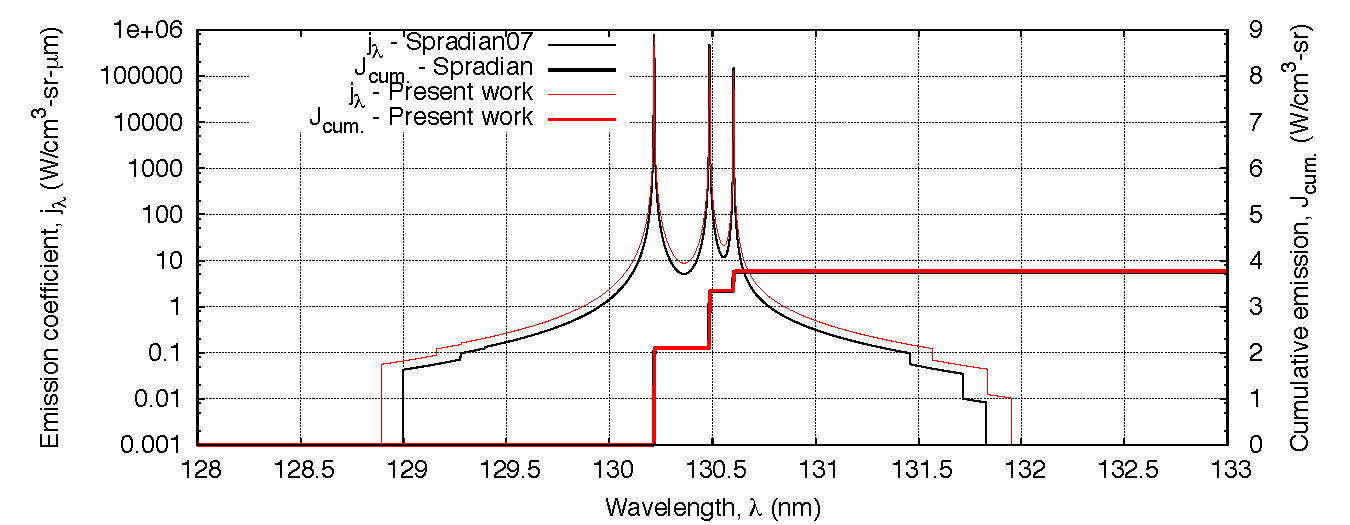
\includegraphics[width=1.0\linewidth]{figures/spectral-modelling/O-133nm-line-emission.pdf}  \label{fig:0-133nm-line-emission}} \\
 \subfloat[Absorption]{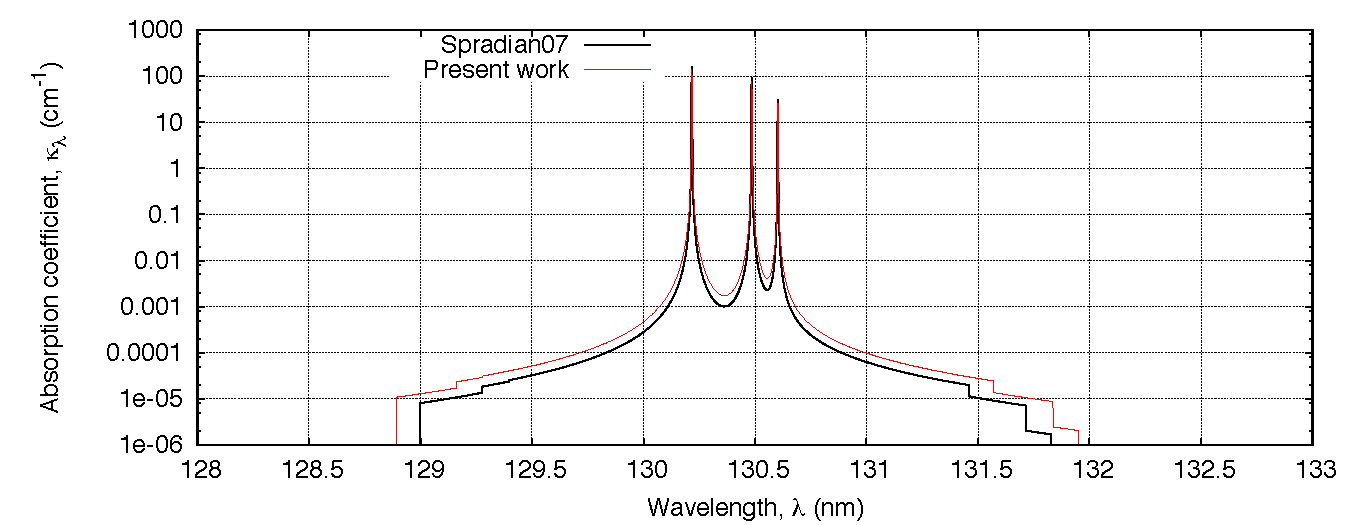
\includegraphics[width=1.0\linewidth]{figures/spectral-modelling/O-133nm-line-abs.pdf}  \label{fig:0-133nm-line-abs}} \\
 \subfloat[Spectral and cumulative intensity]{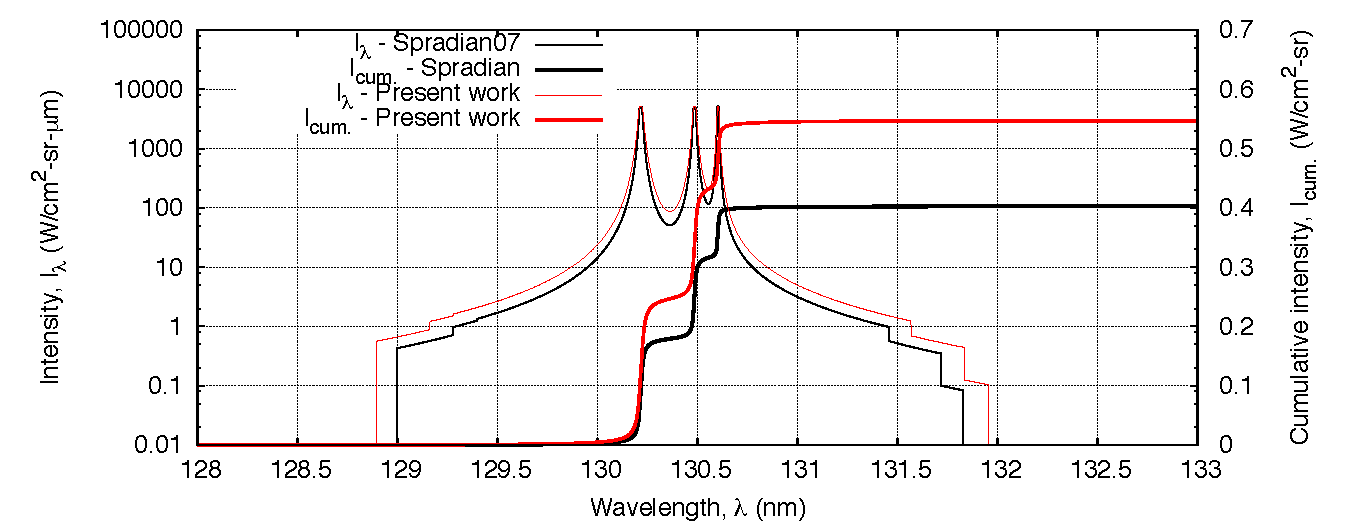
\includegraphics[width=1.0\linewidth]{figures/spectral-modelling/O-133nm-line-intensity.pdf}  \label{fig:0-133nm-line-intensity}}
 \caption{Comparison between SPRADIAN07 and the present work for the spectra of atomic oxygen lines in the range $128 \leq \lambda \leq 133$\,nm.}
\end{figure}


\subsection{Diatomic bound-bound transitions}
\label{sec:diatomic_transitions}

Diatomic bound-bound transitions occur between individual rovibronic\footnote{A rovibronic state is a molecular configuration with a complete set of rotational, vibrational and electronic quantum numbers.} states of the molecule.
The resulting rotational lines are clustered into bands and systems corresponding to individual vibrational and electronic transition groups.
The spectral emission and absorption coefficients for an individual diatomic bound-bound transition are the same as for monatomic transitions:

\begin{equation}
 j_{\nu,ul} = \frac{n_{u} h \nu_{u l} A_{u l}}{4 \pi} b_{ul}(\nu) \label{eq:diatomic_j_nu_ul}
\end{equation}

\begin{equation}
 \kappa_{\nu,lu} = \left ( n_l \frac{g_u}{g_l} - n_u \right ) \frac{c^2}{8 \pi \nu_{ul}^2} A_{ul} b_{ul}(\nu) \label{eq:diatomic_kappa_nu_lu}
\end{equation}

\noindent where $l$ and $u$ denote the lower and upper energy levels, $n$ is the level number density, $A_{ul}$ is the Einstein coefficient for spontaneous emission and $b_{ul}(\nu)$ is the spectral distribution function.

% explain the coupling cases considered here

\subsubsection{Rovibronic transitions}

The determination of allowed transitions, their energies and probabilities is dependent on the coupling between electronic orbital $\vec{L}$, electron spin $\vec{S}$ and nuclear rotation $\vec{N}$ angular momentum vectors for the upper and lower rovibronic states.
The Hund's coupling cases\footnote{A fifth coupling case (e) theoretically exists where $\vec{L}$ and $\vec{S}$ are strongly coupled, however such behaviour has not been observed for any species~\cite{HH_1979}.} (a), (b), (c) and (d) illustrated in Figure~\ref{fig:hunds_cases} define idealised limiting cases of angular momentum couplings~\cite{HH_1979}. 
In Hund's case (a) nuclear rotation is completely decoupled from electronic motion, whilst electronic motion is strongly coupled to the internuclear axis.
In Hund's case (b) electron spin decouples from the internuclear axis due to strong coupling with the rotational motion.
When the interaction between the electronic orbital and electron spin angular-momentum is very strong we have Hund's case (c), and when the electronic orbital is strongly coupled to the axis of rotation we have Hund's case (d).

\begin{figure}[ht]
 \center
 \subfloat[Case (a)]{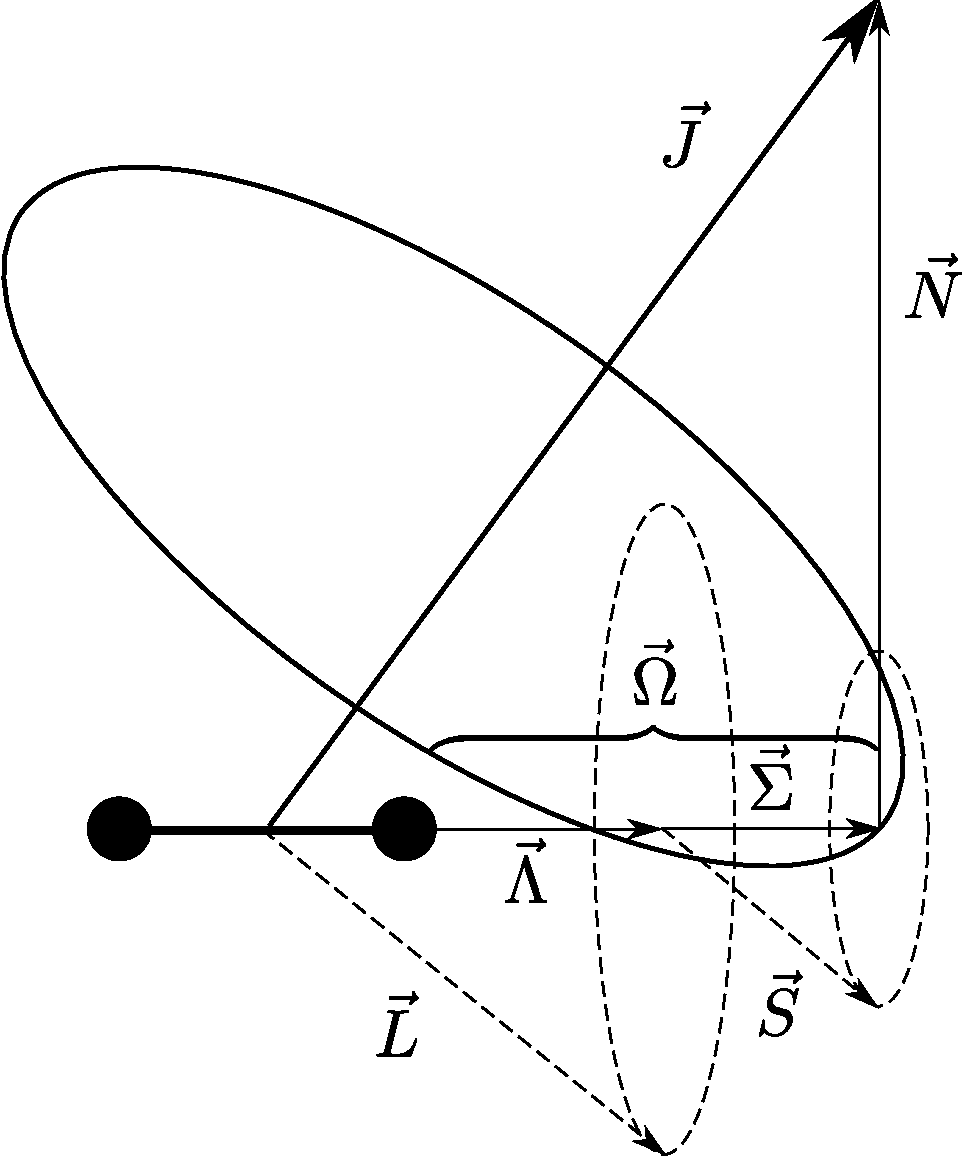
\includegraphics[width=0.2\linewidth]{figures/spectral-modelling/hunds_case_A.pdf}}
 \hspace{0.5cm}
 \subfloat[Case (b)]{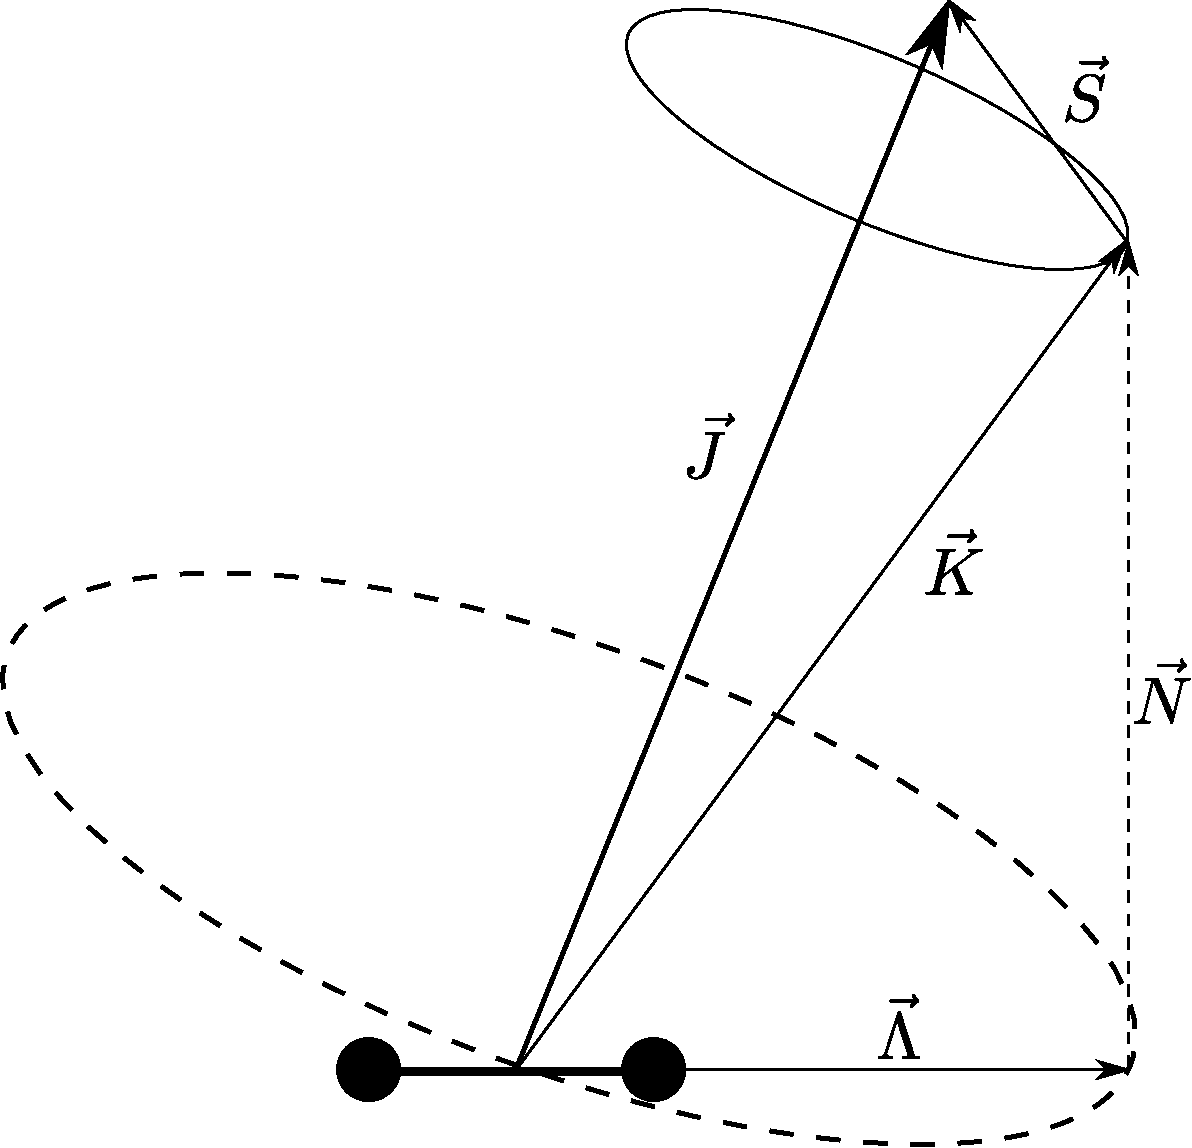
\includegraphics[width=0.2\linewidth]{figures/spectral-modelling/hunds_case_B.pdf}}
 \hspace{0.5cm}
  \subfloat[Case (c)]{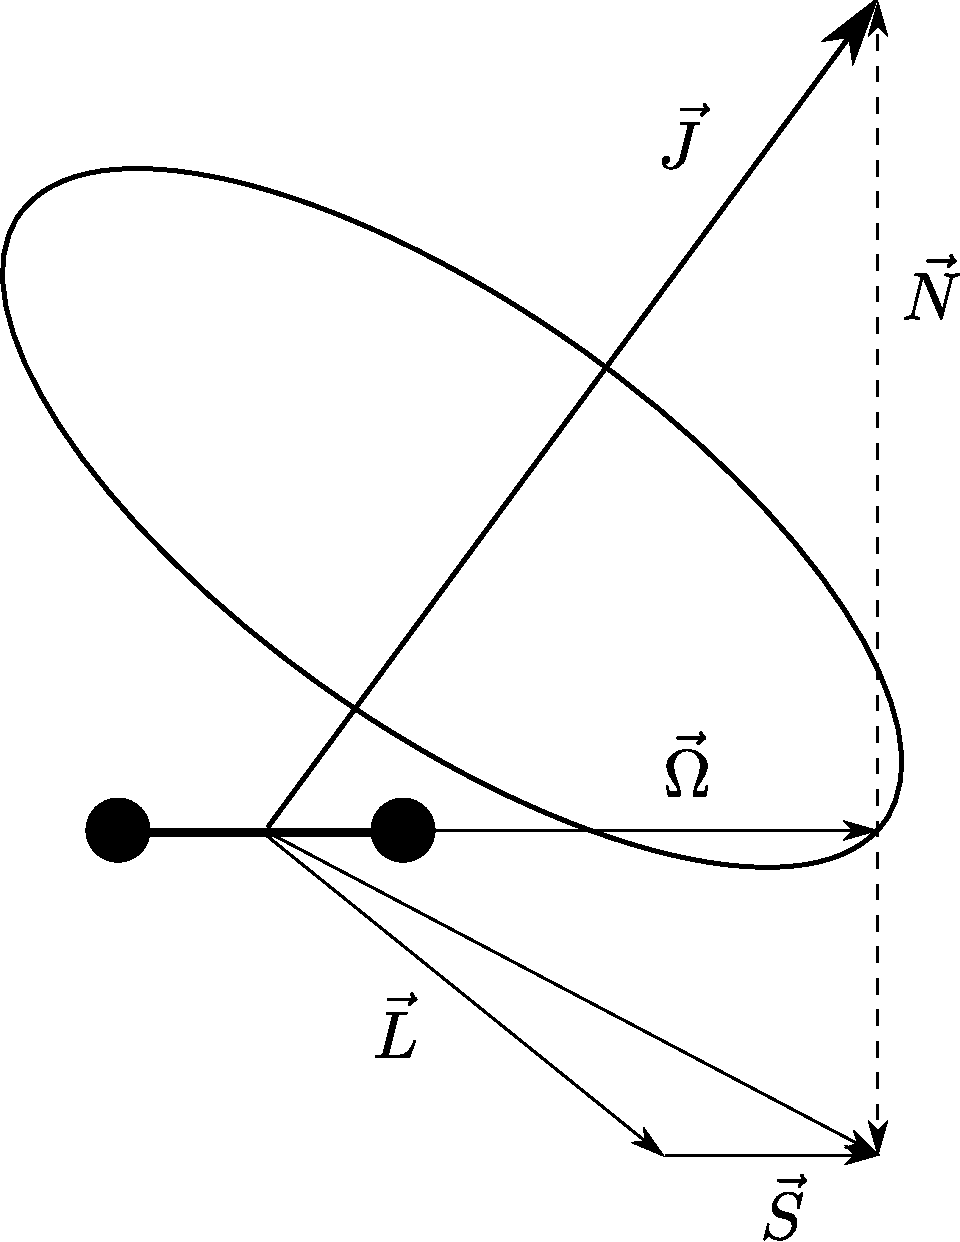
\includegraphics[width=0.2\linewidth]{figures/spectral-modelling/hunds_case_C.pdf}}
 \hspace{0.5cm}
 \subfloat[Case (d)]{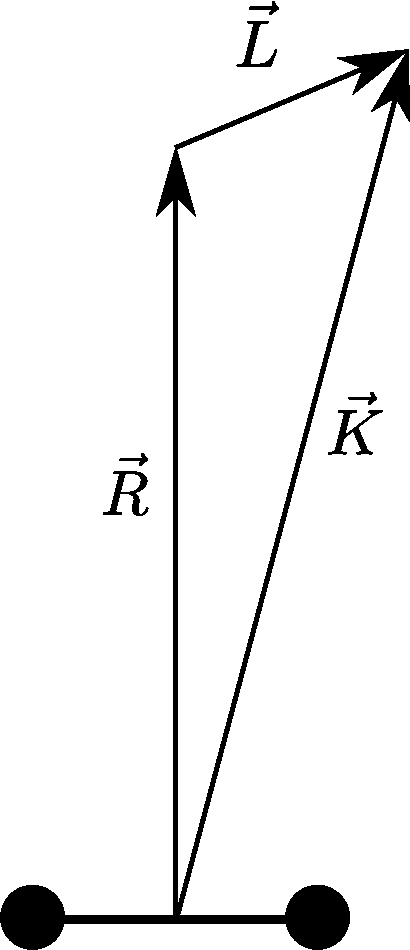
\includegraphics[width=0.08\linewidth]{figures/spectral-modelling/hunds_case_D.pdf}}
 \caption{Diagrammatic representations of the (a), (b), (c) and (d) Hund's coupling cases describing the limiting angular momentum interactions for rovibronic transitions.}
 \label{fig:hunds_cases}
\end{figure}

% state full equations for spectral emission and absorption coefficients here

\par

In the present work we consider cases (a) and (b) and an intermediate (a)-(b) case.
This selection is a good compromise between speed and accuracy, as spin splitting is captured when important whilst $\Lambda$-type doubling which involves much finer perturbations is neglected.
Here we will present a brief overview of the selection rules for these three transitions; for a complete discussion the reader is directed to the texts of Huber and Herzberg~\cite{HH_1979} and Kov\'{a}cs~\cite{kovacs69}.
The energy and transition probability expressions for each case will be presented in the following sections.

\par

For all coupling cases the selection rule for the total angular momentum quantum number $J$ is:

\begin{equation}
 J_u - J_l = \Delta J = 0,~\pm1 \text{, and } J_u = J_l \neq 0 \label{eq:delta_J_rules}
\end{equation}


For Hund's case (a) the electronic angular momentum $\vec{\Omega}$ and rotational angular momentum $\vec{N}$ couple to form the resultant angular momentum vector $\vec{J}$.
Therefore the total angular momentum quantum number $J$ cannot be smaller than the electronic component $\Omega = | \Lambda + \Sigma |$:

\begin{equation}
 J = \Omega,~\Omega + 1,~\Omega + 2,~\cdots
\end{equation}

An additional restriction for $\Sigma--\Sigma$ transitions belonging to Hund's case (a) is that $\Delta J=0$ transitions are universally prohibited.
Therefore Hund's case (a) transitions have three branches $P$, $Q$ and $R$ corresponding to $\Delta J = +1$, $0$ and $-1$ respectively, where only $P$ and $R$ branches exist for  $\Sigma--\Sigma$ transitions.
In the present work all singlet ($X^1 - X^1$ where $X = \Sigma, \Pi, \Delta,~\cdots$) and multiplet parallel ($X^n - Y^n$ where $n>1$ and $\left | L_m - L_n \right | =1$) transitions except from the CN Violet system are assumed to belong to Hund's case (a).

\par

For Hund's case (b) a total angular momentum quantum number \emph{apart from spin} $K$ is defined with one-to-one correspondence with $J$ as defined for Hund's case (a).
Therefore the selection rules pertaining to $J$ outlined above are now applied to $K$.
As $\vec{\Omega}$ and $\vec{N}$ are coupled in Hund's case (b), the permitted range for $K$ is:

\begin{equation}
 K = \Lambda,~\Lambda+1,~\Lambda+2,~\cdots
\end{equation}

As total angular momentum $\vec{J}$ is the resultant of $\vec{K}$ and the spin angular momentum $\vec{S}$, the possible values of $J$ are:

\begin{equation}
 J = ( K + S),~(K+S-1),~(K+S-2),~\cdots~, | K - S | .
\end{equation}

Therefore Hund's case (b) considers three $\Delta J$ branches that each consist of $2S+1$ spin split components.
In the present work only the CN Violet $\Sigma^2$ -- $\Sigma^2$ transition is described by Hund's case (b) coupling; for this transition, we have a total of 6 branches with designations $R_1$, $R_2$, $^{R}Q_{21}$, $^{P}Q_{12}$, $P_2$ and $P_1$.
Figure~\ref{fig:Violet_a_vs_b} compares the absorption coefficient for the CN Violet 0-0 band modelled via Hund's case (a) and Hund's case (b).
Although the two coupling cases produce similar results for branches close to the band head at 388.45~nm, the effect of spin splitting becomes more pronounced with increasing $J$.

\begin{figure}[htb]
 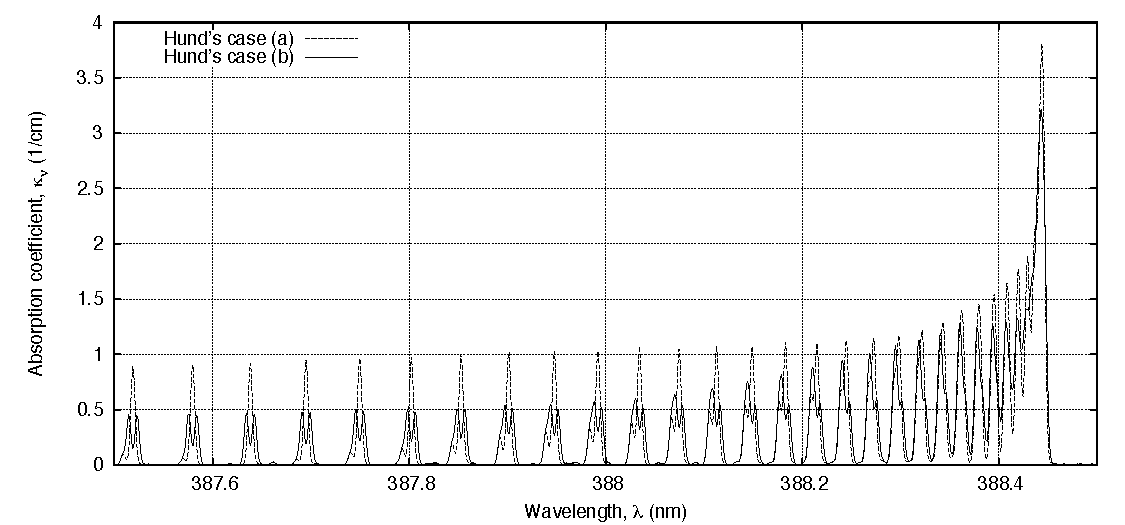
\includegraphics[width=\linewidth]{figures/spectral-modelling/CN_violet_absorption_coefficient_spectra_linear.pdf}
 \caption{Absorption coefficient for the CN Violet 0-0 band modelled via Hund's case (a) and Hund's case (b).}
 \label{fig:Violet_a_vs_b}
\end{figure}

\par

% currently just non-sigma doublets are described by case ab - the rest are hund's case a

The remaining transitions, which are the parallel doublets, are described by an intermediate (a)-(b) coupling case, where $\vec{S}$ is strongly coupled to the internuclear axis for low $J$ and becomes coupled with rotation with increasing $J$ -- hence this case is referred to as \textit{spin uncoupling}.
The quantum numbers $K$, $S$ and $J$ and their previous defined selection rules are all applicable to the intermediate (a)-(b) case.
Intermediate (a)-(b) coupling transitions have three $\Delta J$ branches each with $\left( 2S + 1 \right)^2$ spin split components.
A common transition that is modelled via the intermediate (a)-(b) coupling case is a perpendicular doublet such as $^2 \Pi$--$^2 \Sigma$.
These transitions have 12 branches with designations $P_{1}$, $P_2$, $P_{12}$, $P_{21}$, $Q_{1}$, $Q_2$, $Q_{12}$, $Q_{21}$, $R_{1}$, $R_2$, $R_{12}$ and $R_{21}$.

\subsubsection{Level populations}

% - state all partition functions
% - descend right down to rotational levels

The electronic level populations of molecular species are bounded by two limiting distributions:

\begin{enumerate}
 \item Boltzmann thermal equilibrium distribution, and
 \item Dissociation equilibrium distribution.
\end{enumerate}

Whereas the chemical equilibrium constraint for atomic species is via ionisation, the chemical equilibrium constraint for molecular species is via dissociation.
This is due to the fact that the dissociation energy for a molecule is lower than the ionisation energy; thus a molecule will more readily dissociate before it ionises.  

\par

Where sufficient collisions have occurred to achieve thermal equilibrium conditions, the internal quantum states are populated according to the Boltzmann distribution.
The number density of \textit{electronic} level $i$ is then:

\begin{equation}
 N_i = N_\text{diatom} \frac{ Q_{\text{el-}i} }{ Q_\text{int-diatom} } = N_\text{diatom} \frac{ Q_{\text{el-}i} }{ \sum_e^{e_\text{max}} Q_{\text{el-}e} } \text{ , } \label{eq:diatom_boltz}
\end{equation}

\noindent where $N_\text{diatom}$ is the total species population, $Q_{\text{el-}i}$ is the electronic partition function of level $i$ and $Q_\text{int-diatom}$ is the total internal partition function.
The electronic partition function for diatomic level $i$ is:

\begin{equation}
 Q_{\text{el-}i} = g_{i} \text{~exp} \left ( - \frac{\mathrm{T}_{i}}{k_B T_\text{el}} \right ) \sum_{v}^{v_\text{max}} \text{~exp} \left ( - \frac{G_{v}}{k_B T_\text{vib}} \right ) \frac{1}{\sigma} \sum_{J}^{J_\text{max}} \left( 2J + 1 \right ) \text{~exp} \left ( - \frac{F_{J}}{k_B T_\text{rot}} \right ) \text{ , }
 \label{eq:Q_i-mol}
\end{equation}

\noindent where $g_i$ and $\mathrm{T}_i$ are the electronic degeneracy and energy, $G_{v}$ is the energy of vibrational state with quantum number $v$, $F_{J}$ is the energy of rotational state with quantum number $J$ and $2J+1$ is the rotational state degeneracy\footnote{The degeneracy of vibrational levels does not appear as it is always unity.}.
The electronic degeneracy $g_i$ is the product of the orbital and spin multiplicity of the state:

\begin{equation}
 g_i =  \left ( 2 - \delta_{0,\Lambda_i} \right ) \left ( 2 S_i + 1 \right )
\end{equation}

\noindent where $\delta_{0,\Lambda}$ is the Kronecker Delta function which is unity when $\Lambda=0$ and zero otherwise and $2S + 1$ is the spin multiplicity.
The homonuclear factor $\sigma$ in Equation~\ref{eq:Q_i-mol} accounts for the symmetry of molecules with alike nuclei, and is equal to $2$ for homonuclear molecules and $1$ for heteronuclear molecules.
% All energies are referenced from the respective ground states.
To good accuracy the summation over the rotational states can be approximated by the following expression derived by Golden~\cite{Gol67}:

\begin{equation}
 Q_{i,v-\text{rot}} = \frac{1}{\sigma} \sum_{J}^{J_\text{max}} \left( 2J + 1 \right ) \text{~exp} \left ( - \frac{F_{J}}{k_B T_\text{rot}} \right ) \approx \frac{1}{\sigma} \left ( \frac{k_B T_\text{rot}}{B_{e} - (v + 1/2) \alpha_{e}} \right ) \text{ , }
  \label{eq:Q_rot}
\end{equation}

\noindent where $\alpha_{e}$ and $B_{e}$ are spectroscopic constants of the electronic level.

\par

As the characteristic time for chemical reactions is typically much shorter than that for thermal energy exchange, dissociation equilibrium provides another constraint on the population distribution. 
For a diatomic species comprised of atoms X and Y the dissociation equilibrium relation is found from the principal of detailed balancing:

\begin{equation}
 \frac{ N_\text{diatom} }{ N_\text{X} N_\text{Y} } = \frac{ Q_\text{diatom} }{ Q_\text{X} Q_\text{Y} } \text{~exp} \left ( \frac{D_\text{diatom}}{k_B T_\text{tr} } \right ) \text{ , } \label{eq:diatom_DE}
\end{equation}

\noindent where $N$ and $Q$ denote the total population and total partition function of the indicated species and $D_\text{diatom}$ is the average dissociation potential of the molecule\footnote{It is assumed dissociation is governed by the translational temperature $T_\text{tr}$, thus the term $\text{~exp} ( D_\text{diatom} / k_B T_\text{tr} )$. }.
The dissociation equilibrium population of electronic level $i$ is found by substituting the Boltzmann relation in Equation~\ref{eq:diatom_boltz} into Equation~\ref{eq:diatom_DE}:

\begin{equation}
 N_i =  N_\text{X} N_\text{Y} \frac{ Q_\text{diatom} }{ Q_\text{X} Q_\text{Y} }  \text{~exp} \left ( \frac{D_{i}}{k_B T_\text{tr}} \right )  \frac{ Q_{\text{el-}i} }{ Q_\text{int-diatom} } \label{eq:diatom_i_DE}
\end{equation} 

\noindent where $D_i$ is the dissociation potential taken from electronic level $i$.

\par

To model the level populations in nonequilibrium, the rate of all transitions affecting the level must be considered.
In the present work only \textit{electronic} nonequilibrium is considered, where the electronic levels populations are solved via the collisional-radiative framework to be described in Section~\ref{sec:CR}.

\par

Irrespective of the electronic level population distribution, the rotational and vibrational populations are modelled via Boltzmann distributions governed by the respective modal temperatures, $T_\text{rot}$ and $T_\text{vib}$.
For a rovibronic level with quantum numbers $e$, $v$ and $J$, the Boltzmann population in terms of an arbitrary electronic level population $N_{\text{el}-e} $ is:

\begin{equation}
 N_{e,v,J} = N_{\text{el}-e} \frac{ Q_{e,v,J} }{ Q_{\text{el}-e} } \frac{L_{e,J}}{\sigma} \label{eq:N_evJ}
\end{equation}

\noindent where $L_{e,J}$ is the line alternation factor due to nuclear spin and $Q_{e,v,J}$ is the rovibronic partition function.
$L_{e,J}$ is set to unity for heteronuclear molecules and is a function of the wave function symmetry for homonuclear molecules.
Laux~\cite{laux_2002} gives the line alternation factor for integer nuclear spin ($I$) as:

\begin{equation}
 L_{e,J} = \left \lbrace \begin{array}{cc} \frac{I+1}{2I + 1} & \text{ \hspace{1cm} for $P_{ef} \times P_{gu} \times ( -1 )^{J^\ast} = 1$ } \\
                                                                        \frac{I}{2I + 1} & \text{ \hspace{1cm} for $P_{ef} \times P_{gu} \times ( -1 )^{J^\ast} = -1$ } 
                                      \end{array} \right .
\end{equation}

\noindent and for half integer nuclear spin as:

\begin{equation}
 L_{e,J} = \left \lbrace \begin{array}{cc} \frac{I}{2I + 1} & \text{ \hspace{1cm} for $P_{ef} \times P_{gu} \times ( -1 )^{J^\ast} = 1$ } \\
                                                                        \frac{I+1}{2I + 1} & \text{ \hspace{1cm} for $P_{ef} \times P_{gu} \times ( -1 )^{J^\ast} = -1$ } 
                                      \end{array} \right .
\end{equation}

\noindent where $P_{ef}$ is 1 for $e$ parity and -1 for $f$ parity, $P_{gu}$ is 1 for gerade and -1 for ungerade and $J^\ast = J$ for integer $J$ and $J^\ast = J - \frac{1}{2}$ for half integer $J$.
The rovibronic state is of $e$ parity if $(-1)^{J^\ast} \times \text{ rotational level parity } > 0$ and -1 otherwise.
The rotational level parity for $\Sigma$ states is inferred from Figure 114 in the text of Huber and Herzberg~\cite{HH_1979}.
As $\Lambda$ type doubling is not considered in the present work, the line alternation factors for non-$\Sigma$ states do not need to be considered.
Figure~\ref{fig:N2_plus_Vs_specair} compares the intensity spectra of the N$_2^+$ First Negative 0-0 band head calculated with and without $L_{e,J}$.
The spectra calculated via the Specair code of Laux~\cite{laux_2002,laux_2003} is also shown for reference.
Apart from slight discrepencies in the calculated line-widths, good agreement with Specair is observed.
The alternation of $L_{e,J}$ between $2/3$ $1/3$ for adjacent lines is successfully achieved by the present model.

\par

The rovibronic partition function is:

\begin{equation}
 Q_{e,v,J} = g_e \text{~exp} \left ( - \frac{\mathrm{T}_e}{k_B T_\text{el} } \right ) \text{~exp} \left ( - \frac{G_v}{k_B T_\text{vib} } \right ) \frac{1}{\sigma} \left( 2J + 1 \right ) \text{~exp} \left ( - \frac{F_{J}}{k_B T_\text{rot}} \right ) \label{eq:Q_evJ}
\end{equation}

\noindent Substituting Equations~\ref{eq:Q_evJ},~\ref{eq:Q_i-mol} and~\ref{eq:Q_rot} into Equation~\ref{eq:N_evJ} yields a simplified expression for $N_{e,v,J}$ that is amenable to numerical implementation:

\begin{equation}
  N_{e,v,J} = N_{\text{el}-e} \frac{ \text{~exp} \left ( - \frac{G_v}{k_B T_\text{vib} } \right ) \left( 2J + 1 \right ) \text{~exp} \left ( - \frac{F_{J}}{k_B T_\text{rot}} \right )}{ \displaystyle \sum_{v}^{v_\text{max}} \text{~exp} \left ( - \frac{G_{v}}{k_B T_\text{vib}} \right ) \frac{k_B T_\text{rot}}{B_{e} - (v + 1/2) \alpha_{e}}  } \frac{L_{e,J}}{\sigma} \label{eq:N_lvJ_expanded}
\end{equation}

\begin{figure}[htb]
 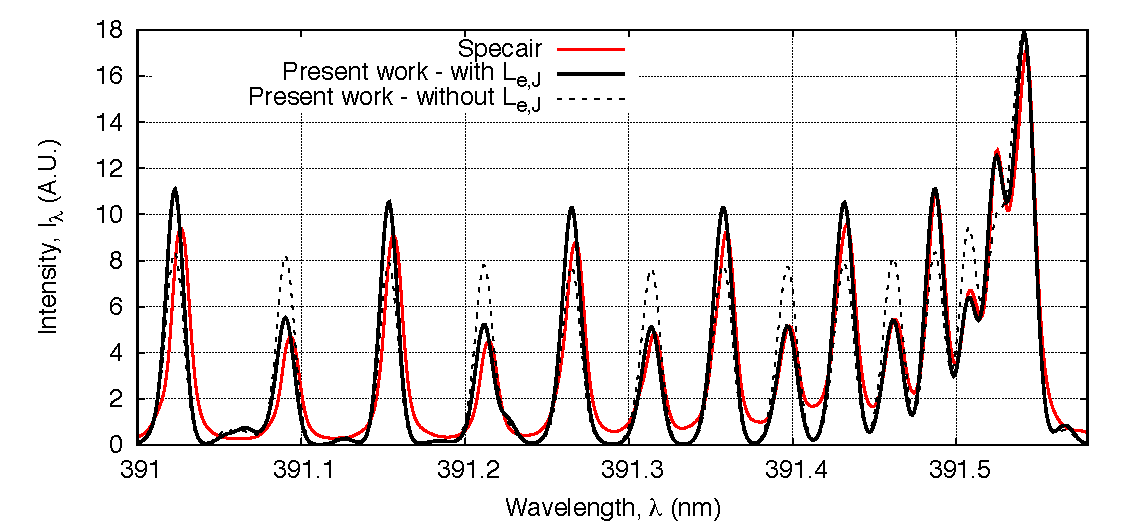
\includegraphics[width=\linewidth]{figures/spectral-modelling/N2_plus-FirstNeg-intensity_spectra_V_specair.pdf}
 \caption{Comparison of intensity spectra for the N$_2^+$ First Negative 0-0 band head calculated with and without $L_{e,J}$.}
 \label{fig:N2_plus_Vs_specair}
\end{figure}


\subsubsection{Maximum vibrational and rotational quantum numbers}

% in practice we are going to use the maximum vibrational quantum numbers provided with the ETM's, and estimate the maximum rotational quantum numbers

When calculating the electronic partition functions in Equation~\ref{eq:Q_i-mol}, the summation over the vibrational and rotational levels must be truncated at $v_\text{max}$ and $J_\text{max}$ respectively.
The strategy for determining these parameters described by Babou \textit{et al.}~\cite{BRP+2009b} is adopted.
The maximum vibrational quantum number  $v_\text{max}$ is the last that has energy within the dissociation limit referenced from the minimum of the levels potential curve:

\begin{equation}
 G_{v_\text{max}} \leq D \text{ \hspace{1cm} and \hspace{1cm} } G_{v_\text{max}+1} > D
\end{equation}

For some electronic states the vibrational energy begins to drop before the dissociation limit is reached\footnote{It should be noted this is not a physical phenomena, but rather an error due to extrapolation of spectroscopic data by the Dunham expansion}; the maximum vibrational quantum number in these cases are taken as the last level within the turning point:

\begin{equation}
 \frac{\partial G_{v_\text{max}}}{ \partial v } \geq 0 \text{ \hspace{1cm} and \hspace{1cm} }  \frac{\partial G_{v_\text{max}+1}}{ \partial v } \leq 0
\end{equation}

For each permitted vibrational level $v \leq v_\text{max}$ a maximum rotational quantum number $J_\text{max}$ must be determined.
This is achieved by considering the last rotational level that remains within the potential energy curve:

\begin{equation}
 G_v + F_{J_\text{max}} \leq V_{J_\text{max}} ( r_\text{max}  ) \text{ \hspace{0.6cm} and \hspace{0.6cm} } G_v + F_{J_\text{max}+1} > V_{J_\text{max}+1} ( r_\text{max} )
\end{equation}

The potential energy curve is the sum of the Morse and centrifugal potentials:

\begin{equation}
 V_J ( r ) = D \left [ 1 - \text{~exp} \left ( - 2 \beta \frac{r - r_e}{r_e} \right ) \right ]^2 + B_e \left ( \frac{r_e}{r} \right )^2 J ( J + 1 )
\end{equation}

\noindent where $r_e$ is the location of potential minimum and $\beta$ is:

\begin{equation}
 \beta = \frac{\omega_e}{4 \sqrt{B_e D}} \text{ . }
\end{equation}

\noindent $r_\text{max}$ is the location of the potential maximum after the potential minimum, and is therefore found when:

\begin{equation}
 \frac{ \partial V_J ( r_\text{max} )}{\partial r} = 0 \text{ \hspace{1cm} and \hspace{1cm} }   \partial^2 \frac{V_J ( r_\text{max})}{\partial r^2} < 0
\end{equation}

\subsubsection{Rovibronic energies}

The energy of a rovibronic level is comprised of electronic $\mathrm{T}_e$, vibrational $G_v$ and rotational $F_J$ contributions.
The unperturbed electronic term energies of diatomic species are available directly from the literature (\textit{e.g.} Reference~\cite{HH_NIST}).
In contrast, the vibrational $G_v$ and rotational $F_J$ energies are calculated from expressions derived via quantum mechanics.
The energy of vibrational level $v$ is calculated by the Dunham expansion which accounts for rigid rotation and anharmonic oscillations:

\begin{equation}
 G_v = \omega_e ( v + \frac{1}{2} ) - \omega_e x_e ( v + \frac{1}{2} )^2 + \omega_e y_e ( v + \frac{1}{2} )^3 + \omega_e z_e ( v + \frac{1}{2} )^4 + ... \label{eq:G_v}
\end{equation}

\noindent where $\omega_e$,  $\omega_e x_e$, $\omega_e y_e$ and $\omega_e z_e$ are the Dunham coefficients\footnote{Although the Dunham expansion is an infinite series, typically only the first 3 or 4 coefficients are available in the literature~\cite{HH_1979}.}.
The $\omega_e ( v + \frac{1}{2} )$ term represents the contribution from purely harmonic vibration, whilst the higher order terms represent anharmonic corrections.
Whilst the anharmonic corrections are neglected for the thermodynamic model, they must be retained for the spectral radiation model in order to produce a high fidelity spectra.

\par

The appropriate expression for the rotational energy is dependent on the coupling case the transition is being modelled by.
For Hund's case (a) the fine molecular structure is not considered, and the rotational energy is only a function of the rotational quantum number $J=N$ only:

\begin{equation}
% F_J = B_v J ( J + 1 ) + (A - B_v) \Lambda^2 - D_v J^2 ( J + 1 )^2 \text{ , } \label{eq:F_J_HundA}
 F_J = B_v J ( J + 1 ) - D_v J^2 ( J + 1 )^2 \text{ , } \label{eq:F_J_HundA}
\end{equation}

\noindent where,

\begin{eqnarray}
 B_v &=& B_e ( v + \frac{1}{2} ) - \alpha_e ( v + \frac{1}{2} )^2 + .... \text{ , } \label{eq:B_v} \\
 D_v &=& D_e ( v + \frac{1}{2} ) + \beta_e ( v + \frac{1}{2} )^2 + .... \text{ , } \label{eq:D_v}
\end{eqnarray}

\noindent and $B_e$ and $D_e$ are coupling constants for the electronic state which are also tabulated in the literature.

\par

For a doublet state belonging to Hund's case (b) ($\Sigma^2$ -- $\Sigma^2$ transition) separate expressions are required for the two spin split states:

\begin{eqnarray}
 F_{K=J-1/2} &=& B_v K ( K + 1 ) - D_v K^2 ( K + 1 )^2 + \frac{1}{2} \gamma K  \text{ , } \label{eq:F_K_1_HundB} \\
 F_{K=J+1/2} &=& B_v K ( K + 1 ) - D_v K^2 ( K + 1 )^2 - \frac{1}{2} \gamma \left ( K + 1 \right )  \text{ , } \label{eq:F_K_2_HundB}
\end{eqnarray}

\noindent where $\gamma$ is the spin splitting constant for the vibrational band.
In the present work the $\gamma$ values for the CN Violet transition are those presented by Prasad and Bernath~\cite{PB1992}.
The energies of the two spin split components for doublet states belonging to the intermediate (a)-(b) are:

\begin{eqnarray}
 F_{K=J-1/2} &=& B_v \left [ K ( K + 1 ) - \Lambda^2 + \frac{Y \left ( 4 - Y \right )}{8 ( K + 1 )} \Lambda^2 \right ] - D_v ( K + \frac{1}{2} )^4  \text{ , } \label{eq:F_K_1_HundAB} \\
 F_{K=J+1/2} &=& B_v \left [ K ( K + 1 ) - \Lambda^2 + \frac{Y \left ( 4 - Y \right )}{8 K} \Lambda^2 \right ] - D_v ( K + \frac{1}{2} )^4  \text{ , } \label{eq:F_K_2_HundAB}
\end{eqnarray}

\noindent where $Y = A / B_v$.
For triplet states belonging to the intermediate (a)-(b) case, the energies of the three spin split components are:

\begin{eqnarray}
 F_{J=K+1} &=&  B_v \left [ J ( J + 1 ) - \sqrt{Z_1} - 2 Z_2 \right ] - D_v \left ( J - \frac{1}{2} \right )^4 \label{eq:F_J_1_HundAB_triplet} \\
 F_{J=K} &=&  B_v \left [ J ( J + 1 ) + 4 Z_2 \right ] - D_v \left ( J + \frac{1}{2} \right )^4 \label{eq:F_J_2_HundAB_triplet} \\
 F_{J=K-1} &=&  B_v \left [ J ( J + 1 ) + \sqrt{Z_1} - 4 Z_2 \right ] - D_v \left ( J + \frac{3}{2} \right )^4 \label{eq:F_J_3_HundAB_triplet}
\end{eqnarray}

\noindent where $Z_1$ and $Z_2$ are calculated as:

\begin{eqnarray}
 Z_1 = \Lambda^2 Y \left ( Y - 4 \right ) + \frac{4}{3} + 4 J \left ( J + 1 \right ) \\
 Z_2 = \frac{1}{3Z_1} \left [ \Lambda^2 Y \left ( Y - 1 \right ) - \frac{4}{9} - 2 J \left ( J + 1 \right ) \right ]
\end{eqnarray} 

\subsubsection{Radiative transition probabilities}
\label{sec:RTP}

% - describe Hund coupling cases
% - describe the transition groups we will consider, and the relevent energy, HLF expressions

The radiative transition probability $A_{ul}$ given in Equations~\ref{eq:diatomic_j_nu_ul} and~\ref{eq:diatomic_kappa_nu_lu} is calculated as:

\begin{equation}
 A_{ul} = \frac{64 \pi^4 \nu_{ul}^3}{3 h c^3} \frac{ \left ( a_0 e \right )^2 \left ( R_e^{v_u v_l} \right )^2 }{ \left ( 2 - \delta_{0,\Lambda_u} \right ) \left ( 2 S + 1 \right ) } \frac{S^{J_u}_{J_l}}{2 J_u + 1}
\end{equation}
% all constants are in CGS units

\noindent where $\nu_{ul}$ is the transition frequency in Hz, $\left ( a_0 e \right )^2 \left ( R_e^{v_u v_l} \right )^2$ is the square of the electronic-vibrational transition moment expressed in statcoulombs and $S^{J_u}_{J_l}$ is the H\"{o}nl--London factor for the rotational transition.
The electronic-vibrational transition moments proposed by Chauveau \textit{et al.}~\cite{CPR+2002} and Babou \textit{et al.}~\cite{BRP+2009} have been implemented in the present work.
These two datasets were selected as they represent the most recent set of transition moments calculated with up-to-date electronic transition moment functions and a consistent treatment of the potential energy function (an RKR potential was used for all species).
These diatomic systems and the respective references are summarised in Table~\ref{tab:diatomic_systems}.
Note that the additional systems considered by Hyun~\cite{hyun_phd} that are not covered in References~\cite{CPR+2002,BRP+2009} have also been included.

% The data of Reference~\cite{CPR+2002} and~\cite{BRP+2009} have been preferenced over those of Reference~\cite{hyun_thesis} due to the former encompassing a wider range of vibrational bands to a higher degree of precision.
% Furthermore, the methodology used in calculating the transition moments are described in full in Reference~\cite{CPR+2002} and~\cite{BRP+2009} while those in Reference~\cite{hyun_thesis} are not.
% -> What about Mario Lino da Silva's work?
% NOTES: - some systems (N2 VK etc) in the SPRADIAN07 code are NOT in Hyun's thesis - the data is probably dubious, so omit them I guess
%                 - CN Red ETM's from Babou et al is much stronger (x10) than those from SPRADIAN07

 \begin{center}
 \begin{footnotesize}
  \tablefirsthead{%
  \hline \hline Diatomic Species   &  System name                                 & Transition designation                                                  & Included bands                                                           & $ R_e^{v_u v_l}$ Reference\\
                                                          &                                                      &                                                                                           & (0 : $v_{u,\text{max}}$; 0 : $v_{l,\text{max}}$ ) \\
  \hline}
 \tablehead{%
  \hline
  \multicolumn{5}{l}{\small\sl table continued from previous page...}\\
  \hline \hline Diatomic Species   &  System name                                 & Transition designation                                                  & Included bands                                                           & $ R_e^{v_u v_l}$ Reference\\
                                                &                                                      &                                                                                           & (0 : $v_{u,\text{max}}$; 0 : $v_{l,\text{max}}$ ) \\
  \hline}
 \tabletail{%
  \hline
  \multicolumn{5}{l}{\small\sl table continued on next page...}\\
  \hline \vspace{0.5cm} \\}
 \tablelasttail{%
  \hline
  }
 \topcaption{Diatomic systems considered in the present work.}
 \label{tab:diatomic_systems}
 \begin{supertabular*}{1.0\textwidth}{ccccc}
                           CO               & Infrared                                       & $X^1 \Sigma^+$ -- $X^1 \Sigma^+$                           & (0:50; 0:50)                               & \cite{BRP+2009} \\
                                                & Fourth--Positive                        &             $A^1 \Pi$ -- $X^1 \Sigma^+$                            & (0:23; 0:50)                               & \cite{BRP+2009} \\
                                                & BX (Hopfield--Birge)                & $B^1 \Sigma^+$ -- $X^1 \Sigma^+$                            & (0:2; 0:50)                               & \cite{BRP+2009} \\
                                                & CX                                               & $C^1 \Sigma^+$ -- $X^1 \Sigma^+$                            & (0:9; 0:9)                                 & \cite{hyun_phd} \\
                                                & EX                                               & $E^1 \Pi$ -- $X^1 \Sigma^+$                                         & (0:5; 0:5)                                 & \cite{hyun_phd} \\
                                                & FX                                               & $F^1 \Sigma^+$ -- $X^1 \Sigma^+$                             & (0:1; 0:0)                                 & \cite{hyun_phd} \\
                                                & GX                                               & $G^1 \Pi$ -- $X^1 \Sigma^+$                                        & (0:2; 0:0)                                 & \cite{hyun_phd} \\
                                                & Third--Positive                          & $b^3 \Sigma^+$ -- $a^3 \Pi$                                         & (0:2; 0:18)                               & \cite{BRP+2009} \\
\\
                           CO$^+$      & Comet--tail                                & $A^2 \Pi_i$ -- $X^2 \Sigma^+$                                      & (0:33; 0:31)                               & \cite{BRP+2009} \\
                                                & Baldet--Johnson                      & $B^2 \Sigma^+$ -- $A^2 \Pi_i$                                      & (0:33; 0:50)                               & \cite{BRP+2009} \\
                                                & First Negative                           & $B^2 \Sigma^+$ -- $X^2 \Sigma^+$                             & (0:22; 0:35)                               & \cite{BRP+2009} \\
\\
                           CN               & Red                                            & $A^2 \Pi_i$ -- $X^2 \Sigma^+$                                      & (0:38; 0:34)                               & \cite{BRP+2009} \\
                                                & Violet                                         & $B^2 \Sigma^+$ -- $X^2 \Sigma^+$                             & (0:25; 0:36)                               & \cite{BRP+2009} \\
                                                & LeBlanc                                    & $B^2 \Sigma^+$ -- $A^2 \Pi_i$                                      & (0:25; 0:38)                               & \cite{BRP+2009} \\
\\
                           C$_2$        & Phillips                                      & $A^1 \Pi_u$ -- $X^1 \Sigma_g^+$                                & (0:35; 0:21)                               & \cite{BRP+2009} \\
                                               & Mulliken                                    & $D^1 \Sigma_u^+$ -- $X^1 \Sigma_g^+$                    & (0:22; 0:21)                               & \cite{BRP+2009} \\
                                               & Delandres--D'Azambuja        & $C^1 \Pi_g$ -- $A^1 \Pi_u$                                            & (0:9; 0:32)                               & \cite{BRP+2009} \\
                                               & Ballik--Ramsay                        & $b^3 \Sigma_g^-$ -- $a^3 \Pi_u$                                  & (0:41; 0:39)                               & \cite{BRP+2009} \\
                                               & Swan                                         & $d^3 \Pi_g$ -- $a^3 \Pi_u$                                              & (0:18; 0:33)                               & \cite{BRP+2009} \\
                                               & Fox--Herzberg                         & $e^3 \Pi_g$ -- $a^3 \Pi_u$                                              & (0:15; 0:35)                               & \cite{BRP+2009} \\
                                               & Freymark                                  & $E_1 \Sigma_g^+$ -- $A^1 \Pi_u$                                 & (0:6; 0:4)                                 & \cite{hyun_phd} \\
\\
                           N$_2$       & First--Positive                           & $B^3 \Pi_g$ -- $A^3 \Sigma_u^+$                                 & (0:21; 0:16)                               & \cite{CPR+2002} \\
                                              & Second--Positive                     & $C^3 \Pi_u$ -- $B^3 \Pi_g$                                             & (0:4; 0:21)                               & \cite{CPR+2002} \\
                                              & Birge--Hopfield 1                     & $b^1 \Pi_u$ -- $X^1 \Sigma_g^+$                                  & (0:19; 0:15)                               & \cite{CPR+2002} \\
                                              & Birge--Hopfield 2                     & $b^{\prime 1} \Sigma_u^+$ -- $X^1 \Sigma_g^+$       & (0:28; 0:15)                               & \cite{CPR+2002} \\
                                              & Carroll--Yoshino                      & $c^{\prime 1}_4 \Sigma_u^+$ -- $X^1 \Sigma_g^+$   & (0:8; 0:15)                               & \cite{CPR+2002} \\
                                              & Worley--Jenkins                      & $c^1_3 \Pi_u$ -- $X^1 \Sigma_g^+$                               & (0:4; 0:15)                               & \cite{CPR+2002} \\
                                              & Worley                                       & $o^1_3 \Pi_u$ -- $X^1 \Sigma_g^+$                               & (0:4; 0:15)                               & \cite{CPR+2002} \\
\\
                           N$_2^+$  & Meinel                                      & $A^2 \Pi_u$ -- $X^2 \Sigma_g^+$                                     & (0:27; 0:21)                               & \cite{CPR+2002} \\
                                              & First--Negative                        & $B^2 \Sigma_u^+$ -- $X^2 \Sigma_g^+$                        & (0:8; 0:21)                               & \cite{CPR+2002} \\
                                              & Second--Negative                 & $C^2 \Sigma_u^+$ -- $X^2 \Sigma_g^+$                        & (0:6; 0:21)                               & \cite{CPR+2002} \\
\\
                           NO             & $\gamma$                                & $A^2 \Sigma^+$ -- $X^2 \Pi_r$                                         & (0:8; 0:22)                               & \cite{CPR+2002} \\
                                              & $\beta$                                      & $B^2 \Pi_r$ -- $X^2 \Pi_r$                                                 & (0:37; 0:22)                               & \cite{CPR+2002} \\
                                              & $\delta$                                     & $C^2 \Pi_r$ -- $X^2 \Pi_r$                                                 & (0:9; 0:22)                               & \cite{CPR+2002} \\
                                              & $\epsilon$                                 & $D^2 \Sigma^+$ -- $X^2 \Pi_r$                                        & (0:5; 0:22)                               & \cite{CPR+2002} \\
                                              & $\gamma^\prime$                   & $E^2 \Sigma^+$ -- $X^2 \Pi_r$                                        & (0:4; 0:22)                               & \cite{CPR+2002} \\
                                              & $\beta^\prime$                         & $B^{\prime 2} \Delta$ -- $X^2 \Pi_r$                                & (0:6; 0:22)                               & \cite{CPR+2002} \\
                                              & 11,000 \AA                                & $D^2 \Sigma^+$ -- $A^2 \Sigma^+$                                & (0:5; 0:8)                               & \cite{CPR+2002} \\
                                              & Infrared                                      & $X^2 \Pi_r$ -- $X^2 \Pi_r$                                                  & (0:22; 0:22)                               & \cite{CPR+2002} \\
\\
                           O$_2$       & Schumann--Runge                 & $B^3 \Sigma_u^-$ -- $X^3 \Sigma_g^-$                         & (0:19; 0:21)                               & \cite{CPR+2002} \\
 \end{supertabular*}
  \end{footnotesize}
 \end{center}


\par

The H\"{o}nl--London factor describes the strength of the rotational lines.
The sum of all H\"{o}nl--London factors ending in a given lower rotational state must equate to the total degeneracy of the level:

\begin{equation}
 \sum_{J_u} S^{J_u}_{J_l} = \left ( 2 - \delta_{0,\Lambda_u+\Lambda_l} \right ) \left ( 2 S_l + 1 \right ) \left ( 2 J_l + 1 \right )
\end{equation}

The selection of the H\"{o}nl--London factors therefore depends on the transition type under consideration.
The H\"{o}nl--London factors for all transitions belonging to Hund's case (a) are shown in Table~\ref{tab:HundA_HLF}.

\begin{table}[h]
 \center
 \caption{H\"{o}nl--London factors for Hund's case (a).}
 \label{tab:HundA_HLF}
 \begin{tabular*}{1.0\textwidth}{cccc}
  \hline Branch                           & $S^{J_u}_{J_l}$ for $\Lambda_u=\Lambda_l=0$ & $S^{J_u}_{J_l}$ for $\Delta \Lambda = 0$                                                                                  & $S^{J_u}_{J_l}$ for $\Delta \Lambda = \pm 1$ \\
  \hline  P ($\Delta J = +1$)     & $J_u + 1$                                                                      & $\frac{ \left ( J_u + 1 + \Lambda_u \right ) \left ( J_u + 1 - \Lambda_u \right ) }{ J_u + 1 }$  & $\frac{ \left ( J_u + 1 \mp \Lambda_u \right ) \left ( J_u + 2 \mp \Lambda_u \right ) }{ 2 \left ( J_u + 1 \right ) }$ \\
              Q ($\Delta J =  0$)      &0                                                                                       & $\frac{ \left ( 2 J_u + 1 \right ) \Lambda_u^2 }{ J_u \left ( J_u + 1 \right )  }$                           & $\frac{ \left ( J_u \pm \Lambda_u \right ) \left ( J_u + 1 \mp \Lambda_u \right ) \left ( 2 J_u + 1 \right ) }{ 2  J_u \left ( J_u + 1 \right ) }$ \\
              R  ($\Delta J = -1$)    & $J_u$                                                                             & $\frac{ \left ( J_u + \Lambda_u \right ) \left ( J_u - \Lambda_u \right ) }{ J_u }$                      & $\frac{ \left ( J_u \pm \Lambda_u \right ) \left ( J_u - 1 \pm \Lambda_u \right ) }{ 2 J_u }$ \\
  \hline
 \end{tabular*}
\end{table}

For $^2\Sigma$--$^2\Sigma$ transitions belonging to Hund's case (b), the H\"{o}nl--London factors presented by Mulliken~\cite{Mulliken31} are implemented, Table~\ref{tab:HundB_HLF}.

\begin{table}[h]
 \center
 \caption{H\"{o}nl--London factors for $^2\Sigma$--$^2\Sigma$ transitions belonging to Hund's case (b).}
 \label{tab:HundB_HLF}
 \begin{tabular*}{0.3\textwidth}{cc}
  \hline Branch                          & $S^{J_u}_{J_l}$ \\
  \hline  R ($\Delta J = +1$)    & $\frac{ \left ( J_l + 1 \right )^2 - \frac{1}{4} }{J_l + 1}$ \\
              Q ($\Delta J =   0$)    & $\frac{ \left ( 2 J_l + 1 \right )}{4 J_l \left ( J_l + 1 \right ) }$ \\
              P  ($\Delta J = -1$)    & $\frac{ J_l^2 - \frac{1}{4} }{J_l}$ \\
  \hline
 \end{tabular*}
\end{table}

For the parallel doublet transitions modelled by the intermediate (a)-(b) case, the H\"{o}nl--London factors used by Arnold \textit{et al.}~\cite{Arn69} in the RAD/EQUIL code are implemented, Table~\ref{tab:HundAB_HLF}.
In this table the upper sign corresponds with upper listed branch and $U$ is defined as:

\begin{equation}
 U = \left [ Y^2 - 4 Y + ( 2 J + 1 ) \right ] \text{ , }
\end{equation}

\noindent where  $Y = A / B_v$.
 
\begin{table}[h]
 \center
 \caption{H\"{o}nl--London factors for $^2\Pi$--$^2\Sigma$ transitions belonging to Hund's intermediate (a)-(b) case.}
 \label{tab:HundAB_HLF}
 \begin{tabular*}{0.7\textwidth}{ccc}
  \hline \multicolumn{2}{c}{Branch}                                                                                                                                                                     & $S^{J_u}_{J_l}$ \\
              $^2\Pi$ $\Rightarrow$ $^2\Sigma$                      &           $^2\Sigma$ $\Rightarrow$ $^2\Pi$                                                   & \\
  \hline  $\begin{array}{c} P_2 \\ ^OP_{1 2} \end{array}$ & $\left . \begin{array}{c} R_2 \\ ^S R_{2 1} \end{array} \right \rbrace$     & $\frac{(2 J_u + 1)^2 \pm (2 J_u + 1 ) U_u ( 4 J_u^2 + 4 J_u + 1 - 2Y_u )}{16 ( J_u +1 )}$ \\ 
              $\begin{array}{c} ^Q P_{2 1} \\ P_1 \end{array}$ & $\left . \begin{array}{c} Q R_{1 2} \\ R_1 \end{array} \right \rbrace$     & $\frac{(2 J_u + 1)^2 \mp (2 J_u + 1 ) U_u ( 4 J_u^2 + 4 J_u -7 + 2Y_u )}{16 ( J_u +1 )}$ \\
              $\begin{array}{c} Q_2 \\ ^P Q_{1 2} \end{array}$ & $\left . \begin{array}{c} Q_2 \\ ^R Q_{2 1} \end{array} \right \rbrace$   & $\frac{(2 J_u + 1) \left [ ( 4 J_u^2 + 4 J_u - 1 ) \pm U_u ( 8 J_u^3 + 12 J_u ^2 - 2 J_u + 1 - 2 Y_u ) \right ]}{16 J_u ( J_u +1 )}$ \\ 
              $\begin{array}{c} ^R Q_{2 1} \\ Q_1 \end{array}$ & $\left . \begin{array}{c} ^P Q_{1 2} \\ Q_1 \end{array} \right \rbrace$   & $\frac{(2 J_u + 1) \left [ ( 4 J_u^2 + 4 J_u - 1 ) \mp U_u ( 8 J_u^3 + 12 J_u ^2 - 2 J_u - 7 + 2 Y_u ) \right ]}{16 J_u ( J_u +1 )}$ \\ 
              $\begin{array}{c} R_2 \\ ^Q R_{1 2} \end{array}$ & $\left . \begin{array}{c} P_2 \\ ^Q P_{2 1} \end{array} \right \rbrace$    & $\frac{(2 J_u + 1)^2 \pm (2 J_u + 1 ) U_u ( 4 J_u^2 + 4 J_u -7 + 2Y_u )}{16 J_u}$ \\
              $\begin{array}{c} ^S R_{2 1} \\ R_1 \end{array}$ & $\left . \begin{array}{c} ^O P_{1 2} \\ P_1 \end{array} \right \rbrace$    & $\frac{(2 J_u + 1)^2 \mp (2 J_u + 1 ) U_u ( 4 J_u^2 + 4 J_u + 1 - 2Y_u )}{16 J_u}$ \\ 
  \hline
 \end{tabular*}
\end{table}

\subsubsection{Spectral distribution function }

The spectral distribution function for diatomic lines is the same as that described for monatomic lines in Section~\ref{sec:monatomic_transitions}, however resonance broadening is not considered.
The trends observed for the monatomic linewidths in Figures~\ref{fig:air-linewidths} and~\ref{fig:mars-linewidths} are therefore also applicable to the diatomic linewidths.

\par

Figures~\ref{fig:atomic-EvLE} and~\ref{fig:atomic-IvLE} compare the sensitivity of diatomic bound-bound emissive power density and intensity for a 10\,cm slab of atmospheric pressure equilibrium air to the diatomic line cut-off limit.
The line cut-off limit $\Delta \nu_\text{limit}$ has been normalised by the voigt HWHM $\gamma_V$, and the emissive power density and intensity are normalised by the respective values at $\Delta \nu_\text{limit} = 1,000 \gamma_V$.
Both the emissive power density and intensity are reasonably well described with $\Delta \nu_\text{limit} / \gamma_V \geq 10$, although significant improvement is achieved with $\Delta \nu_\text{limit} / \gamma_V \geq 100$.
In the present work the diatomic line cut-off limit is set to $\Delta \nu_\text{limit} = 10 \gamma_V$ as a compromise between accuracy and efficiency.

\begin{figure}[h]
 \centering
 \subfloat[Emissive power density]{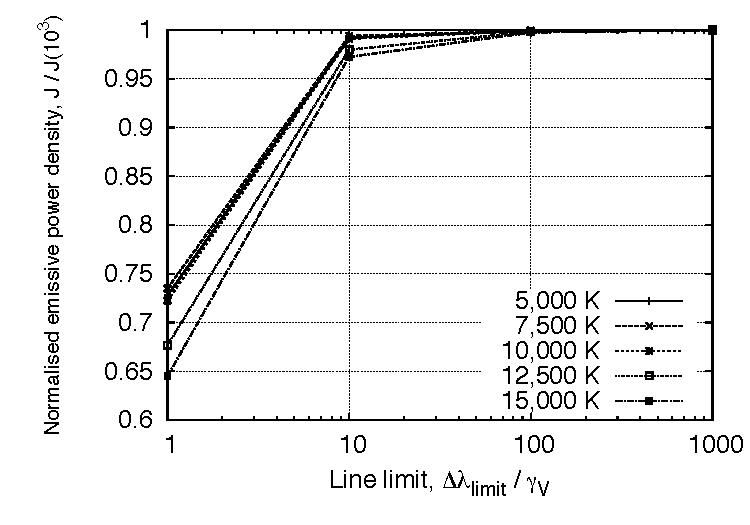
\includegraphics[width=0.5\linewidth]{figures/spectral-modelling/diatomic-EvLineExtent.pdf} \label{fig:diatomic-EvLE}}
 \subfloat[Intensity]{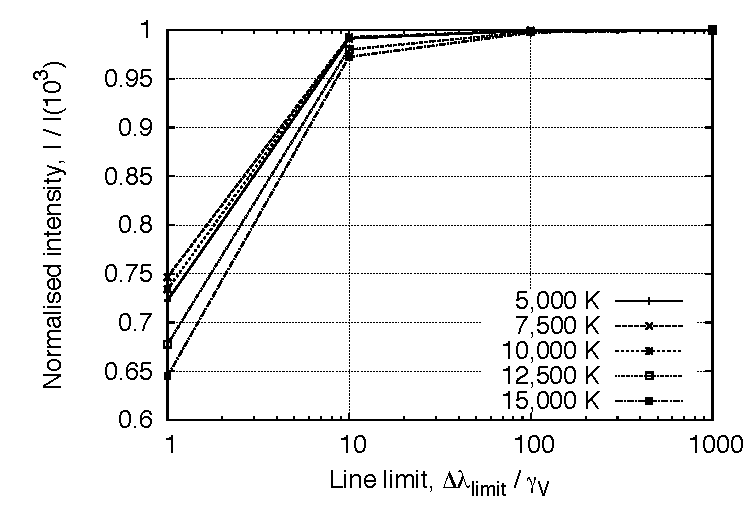
\includegraphics[width=0.5\linewidth]{figures/spectral-modelling/diatomic-IvLineExtent.pdf} \label{fig:diatomic-IvLE}}
 \caption{Sensitivity of diatomic bound-bound emissive power density and intensity for a 10\,cm slab of equilibrium air to the diatomic line cut-off limit ($p=1$\,atm).}
 \label{fig:diatomic_LE_sensitivity}
\end{figure}

\subsubsection{Comparison with SPRADIAN07}

As was done for monatomic bound-bound transitions, comparisons with the SPRADIAN07 code~\cite{hyun_phd} have been made in order to verify the calculation of diatomic bound-bound spectral coefficients.
For this purpose, the electronic-vibrational transition moments presented by Hyun~\cite{hyun_phd} are used so that both codes are using the same fundamental data.
Also, the line-alternation factor $L_{e,j}$ for homonuclear molecules is omitted and the CN Violet system is modelled via Hund's case (a) for consistency with SPRADIAN07.
The test case consists of a 10\,cm slab of gas with temperature $T=10,000$\,K and pressure $p=1$\,atm.
The number density of each radiator is $1 \times 10^{16}$\,cm$^{-3}$, the electron number density is also $1 \times 10^{16}$\,cm$^{-3}$ and total number density is $2.2 \times 10^{17}$\,cm$^{-3}$.
For each radiator, the emissive power density $J$ (W/cm$^3$) and intensity $I$ (W/cm$^2$) is calculated in the spectral range $ 50 \leq \lambda \leq 2,000$\,nm with 1,950,000 equidistant frequency intervals.  

\par

Table~\ref{tab:spradian_diatom_compare} summarises the comparison between the SPRADIAN07 code~\cite{hyun_phd} and the present work for diatomic bound-bound transitions.
The agreement for both emissive power density and intensity is within 5\% for all the diatomic radiators considered, with key species such as C$_2$, CN and N$_2^+$ agreeing within 2\%.
Figures~\ref{fig:CN-violet-emission},~\ref{fig:CN-violet-abs} and~\ref{fig:CN-violet-intensity} presents the emission coefficient, absorption coefficient and intensity spectra for the CN Violet 0-0 band-head in the spectral range $387 \leq \lambda \leq 388.5$\,nm.
Calculations using the vibration-electronic transition moments of both Hyun~\cite{hyun_phd} and Babou \textit{et al.}~\cite{BRP+2009} are presented.
The SPRADIAN07 data exhibits lower troughs between lines, indicating the line-widths are slightly smaller.
While the cumulative emission for the Hyun $R_e$ case shows only a 0.4\% difference with SPRADIAN07, the differences in line shape between the two coefficient spectrums result in a slightly higher difference in cumulative intensity of 0.6\%.
Using the transition moments of Babou results in 10\% higher intensity, and additional lines appear as a consequence of Babou considering more bands than Hyun.
Overall, the agreement with SPRADIAN07 is very good and verifies the implementation of the equations describing bound-bound transitions in the present work.

\begin{table}[h]
 \small
 \center
 \caption{Comparison of datomic bound-bound model from the present work with the SPRADIAN07 code~\cite{hyun_phd}.}
 \label{tab:spradian_diatom_compare}
 \begin{tabular*}{1.0\textwidth}{ccccccc}
  \hline Species                          & \multicolumn{3}{c}{Emissive power density, $J$ (W/cm$^3$)}        & \multicolumn{3}{c}{Intensity, $I$ (W/cm$^2$)}      \\
                                                      & SPRADIAN07 & Present work  & Difference (\%)                     & SPRADIAN07 & Present work & Difference (\%) \\
  \hline  
                  C$_2$                       & 1342             & 1328                 & -1.06                                      & 772.1             & 768.5              & -0.46 \\
                  CN                             & 1079             & 1075                 & -0.42                                      & 470.6              & 473.6             &  0.62 \\
                  CO                             & 584.3            & 560.8                & -4.03                                       & 181.2             & 177.1             & -2.32 \\
                  N$_2$                       & 8.85              & 8.48                  & -4.08                                       & 5.61                & 5.42               & -3.60 \\
                  N$_2^+$                  & 1235             & 1244                 & 0.71                                         & 646.8             & 655.7            & 1.36 \\
                  NO                             & 112.0            & 109.0                & -2.67                                       & 84.44             & 82.75             & -2.04 \\
                  O$_2$                      & 78.79             & 82.31                & 4.47                                        & 61.12             & 62.51             &  2.22 \\
  \hline
 \end{tabular*}
\end{table}

\begin{figure}[p]
 \centering
 \subfloat[Emission]{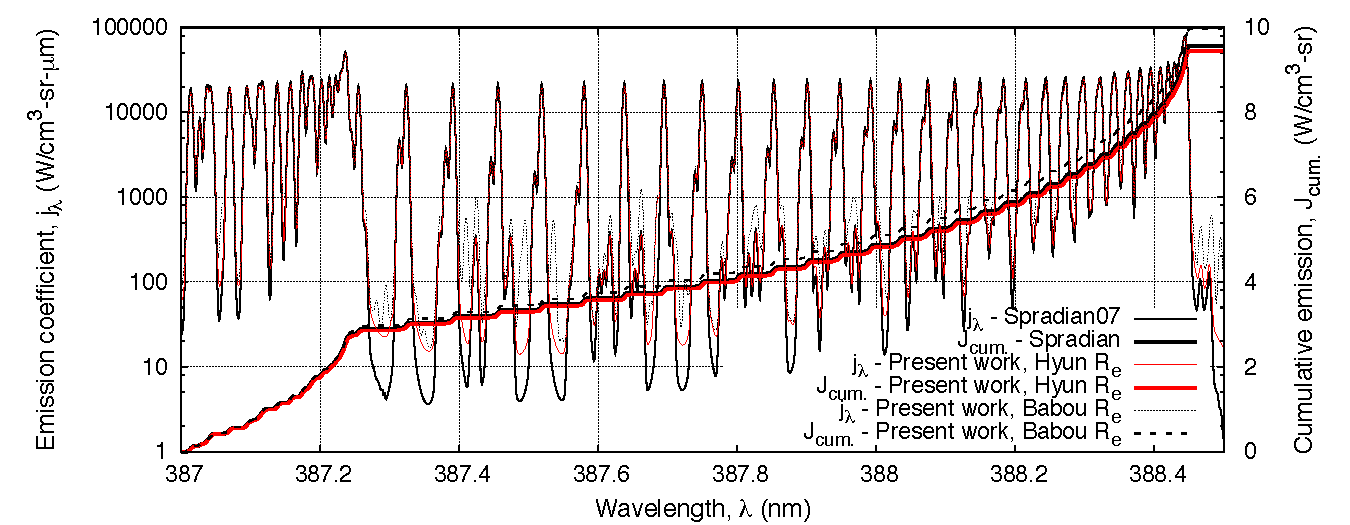
\includegraphics[width=1.0\linewidth]{figures/spectral-modelling/CN-violet-emission.pdf}  \label{fig:CN-violet-emission}} \\
 \subfloat[Absorption]{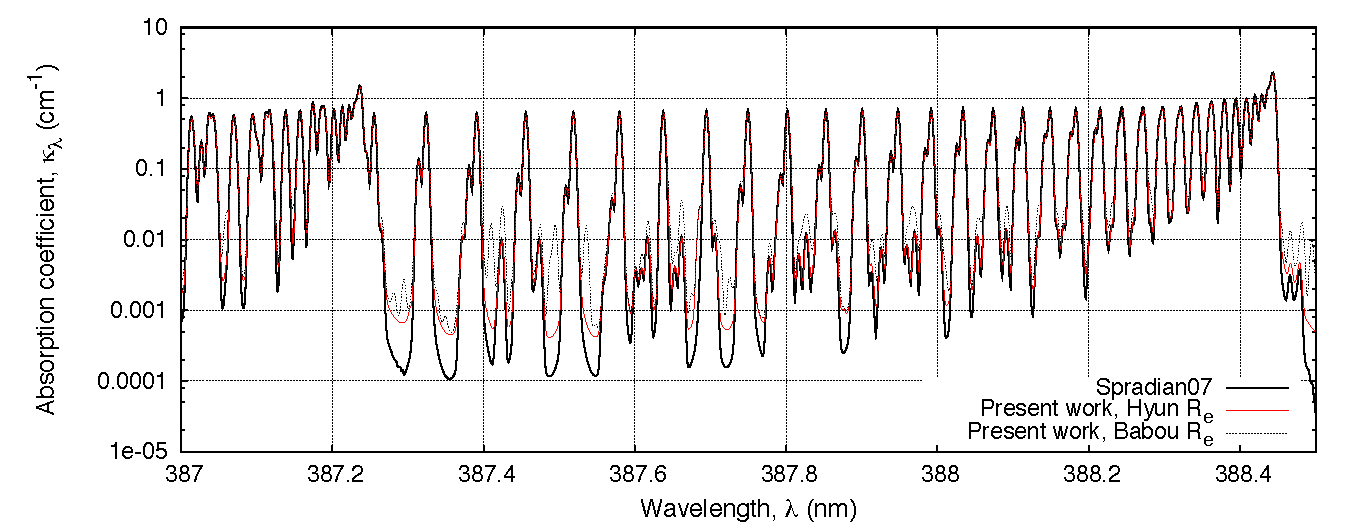
\includegraphics[width=1.0\linewidth]{figures/spectral-modelling/CN-violet-abs.pdf}  \label{fig:CN-violet-abs}} \\
 \subfloat[Spectral and cumulative intensity]{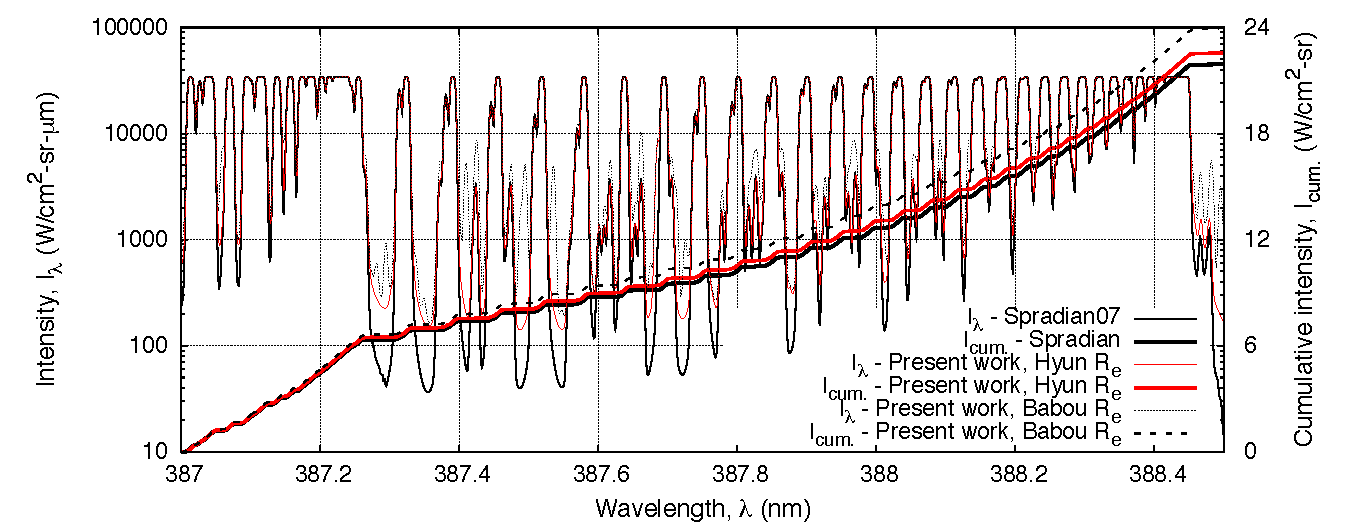
\includegraphics[width=1.0\linewidth]{figures/spectral-modelling/CN-violet-intensity.pdf}  \label{fig:CN-violet-intensity}}
 \caption{Comparison between SPRADIAN07 and the present work for the spectra of the CN Violet 0-0 band-head in the range $387 \leq \lambda \leq 388.5$\,nm.}
\end{figure}

\subsubsection{Comparison of transition moment data sets}

As the transition moments of Chauveau \textit{et al.}~\cite{CPR+2002} and Babou \textit{et al.}~\cite{BRP+2009} and are being used in preference to the Hyun~\cite{hyun_phd} data set, it is appropriate to compare the two.
Table~\ref{tab:EM2C_diatom_compare} presents a comparison of the diatomic species integrated emission and intensities using the Babou\footnote{Here `Babou' denotes the set of transition moments described in Table~\ref{tab:diatomic_systems}, which are mainly from Babou \textit{et al.}~\cite{BRP+2009}.} and Hyun transition moments.
While C$_2$, CN, CO, N$_2^+$ and O$_2$ show only minor deviations of 20\% or less, NO and N$_2$ emission are increased by 74\% and 787\% when using the Babou transition moments.

\begin{table}[h]
 \small
 \center
 \caption{Comparison of integrated emission and intensity using the transition moments of Hyun~\cite{hyun_phd} and of Babou \textit{et al.}~\cite{BRP+2009}.}
 \label{tab:EM2C_diatom_compare}
 \begin{tabular*}{0.9\textwidth}{ccccccc}
  \hline Species                          & \multicolumn{3}{c}{Emissive power density, $J$ (W/cm$^3$)}        & \multicolumn{3}{c}{Intensity, $I$ (W/cm$^2$)}      \\
                                                      &  Hyun $R_e$  & Babou $R_e$ & Difference (\%)                     & Hyun $R_e$  & Babou $R_e$ & Difference (\%) \\
  \hline  
                  C$_2$                       & 1328                 &    1479       & 11.37                                     & 768.5      &    698.6    & -10.0 \\
                  CN                             & 1075                 &    1181       &  9.91                                       & 473.6      &    569.7   &  16.9 \\
                  CO                             & 560.8                &    473.6      & -15.54                                    & 177.1       &   198.8   & 10.93  \\
                  N$_2$                       & 8.48                  &    75.25      &  787                                         & 5.42        &    27.3   & 80.2 \\
                  N$_2^+$                  & 1244                 &    1204       & -3.21                                        &  655.7     &   501.6   & -30.7 \\
                  NO                             & 109.0                &    189.9     & 74.21                                       & 82.75     &   140.86 & 41.3 \\
                  O$_2$                      & 82.31                &    99.66      & 21.08                                        & 62.51    &     76.12    & 17.9 \\
  \hline
 \end{tabular*}
\end{table}

\par

The large difference for the N$_2$ molecule warrants further investigation, especially considering Hyun uses the well regarded data of Laux~\cite{laux_1993,LK1992} for the N$_2$ transitions\footnote{The calculations for the VUV system transition moments, however, are stated by Hyun~\cite{hyun_phd} to be from Laux but are from a yet to be published source.}.
Table~\ref{tab:N2_radiation_compare} presents a comparison of the integrated emission and intensities using the Chauveau \textit{et al.}~\cite{CPR+2002} and Hyun~\cite{hyun_phd} transition moments for each system of the N$_2$ molecule.
The well known First--Positive and Second--Positive systems, which radiate in the ultraviolet spectral region, are in good agreement, whilst the remaining systems exhibit significant differences.
These systems with large differences --- Birge--Hopfield 1, Birge--Hopfield 2, Carroll--Yoshino, Worley--Jenkins and Worley --- are all vacuum ultraviolet systems.
Due to the difficulty of performing emission spectroscopy in the VUV spectral region, there has been little experimental corroboration for theoretical calculation of the transition moments for these systems.
Consequently there is a significant degree of uncertainty associated with the intensity of the N$_2$ VUV systems, and it is not uncommon for different sets of theoretical calculations to show substantial discrepancies.  
For example, Liebhart \textit{et al.} calculated the electronic transition moments for N$_2$ VUV systems via an RKR reconstruction of the potential energy surface.
Calculations of equilibrium air absorption spectra at 7,000\,K deviated by up to an order of magnitude from the results obtained by Chauveau \textit{et al.}~\cite{CPR+2002}, most notably for the strong band peaks at 95\,nm.
As the transition moments for the N$_2$ VUV systems used by Hyun~\cite{hyun_phd} are from a yet to be published source, the Chauveau \textit{et al.}~\cite{CPR+2002} data is felt to be more appropriate for the present work.

\begin{table}[h]
 \small
 \center
 \caption{Comparison of integrated emission and intensity using the transition moments from Hyun~\cite{hyun_phd} and Chauveau \textit{et al.}~\cite{CPR+2002}.}
 \label{tab:N2_radiation_compare}
 \begin{tabular*}{0.9\textwidth}{ccccccc}
  \hline N$_2$ systems             & \multicolumn{3}{c}{Emissive power density, $J$ (W/cm$^3$)}        & \multicolumn{3}{c}{Intensity, $I$ (W/cm$^2$)}      \\
                                                      &  Hyun $R_e$  & Chauveau $R_e$ & Difference (\%)                               & Hyun $R_e$  & Chauveau $R_e$ & Difference (\%) \\
  \hline  
        First--Positive                     &    0.75                &      0.83             &      -9.33                                           &    0.60               & 0.66                  &     -9.30             \\
        Second--Positive               &    1.18                &      1.18             &      -0.02                                           &    0.94               & 0.94                  &     -0.02             \\
        Birge--Hopfield 1               &  57.09                &      3.88             &       1372                                          &    29.09            & 2.77                  &      950               \\
        Birge--Hopfield 2               &    6.68                &      0.40             &        1566                                          &      4.47            & 0.32                  &      1319            \\
        Carroll--Yoshino                &    5.91                &      1.65             &        257                                            &      1.86            & 0.52                  &      259               \\
        Worley--Jenkins                &     2.07                &      0.17             &       1094                                           &      0.71            & 0.11                  &     554               \\ 
        Worley                                 &    1.58                &      0.37             &        329                                             &      0.74            & 0.23                  &     217               \\
  \hline
 \end{tabular*}
\end{table}


\subsection{Continuum transitions}
\label{sec:continuum_transitions}

In the present work the continuum transitions for atomic species and their ions are considered, whilst continuum transitions for molecular species are neglected.
Furthermore, the models for atomic continuum transitions are based on approximate curve-fits and hydrogenic assumptions.
Such a simplified treatment of continuum transitions is justified based on the:

\begin{enumerate}
 \item Low concentration of molecules and their ions for high-speed Earth and Mars entry, 
 \item Small contribution of continuum mechanisms to optically thin emission in CO$_2$--N$_2$ plasmas at temperature less than 15,000\,K~\cite{BRP+2009}, and
 \item Demonstrated efficacy of photoionisation curve-fits for N and O in high temperature air plasmas~\cite{JHS2008a}.
\end{enumerate}

This rationale, however, is not valid for the cool boundary layer surrounding an aeroshell, as at low temperatures ($T\lesssim 6000$\,K) the photoionisation and photodissociation continua of diatomic species can be significant~\cite{CDP+2003,BRP+2009}.
As a consequence, the omission of these mechanisms may lead to an underprediction of the radiative energy absorbed or emitted by the boundary layer.
In addition, photodetachment processes for negative ions are estimated to be significant at temperatures up to temperatures of 12,000\,K~\cite{CDP+2003}.
Nevertheless, the present approximate models capture the majority of the continuum transitions to a reasonable degree of accuracy.

% Huo (2008) notes that radiative-recombination may be very significant, but doesn't really justify this statement

\subsubsection{Bound-free mechanisms}

For atomic species, bound-free mechanisms refers to photoionisation and the inverse recombination process:

\begin{equation}
 \text{X}_i + h \nu \leftrightharpoons \text{X}^+ + \text{e}^-
\end{equation}

The spectral absorption coefficient due to photoionisation (PI) of electronic level $i$ is:

\begin{equation}
 \kappa_{\nu,i} = \sigma_{\nu,i} N_i
\end{equation}

\noindent where $ \sigma_{\nu,i}$ and $N_i$ are the spectral photoionisation cross section and number density for level $i$.
The spectral emission coefficient can then be derived by applying the microscopic reversibility principle~\cite{ZR}:

\begin{equation}
 j_{\nu,i}^{PI} = N_\text{ion} N_\text{e} \frac{2 h \nu^3}{c^2} \frac{g_i}{2 Q_\text{ion}} \left ( \frac{h^2}{2 \pi m k_B T_e} \right )^{3/2} \sigma_{\nu,i} \text{~exp} \left [ \frac{I - E_i - h \nu}{k_B T_e} \right ]
\end{equation}

Although accurate tabulations of spectral photoionisation cross sections are available via astrophysics databases such as TOPbase~\cite{TOPbase}, the spectral resolution required to correctly implement them is excessive.
Two approximate models for calculating the spectral photoionisation cross section are therefore implemented in the present work:

\begin{enumerate}
 \item A Gaunt-factor corrected hydrogenic model, and
 \item  A step-model representation of the TOPbase tabulations~\cite{JohnPhd}
\end{enumerate}

Zeldovich and Raizer present the following expression for the hydrogenic spectral photoionisation cross section:

\begin{equation}
 \sigma_{\nu,i} = \frac{64}{3\sqrt{3}} \frac{\pi^4 m Z^4 e^10}{\nu^3 c h^6 n_{\text{eff},i} } G_i \label{eq:sigma_bf}
\end{equation}

\noindent where $G_i$ is the corrective Gaunt factor and $n_{\text{eff},i}$ is the effective shell number for level $i$:

\begin{equation}
 n_{\text{eff},i} = \sqrt{\frac{I_\text{H}}{I - E_i}}
\end{equation}

\noindent In the present work the following Gaunt factor proposed by Zeldovich and Raizer is implemented:

\begin{equation}
 G_i = 1 - 0.173 \left ( \frac{h \nu}{I Z^2} \right )^{1/3} \left [ \frac{2}{n_{\text{eff},i}} \frac{I Z^2}{h \nu} - 1 \right ]
\end{equation}

As discussed by Johnston~\cite{JohnPhd}, although Equation~\ref{eq:sigma_bf} includes the hydrogenic approximations for the level degeneracy and ion partition function, replacing these parameters with their exact values (\textit{e.g.} Reference~\cite{Hartung91}) does not improve the accuracy of the expression.
Johnston postulates that this is because the Gaunt factor expressions may have been calculated for use with the original hydrogenic approximation.

\par

For the first three levels of atomic nitrogen and oxygen, step model representations of the accurate TOPbase tabulations were constructed by Johnston~\cite{JohnPhd}.
The cross sections for the remaining levels are approximated by simple power function.
For details of the step model the reader is refered to Reference~\cite{JohnPhd} and~\cite{JHS2008a}.
In the present work the step model is preferred over the hydrogenic model for N and O.

\subsubsection{Free-free mechanisms}

Free-free or bremsstrahlung (literally meaning `braking radiation' in German) radiation results from the acceleration of electrons due to the presence of an electric field.
The bremsstrahlung absorption coefficient is presented by Zel'dovich and Raizer~\cite{ZR} as:

\begin{equation}
 \kappa_{\nu} = \frac{4}{3} \sqrt{ \frac{2 \pi}{3 m_e k_B T_{e} }} \left ( \frac{Z^{2} e^{6}}{ h c m_e \nu^{3} } \right ) N_\text{ion} N_{e} \text{ , }
\end{equation}

\noindent The spectral emission coefficient can then be derived via the principle of detailed balancing:

\begin{eqnarray}
j_{\nu} = \frac{8 }{3} \sqrt{ \frac{2 \pi }{3 k_B T_{e} m_e }} \left ( \frac{Z^{2} e^{6}}{m_e c^{3}} \right ) n_\text{ion} N_{e} \text{~exp} \left [ - \frac{h \nu}{k_B T_e} \right ] \text{ . } \label{eq:brems_j}
\end{eqnarray}

% Johnston word's not mine
Generally speaking, bremsstrahlung radiation is most significant in the far--IR spectral region due to the negative exponential dependence on frequency.

\subsection{Uncertainty of the radiation calculation}
\label{sec:rad_uncertainty}

Many of the parameters required for the calculation of plasma radiation are highly uncertain.
For example the transition probabilities proposed by Wiese~\cite{wiese_1996}, which the NIST data implemented in the present work is based on, have uncertainties ranging from $\pm3$\% to $\pm75$\%.
Kleb and Johnston~\cite{KJ2008} performed an uncertainty analysis of air radiation for lunar return shock layers.
Epistemic uncertainty was considered for atomic line oscillator strengths, atomic line Stark broadening widths, atomic photoionisation cross sections, negative ion photodetachment cross sections, molecular bands oscillator strengths and electron impact excitation rates.
When direct numerical differentiation and Monte Carlo based methods were applied to a hypothetical lunar return peak heating condition at 10.3\,km/s, the uncertainty in radiative heat-flux was found to be $\pm 30$\,\%.
The largest contributors to this total uncertainty level were the atomic nitrogen oscillator strengths and Stark widths and the negative ion continuum.
In the present work similar oscillator strengths\footnote{Implemented as transition probabilities in the present work.} were considered, however a Stark widths are modelled via a less accurate method and the negative ion continuum.
Therefore the $\pm 30$\,\% uncertainty found in Reference~\cite{KJ2008} can be considered as a lower bound for the \texttt{photaura} radiation model.


\section{Collisional-radiative modelling}
\label{sec:CR}

Fundamental to the calculation of the spectral radiation coefficients is the determination of the electronic level populations.
Under thermal equilibrium conditions, the level populations assume a Boltzmann distribution.
When insufficient collisions have occurred for thermal equilibrium to be achieved, the rate equation for each level must be considered.
The net population rate of level $i$ (also referred to in the literature as the `master-equation'~\cite{park_1990}) is the difference between the rate of transitions moving electrons in and out of the level:

\begin{equation}
 \frac{dN_\text{i}}{dt} = \left ( \frac{dN_\text{i}}{dt} \right )_\text{in} - \left ( \frac{dN_\text{i}}{dt} \right )_\text{out} \label{eq:CR_ME}
\end{equation}

Although multidimensional simulations with the collisional-radiative equations fully coupled with the flowfield have recently been performed (\textit{e.g.} Reference~\cite{panesi_phd}), this is computationally prohibitive for the time accurate Navier--Stokes calculations performed in the present work.
Rather, the quasi-steady-state (QSS) approximation proposed by Park~\cite{park_1990} is applied to decouple the solution from the temporal evolution of the flowfield.
The QSS approximation assumes the net population rate of level $i$ to be much smaller than the individual incoming and outgoing rates:

\begin{equation}
 \frac{dN_\text{i}}{dt} \ll \left ( \frac{dN_\text{i}}{dt} \right )_\text{in} \text{ , \hspace{1cm} and \hspace{1cm} }  \frac{dN_\text{i}}{dt} \ll \left ( \frac{dN_\text{i}}{dt} \right )_\text{out} \text{ . }\nonumber
\end{equation}

The net population rate-of-change in Equation~\ref{eq:CR_ME} can therefore be approximated as zero, and the QSS solution is found when the incoming and outgoing rates are balanced:

\begin{equation}
 0 = \left ( \frac{dN_\text{i}}{dt} \right )_\text{in} - \left ( \frac{dN_\text{i}}{dt} \right )_\text{out} \label{eq:QSS_condition}
\end{equation}

As the population rates are functions of the immediate flow state only, the QSS solution is decoupled from the temporal evolution of the flowfield.
However the QSS approximation is known not to be valid for the ground state~\cite{park_1990}.
The QSS approximation is therefore only applied to the excited levels, and the ground state population is solved by considering the number density balance for the species:

\begin{equation}
 N_{i=1} = N_\text{total} - \sum_{i=2}^{N_\text{levels}} N_i \label{eq:QSS_closure}
\end{equation}

\subsection{Collisional-radiative mechanisms}

The collisional-radiative mechanisms considered in the present work are:

\begin{enumerate}
 \item Heavy particle impact excitation,
 \item Electron impact excitation,
 \item Heavy particle impact dissociation,
 \item Electron impact dissociation,
 \item Electron impact ionisation, and
 \item Bound-bound radiative transitions.
\end{enumerate}

Free-bound radiative transitions are omitted as the depopulation rates due to bound-bound radiative transitions are considerably more significant for the conditions of interest~\cite{JohnPhd}.

% Huo (2008) notes that radiative-recombination may be very significant, but doesn't really justify this statement

\subsubsection{Heavy particle impact excitation}

Heavy particle impact excitation reactions have the following form:

\begin{equation}
 \text{X}_i + \text{M} \leftrightharpoons  \text{X}_j + \text{M}
\end{equation}

\noindent where M denotes an arbitrary heavy particle species, X denotes an arbitrary atomic species and $i$ and $j$ denote the lower (initial) and upper (final) electronic levels respectively.
The net population rate of level $i$ due to heavy particle impact excitation (HPIE) reactions is:

\begin{equation}
 \left ( \frac{dN_\text{i}}{dt} \right )_\text{HPIE} =  \sum_{j \neq i} K_{M}(j,i) N_{j} N_{M} - \sum_{j \neq i} K_{M} (i,j) N_{i} N_{M} 
\end{equation}

\par

In the present work, heavy particle impact excitation processes are only considered for diatomic species as the electron impact mechanisms dominate in the flow regime where atomic nonequilibrium is significant~\cite{park_1990,JohnPhd}.
The forward rate coefficients for heavy particle impact excitation are obtained from the literature in generalised Arrhenius form:

\begin{equation}
 K_{M}(i,j) = C T_x^n \text{exp} \left ( - \frac{E_a}{k T_x} \right ) \label{eq:CR_GA}
\end{equation}

\noindent where the rate controlling temperature for the excitation process is the geometric average of the translational and vibrational temperatures:

\begin{equation}
 T_x = \sqrt{T_\text{trans} T_\text{vib.}}
\end{equation}

The backward reaction rate coefficients are calculated via the principal of detailed balancing:

\begin{equation}
 K_{M}(j,i) = \left [ K_{M}(i,j) \frac{Q_i}{Q_j} \right ]_{T_\text{trans}} \label{eq:K_b_HPIE}
\end{equation}

\noindent where $Q_i$ and $Q_j$ are the partition functions of the lower and upper electronic levels respectively.
The rate controlling temperature for the de-excitation process is the translational temperature, and therefore $K_{M}(i,j)$, $Q_i$ and $Q_j$ in Equation~\ref{eq:K_b_HPIE} are evaluated at $T_\text{trans}$. 

% Johnston~\cite{JohnPhd} compiled rates for the most important heavy particle impact excitation processes for N$_2^+$ and N$_2$ from the literature for application to lunar return air shock layers.
% Park~\cite{park2008b} presents a comprehensive set of heavy particle impact excitation rates for N$_2$, N$_2^+$, O$_2$, NO, CO and CN.
% The rates are derived from collision cross sections which are based on laser and shock tube induced quenching experiments and estimated where no experimental data is available.
% Zalogin~\cite{zalogin_2001} included heavy particle impact excitation reactions for C$_2$, CO and CN in a collisional-radiative model for shock heated CO$_2$--N$_2$ mixtures.

\subsubsection{Electron impact excitation}

Electron impact excitation reactions have the following form:

\begin{equation}
 \text{X}_i + \text{e}^- \leftrightharpoons  \text{X}_j + \text{e}^- + \text{e}^-
\end{equation}

The net population rate of level $i$ due to electron impact excitation (EIE) reactions is:

\begin{equation}
 \left ( \frac{dN_\text{i}}{dt} \right )_\text{EIE} =  \sum_{j \neq i} K_{e}(j,i) N_{j} N_{e} - \sum_{j \neq i} K_{e} (i,j) N_{i} N_{e} 
\end{equation}

The forward rate coefficients are assumed to be governed by the free electron temperature $T_e$, and the backward reaction rate coefficient is calculated via the principal of detailed balancing:

\begin{equation}
 K_{e}(j,i) = \left [ K_{e}(i,j) \frac{Q_i}{Q_j} \right ]_{T_e}
\end{equation}

\noindent where the de-excitation process is assumed to be governed by the free electron temperature $T_e$.

\par

Electron impact excitation processes for both diatomic and atomic species are considered in the present work.
The forward rate coefficients for diatomic electron impact excitation are either obtained directly from the literature in generalised Arrhenius form, or calculated by integrating cross sections.
In the present work, the following method proposed by Park~\cite{park_1990} for calculating the diatomic electron impact excitation rate coefficient from the respective cross section is implemented:

\begin{equation}
 K_e (i,j) = \frac{S \sum_{v_i} \sum_{v_j} q(v_i, v_j) \text{exp} \left [ - \frac{G_{v_i}}{k T_\text{vib.}} \right ] }{\frac{kT_r}{B_{e,i}} Q_{\text{vib.},i} } \label{eq:within}
\end{equation}

\noindent where $q(v_i, v_j)$ is the Frank-Condon factor for the vibronic transition between $v_i$ and $v_j$, $G_{v_i}$ is the vibrational energy of vibrational state $v_i$ and $Q_{\text{vib.},i}$ is the vibrational partition function for electronic level $i$.
The parameter $S$ is defined as:

\begin{equation}
 S = 5.47 \times 10^{-11} \sqrt{T_e} \text{exp} \left ( - \frac{\mathrm{T}_j + G_{v,j} - \mathrm{T}_i - G_{v,i} }{k_B T_e} \right )
\end{equation}

\noindent where $I$	 is:

\begin{equation}
 I = \left ( \frac{B_{e,j} - B_{e,i}}{k_B T_e} + \frac{B_{e,i}}{k_B T_\text{rot.}} \right )^{-3/2} \left [ C \Gamma(1.5) B D \Gamma(2.5) \right ]
\end{equation}

with:

\begin{eqnarray}
 C &=& \frac{\mathrm{T}_j + G_{v,j} - \mathrm{T}_i - G_{v,i} }{k_B T_e} B + A \text{ , } \\
 D &=& \frac{B_{e,j} - B_{e,i}}{k_B T_e} \left ( \frac{B_{e,j} - B_{e,i}}{k_B T_e} + \frac{B_{e,i}}{k_B T_e} \right )^{-1} \text{ . }
\end{eqnarray}

\noindent The parameters $A$ and $B$ are defined as:

\begin{eqnarray}
 A &=& \int_0^\infty \left [ \frac{\sigma(\xi)}{\pi a_0^2} \right ] \text{exp} ( -\xi ) \xi d \xi \\
 B &=& \int_0^\infty \left [ \frac{\sigma(\xi)}{\pi a_0^2} \right ] \text{exp} ( -\xi ) d \xi  \label{eq:without}
\end{eqnarray}

\noindent where $a_0$ is the first Bohr radius and $\sigma$ is the electron impact excitation cross section with $\xi = x -1$ and $x = E / E^\ast$ where $E$ is the electron energy and $E^\ast$ is the threshold energy ($\Delta \mathrm{T}_e$).

\par

Although experimental and theoretical electron impact excitation cross sections for atomic species are available for some transitions from low lying states, for the majority of transitions we must rely on semi-empirical models.
Here we will briefly describe the approximate electron impact excitation models considered for atoms, whilst a detailed description of the rate coefficient models selected for each species will be presented later.

\par

Numerous empirical electron impact excitation models for atomic species were investigated in the comprehensive studies of Johnston~\cite{JohnPhd} and Panesi~\cite{panesi_phd}.
As a baseline model, Panesi~\cite{panesi_phd} implemented electron impact excitation reaction rate coefficients obtained by analytical integration of the Drawin~\cite{drawin_1968} cross sections over a Maxwell-Boltzmann velocity distribution:

\begin{eqnarray}
 K_e (i,j) &=& \left \lbrace \begin{array}{cc} \sqrt{ \frac{8 k_B T_e}{\pi m_e} } 4 \pi a_0^2 \alpha \left ( \frac{I_H}{k T_e} \right )^2 I_1 (a ) & \text{ for an optically allowed transition } \\ \sqrt{ \frac{8 k_B T_e}{\pi m_e} } 4 \pi a_0^2 \alpha \left ( \frac{E_j - E_i}{k_B T_e} \right )^2 I_2 (a ) & \text{ for an optically forbidden transition } \end{array} \right . \nonumber \\
 \label{eq:drawin_rates}
\end{eqnarray}
 
\noindent where $m_{e}$ is the mass of an electron, $a_{0}$ is the first Bohr radius, $\alpha = 0.05$, $I_H$ is the ionisation energy of the hydrogen atom from the ground state and $I_{1}(a)$ and $I_{2}(a)$ are calculated as:

\begin{eqnarray}
 I_1(a) &=& 0.63255 a^{-1.6454} e^{-a}, \text{ \hspace{1cm} where \hspace{1cm} } a = \frac{E_{j}-E_{i}}{k_B T} \\
 I_2(a) &=& 0.23933 a^{-1.4933} e^{-a}, \text{ \hspace{1cm} where \hspace{1cm} } a = \frac{E_{\text{ionise},i}-E_{i}}{k_B T}
\end{eqnarray}

The hydrogenic model of Gryzinksi~\cite{Gryz59} was implemented by both Johnston~\cite{JohnPhd} and Panesi~\cite{panesi_phd}.
Similarly as for the Drawin model, the Gryzinksi model is semi-empirical and universally applicable to all transition types.
The electron impact excitation reaction rate coefficients are calculated by integrating the Gryzinksi cross section $\sigma_{ij}$ over a Maxwellian velocity distribution:

\begin{eqnarray}
 K_{e} (i,j) = \frac{8\pi}{\sqrt{m}} \left ( \frac{1}{2\pi m k_B T_e} \right )^{1.5} && \left [ \int_{\Delta E_{i,j}}^{\infty} \sigma_{i,j} (E) \text{exp}\left ( - \frac{E}{k_B T_{e}} \right ) E dE \right . \nonumber \\
  &+& \left . \int_{\Delta E_{i,j+1}}^{\infty} \sigma_{i,j+1} (E) \text{exp}\left ( - \frac{E}{k_B T_{e}} \right ) E dE \right] 
\end{eqnarray}

\noindent where $\sigma_{ij}(E)$ is given by Eq.~\ref{eq:sigma_ij_1} for $\Delta E_{ij} + E_{\text{ionise}} - E_{i} \leq E$ and by Eq.~\ref{eq:sigma_ij_2} for $\Delta E_{ij} + E_{\text{ionise}} - E_{i} \geq E$:

\begin{eqnarray}
 \sigma_{i,j}(E) &=& \frac{4.2484 \times 10^{-6}}{\Delta E_{ij}^2}\left ( \frac{E}{E_{\text{ionise}} - E_{i} + E} \right )^{1.5} \nonumber \\ 
 &\times& \left \lbrace \frac{2}{3} \left [ \frac{E_{\text{ionise}} - E_{i}}{E} + \frac{\Delta E_{i,j}}{E} \left ( 1 - \frac{E_{\text{ionise}} - E_{i}}{E} \right ) - \left ( \frac{\Delta E_{i,j}}{E} \right )^{2} \right ] \right \rbrace  \nonumber \\ \label{eq:sigma_ij_1}
\end{eqnarray}

\begin{eqnarray}
 \sigma_{i,j}(E) &=& \frac{4.2484 \times 10^{-6}}{\Delta E_{ij}^2}\left ( \frac{E}{E_{\text{ionise}} - E_{i} + E} \right )^{1.5} \nonumber \\ 
 &\times& \left \lbrace \frac{2}{3} \left [ \frac{E_{\text{ionise}} - E_{i}}{E} + \frac{\Delta E_{i,j}}{E} \left ( 1 - \frac{E_{\text{ionise}} - E_{i}}{E} \right ) - \left ( \frac{\Delta E_{i,j}}{E} \right )^{2} \right ] \right . \nonumber \\
 &\times& \left . \left [ \left ( 1 + \frac{\Delta E_{ij} }{E_{\text{ionise}} - E_i} \right ) \left( 1 - \frac{\Delta E_{i,j}}{E} \right ) \right ]^{0.5} \right \rbrace \nonumber \\ \label{eq:sigma_ij_2}
\end{eqnarray}

\noindent In the present implementation the cross section integration is performed by a change of variables to shift the limits to [-1,1] and applying 10 point Gaussian quadrature.

\par

Johnston~\cite{JohnPhd} and Panesi~\cite{panesi_phd} also considered the empirical models proposed by Allen~\cite{Allen62}, Van Regmorter~\cite{VG62} and Park~\cite{Park73,park_1990}.
Both authors found the Park~\cite{Park73,park_1990} models to give substantially larger rates than other more accurate models for electron impact excitation of N and O, and were therefore not implemented.
Although Johnston~\cite{JohnPhd} preferenced the models of Allen~\cite{Allen62} and Van Regmorter~\cite{VG62} over that of Gryzinski~\cite{Gryz59}, Panesi~\cite{panesi_phd} found the Drawin model described in Equation~\ref{eq:drawin_rates}  to be in good agreement with these models.
Therefore in the present work only the Gryzinski~\cite{Gryz59} and Drawin~\cite{drawin_1968} empirical models will be considered.

\subsubsection{Heavy particle impact dissociation}

Heavy particle impact dissociation reactions have the following form:

\begin{equation}
 \text{AB}_i + \text{M} \leftrightharpoons  \text{A} + \text{B} + \text{M}
\end{equation}

\noindent where A and B are the constituent atoms of the diatomic molecule AB.
The net population rate of level $i$ due to heavy particle impact dissociation (HPID) reactions is:

\begin{equation}
 \left ( \frac{dN_\text{i}}{dt} \right )_\text{HPID} =  K_{M}(d,i) N_\text{A} N_\text{B} N_{M} - K_{M} (i,d) N_{i} N_{M} 
\end{equation}

\noindent where $d$ denotes the dissociated state.
The forward rate coefficients for diatomic heavy particle impact dissociation are obtained from the literature in generalised Arrhenius form, where the rate controlling temperature for the excitation process is the geometric average of the translational and vibrational temperatures:

\begin{equation}
 T_x = \sqrt{T_\text{trans} T_\text{vib.}}
\end{equation}

The heavy particle impact recombination rate coefficient is related to the heavy particle impact dissociation rate coefficient via the principal of detailed balancing:

\begin{equation}
 K_{M}(d,i) = \left [ K_{M}(i,d) \frac{Q_i}{Q_\text{A} Q_\text{B}} \right ]_{T_\text{trans}}
\end{equation}

\noindent where the total partition functions $Q$ must include the formation energy contribution $\text{exp} \left ( - h_f / k_B T_\text{trans} \right )$ to account for the dissociation potential of the lower state, and the rate controlling temperature for the de-excitation process is the translational temperature $T_\text{trans}$. 

\subsubsection{Electron impact dissociation}

Similarly as for heavy particle impact dissociation, electron impact dissociation reactions have the following form:

\begin{equation}
 \text{AB}_i + \text{e}^- \leftrightharpoons  \text{A} + \text{B} + \text{e}^-
\end{equation}

\noindent where A and B are the constituent atoms of the molecule AB.
The net population rate of level $i$ due to electron impact dissociation (EID) reactions is:

\begin{equation}
 \left ( \frac{dN_\text{i}}{dt} \right )_\text{EID} =  K_{e}(d,i) N_\text{A} N_\text{B} N_{e} - K_{e} (i,d) N_{i} N_{e} 
\end{equation}

\noindent where $c$ denotes the ionised state.
The forward rate coefficients for diatomic electron impact dissociation are obtained from the literature in generalised Arrhenius form, where the rate controlling temperature for the dissociation process is the free electron temperature:

\begin{equation}
 T_x = T_e
\end{equation}

The electron impact recombination rate coefficient is calculated via the principal of detailed balancing:

\begin{equation}
 K_{e}(d,i) = \left [ K_{e}(i,d) \frac{Q_i}{Q_\text{A} Q_\text{B}} \right ]_{T_e}
\end{equation}

\noindent where the total partition functions $Q$ must include the formation energy contribution $\text{exp} \left ( - h_f / k_B T_\text{trans} \right )$ to account for the dissociation potential of the lower state, and the rate controlling temperature for the recombination process is assumed to be the free electron temperature $T_e$.

\subsubsection{Electron impact ionisation}

Electron impact ionisation reactions have the following form:

\begin{equation}
 \text{X}_i + \text{e}^- \leftrightharpoons  \text{X}^+ + \text{e}^- + \text{e}^-
\end{equation}

\noindent where $\text{X}^+$ is the ionised species.
The net population rate of level $i$ due to electron impact excitation (EII) reactions is:

\begin{equation}
 \left ( \frac{dN_\text{i}}{dt} \right )_\text{EII} =  K_{e}(c,i) N_\text{ion} N_{e} N_{e} - K_{e} (i,c) N_{i} N_{e} 
\end{equation}

\noindent where $c$ denotes the ionised states.
The ionisation process is assumed to be governed by the free electron temperature $T_e$, and the electron impact recombination rate coefficient is related to the electron impact ionisation rate coefficient via the principal of detailed balancing:

\begin{equation}
 K_{e}(c,i) = \left [ K_{e}(i,c) \frac{Q_i}{Q_\text{ion} Q_e} \right ]_{T_e}
\end{equation}

\noindent where the total partition functions $Q$ must include the formation energy contribution $\text{exp} \left ( - h_f / k_B T_\text{trans} \right )$ to account for the ionisation potential of the lower state, and the rate controlling temperature for the recombination process is assumed to be the free electron temperature $T_e$.

\par

Electron impact ionisation processes are only considered for atomic species in the present work, as the dissociation and excitation processes are much more significant for diatomic species.
Similarly as for electron impact excitation, electron impact ionisation rate coefficients based on experimental measurements or theoretical calculations are preferred in the present work.
The ionisation cross sections, however, are typically only provided for low lying states and we must rely on empirical models for the remainder.
Two empirical models for electron impact ionisation are considered, both based on the hydrogenic cross sections of Drawin~\cite{drawin_1968}.
The model implemented by Johnston~\cite{JohnPhd} gives the electron impact ionisation reaction rate coefficients as:

\begin{equation}
 K_{e}(i,c) = 1.46 \times 10^{-10} \sqrt{ T_e } \left ( \frac{I_H}{I - E_i} \right )^2 \zeta y \psi_1 ( y )
\end{equation}

\noindent where the number of equivalent electrons $\zeta$ is 3 for ground electronic states and 1 for excited states and $y$ is the reduced energy of the incoming electrons:

\begin{equation}
 y = \frac{I - E_i}{k_B T_e} \text{ , }
\end{equation}

\noindent and the function $\psi_1$ is:

\begin{equation}
 \psi_1 ( y ) = \frac{\text{exp}( -y)}{1 + y} \left \lbrace \frac{1}{20 + y} + \text{ln} \left [ 1.25 \left ( 1 + \frac{1}{y} \right ) \right ] \right \rbrace
\end{equation}

Panesi~\cite{panesi_2008a,panesi_phd} implemented another model for electron impact ionisation that is also based on the Drawin cross sections.
For this model the ionisation rate coefficients are calculated by the optically allowed expression presented in Equation~\ref{eq:drawin_rates} with $\alpha=1$ and $a = ( I - E_i ) / ( k_B T_e )$.

\subsubsection{Bound-bound radiative transitions}

Bound-bound radiative transitions have the following form:

\begin{equation}
 \text{X}_j \leftrightharpoons \text{X}_i + h \nu
\end{equation}

\noindent where the emitted photon energy is equivalent to the energy difference between the two levels:

\begin{equation}
 h \nu = E_j - E_i
\end{equation}

The net population rate of level $i$ due to bound-bound radiative transitions (BBRT) is:

\begin{equation}
 \left ( \frac{dN_\text{i}}{dt} \right )_\text{BBRT} =  \sum_{j > i} \Lambda_{j,i} A(j,i) N_j - \sum_{j < i} \Lambda_{i,j} A(i,j) N_i 
\end{equation}

\noindent where $A(i,j)$ is the spontaneous transition probability from level $i$ to level $j$ and $\Lambda_{i,j}$ is the associated escape factor.
For atomic radiators, the total transition probability between two nonequilibrium electronic levels is calculated by averaging the degeneracy weighted transition probabilities for all transitions between the two levels:

\begin{equation}
 A(i,j) = \frac{\sum_{i^\prime} \sum_{j^\prime} g_i^\prime A(i^\prime,j^\prime)}{\sum_{i^\prime} \sum_{j^\prime} g_i^\prime} \label{eq:A_av}
\end{equation}

\noindent where $i^\prime$ and $j^\prime$ denote sub-levels belonging to grouped-levels $i$ and $j$ respectively.
For diatomic radiators, the total transition probability between two nonequilibrium electronic levels can be calculated either from radiative lifetimes $\gamma_{i,j}$ where available:

\begin{equation}
 A(i,j) = \frac{1}{\gamma_{i,j}} \text{ , }
\end{equation}

\noindent or by averaging over the weighted vibrational transition probabilities~\cite{hyun_phd}:

\begin{equation}
 A(i,j) = \frac{\sum_{v_i} Q_{\text{vib.},v_i} \sum_{v_j} A_\text{vib.}(v_i,v_j)}{\sum_{v_i} Q_{\text{vib.},v_i}}  \label{eq:A_av_diatomic}
\end{equation}

\noindent where $ Q_{\text{vib.},v_i}$ is the vibrational partition function for vibrational level $v_i$ and {$A_\text{vib.}(v_i,v_j)$ is the vibrational transition probability corresponding to the $v_i,v_j$ band.
The inverse process of radiative absorption is accounted for by the escape factor $\Lambda$ that is the ratio of re-absorbed to emitted radiative energy\footnote{An escape factor of one represents an optically thin transition where no re-absorption occurs, while an escape factor of zero represents an optically thick transition where complete re-absorption occurs.}:

\begin{equation}
 \Lambda = \frac{E_\text{abs.}}{E_\text{em.}}
\end{equation}

As radiative re-absorption is determined by solving the radiation transport equations, the introduction of an escape factor here implies that the collisional-radiative and radiative transport equations should be solved in a coupled manner.
Unfortunately such a procedure is computationally prohibitive, and therefore the escape factor is approximated in the present work --- specifically, solutions with optically thick and optically thin transitions are presented, providing approximate lower and upper bounds for the solution space.

% \subsubsection{Free-bound radiative transitions}

% Free-bound radiative transitions result from an ion and an electron recombining and have the following form:

% \begin{equation}
% \text{X}^+ + \text{e}^- \leftrightharpoons  \text{X}_i + h \nu
% \end{equation}

% \noindent where the reverse process is photoionisation (\textit{i.e.} absorption of radiative energy providing the energy for the atom or molecule to be ionised).
% The net population rate of level $i$ due to free-bound radiative transitions (FBRT) is:

% \begin{equation}
%  \left ( \frac{dN_\text{i}}{dt} \right )_\text{FBRT} =  \Lambda_{c,i} A(c,i) N_\text{ion} N_e
% \end{equation}

% \noindent where reabsorption is accounted for by the escape factor $\Lambda$ in a similar fashion as for bound-bound transitions.
% For consistency with the spectral radiation model, free-bound transitions in the present work are only considered for atomic species.

\subsection{Master equation formulation and solution}

The implemented master equation for an electronic level $i$ is:

\begin{eqnarray}
  \frac{\partial N_{i}}{\partial t} =&& \overbrace{\sum_{j \neq i} K_{e}(j,i)N_{j}N_{e} - \sum_{j \neq i} K_{e} (i,j)N_{i}N_{e} }^{\text{electron impact excitation}} \nonumber \\
 &+& \overbrace{\sum_{j \neq i} K_{M}(j,i)N_{j}N_{M} - \sum_{j \neq i} K_{M} (i,j)N_{i}N_{M} }^{\text{heavy particle impact excitation}} \nonumber \\
 &+& \overbrace{ K_{e}(c,i)N_{+}N_{e}^{2} - K_{e}(i,c)N_{i}N_{e} }^{\text{electron impact ionisation}} + \overbrace{ K_{e}(d,i)N_{XY}N_{e} - K_{e}(i,d)N_{i}N_{e} }^{\text{electron impact dissociation}} \nonumber \\
 &+& \overbrace{ \sum_{j > i} \Lambda_{j,i} A(j,i)N_{j} - \sum_{j < i} \Lambda_{i,j}A(i,j)N_{i} }^{\text{radiative excitation}}, \label{eq:dNidt}
\end{eqnarray}

As quenching or exchange reactions amongst different species are not considered in the present work, a linear QSS system can be formulated independently for each nonequilibrium radiator.
For a radiator with $N_\text{levels}^\ast$ nonequilibrium electronic levels\footnote{As will be discussed, the number of nonequilibrium electronic levels $N_\text{levels}^\ast$ is not necessarily the total number of electronic levels $N_\text{levels}$}, the QSS system is formed by considering the master equations (see Equation~\ref{eq:dNidt}) for non-ground states in the QSS limit (see Equation~\ref{eq:QSS_condition}) with closure provided by the total population of the radiator (see Equation~\ref{eq:QSS_closure}).
The resulting system can be expressed in matrix form as:

\begin{equation}
 \boldsymbol{M} \vec{x} = \vec{b} \label{eq:Mx_b}
\end{equation}

\noindent where $\boldsymbol{M}$ is a square matrix of dimension $N_\text{levels}^\ast$ and $\vec{x}$ and $\vec{b}$ are vectors of dimension $N_\text{levels}^\ast$.
The elements of $\boldsymbol{M}$ are:

\begin{eqnarray}
 \boldsymbol{M}(i=1,j) &=& 1 + \sum_{j^\ast}^{N_{\text{eqs}}} f_{\text{eq.},j^\ast} \nonumber \\
 \boldsymbol{M}(i\neq1,j = i) &=& - \left [ \sum_{k \neq i} \left ( K_{M}(i,k)N_{M} + K_{e}(i,k)N_{e} \right ) + K_{e}(i,c)N_{e} \right . \nonumber \\
                               & & \left . + K_{M}(i,d)N_{M} + K_{e}(i,d)N_{e} + \sum_{k < i } \left ( \Lambda_{i,k}A(i,k) \right ) \right ] \nonumber \\
\boldsymbol{M}(i\neq1,j \neq i) &=& \left \lbrace \begin{array}{cc} K_{e}(j,i)N_{e} + K_{M}(j,i)N_{M} & \text{   for   } j < i \\ \\ K_{e}(j,i)N_{e} + K_{M}(j,i)N_{M} + \Lambda_{j,i}A(j,i) & \text{   for   } j > i \end{array} \right . \nonumber \\ \label{eq:M_elements} 
\end{eqnarray}

\noindent and the elements of $\vec{b}$ are:

\begin{eqnarray}
 \vec{b}(i=1) &=& N_{s} \nonumber \\
 \vec{b}(i\neq1) &=& - K_{e}(i,c)N_{e} - K_{M}(i,d)N_{M} - K_{e}(i,d)N_{e} - \Lambda_{c,i} A(c,i) N_{+} N_{e} \label{eq:b_elements}
\end{eqnarray}

\noindent where $N_s$ is the total species number density from the CFD solver.
The elements of $\vec{x}$ are the nonequilibrium level number densities:

\begin{equation}
 \vec{x}(i) = N_i
\end{equation}

The matrix line corresponding to the ground state ($i=1$) is the population summation from Equation~\ref{eq:QSS_closure}, while the remaining matrix lines are each of the master equations from Equation~\ref{eq:dNidt}
As mentioned previously, the nonequilibrium levels may be a sub-set of the electronic levels for the species.
A level not considered by the collisional-radiative model with index $j^\ast$ can be equilibrated with a nonequilibrium level $j$ by the Boltzmann equation:

\begin{equation}
 N_{j^\ast} = N_j \frac{Q_{\text{int},{j^\ast}}}{Q_{\text{int},{j}}} = N_j  f_{\text{eq.},j^\ast} \label{eq:F_eq}
\end{equation}

\noindent where $Q_{\text{int,}{j^\ast}}$ and $Q_{\text{int,}{j^\ast}}$ are the internal partition functions of the equilibriated and nonequilibrium levels respectively, and the ratio of these two partition functions is defined as the Boltzmann equilibrium factor $f_{\text{eq.},j^\ast}$.
To correctly account for the level equilibration in the collisional-radiative model, the $\boldsymbol{M}(i=1,j)$ matrix elements must include the sum of all Boltzmann equilibrium factors for nonequilibrium level $j$:

\begin{equation}
 \sum_{j^\ast}^{N_{\text{eqs}}} f_{\text{eq.},j^\ast}
\end{equation}

\par

Equation~\ref{eq:Mx_b} can then be easily solved via direct matrix inversion:

\begin{equation}
 \vec{x} = \boldsymbol{M}^{-1} \vec{b} \label{eq:x_Minvb}
\end{equation}

\noindent where $\boldsymbol{M}^{-1}$ is calculated via Gaussian elimination in the current implementation of the model.
At low temperatures, however, there are insufficient collisions for the QSS condition (Equation~\ref{eq:QSS_condition}) to remain valid, and the results of Equation~\ref{eq:x_Minvb} cannot be used.
Therefore in the present work the electronic levels of nonequilibrium radiators are assumed to be in Boltzmann distributions for free electron temperatures of 2,000\,K and under. 

\subsection{Collisional-radiative model for N$_2$--O$_2$ mixtures}

\begin{figure}[p]
 \centering
 \subfloat[Number density profile]{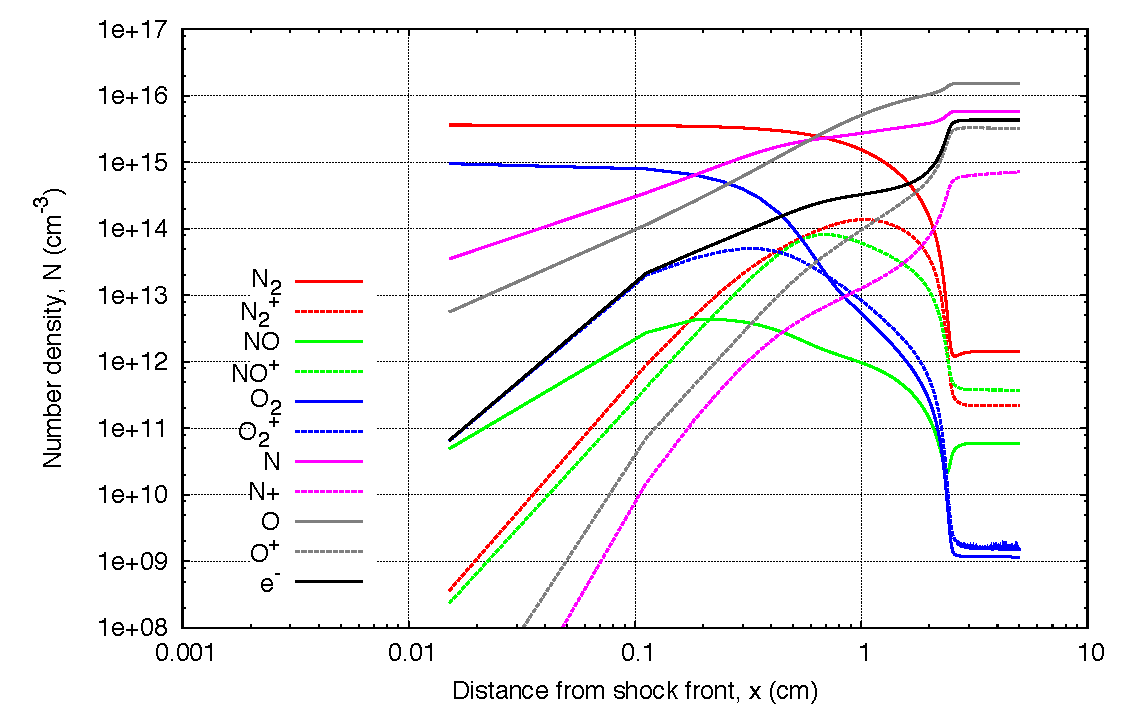
\includegraphics[width=0.9\linewidth]{figures/CR-modelling/FireII_1634s_number_densities.pdf} \label{fig:FireII_1634s_number_densities}} \\
 \subfloat[Radiative emission profile]{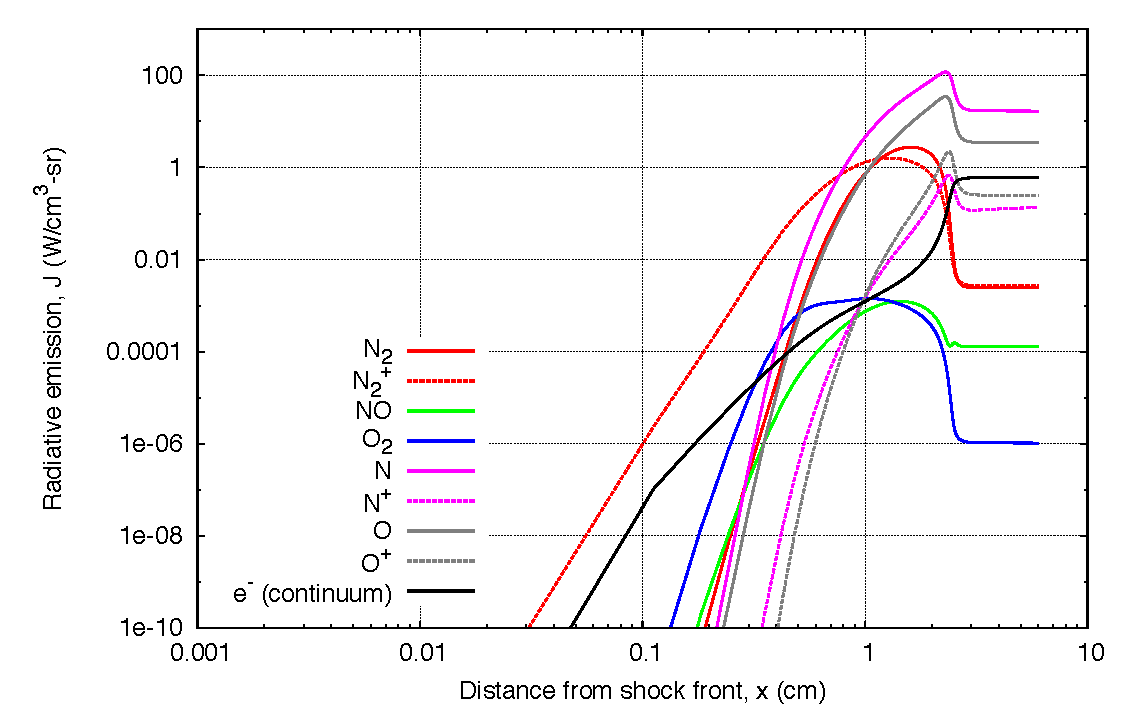
\includegraphics[width=0.9\linewidth]{figures/CR-modelling/FireII_1634s_emissions.pdf} \label{fig:FireII_1634s_emissions}}
 \caption{Post-shock species number density and radiative emission profiles along the stagnation streamline of the Fire II $t=1634$\,s condition ($p_\infty = 2$\,Pa, $T_\infty = 195$\,K, $u_\infty = 11,360$\,m/s).}
\end{figure}

Before deciding upon an appropriate collisional-radiative model for N$_2$--O$_2$ mixtures, it is instructive to consider a typical Earth re-entry shock layer.
Figures~\ref{fig:FireII_1634s_number_densities} and~\ref{fig:FireII_1634s_emissions} present post-shock species number density and radiative emission profiles respectively for the Fire II $t=1634$\,s condition.
For this analysis, the electronic states of the radiators are assumed to be populated by Boltzmann distributions.
Immediately behind the shock, O$_2$ rapidly dissociates and quickly forms a large population of O atoms, while N$_2$ dissociation proceeds at a slightly slower rate, leading to significant N$_2$ and N$_2^+$ radiation up to 2\,cm behind the shock.
The radiative emission of N$_2$ and N$_2^+$, however, is quickly exceeded by the lines of N and O as the heavily dissociated and partially ionised equilibrium state is approached.
As bound-bound transitions of NO, O$_2$, N$^+$ and O$^+$ only make minor contributions to the radiative emission, it is sufficient to consider the electronic levels of these species as being populated by Boltzmann distributions.
Conversely the radiative emission from N$_2$, N$_2^+$, N and O bound-bound transitions are significant, and the electronic levels of these species should be calculated via collision-radiative modelling.
Furthermore, as the free electron number density is almost the same order of magnitude as that of the heavy particles, reactions due to heavy particle impact can be omitted.


% - summarise model here in a table

\subsubsection{(a) Atomic species: N and O}

The collisional processes considered for the atomic species N and O are electron impact excitation and ionisation, and the radiative processes considered are bound-bound optically allowed transitions.
Table~\ref{tab:N-O-CR} summarises the implemented rate coefficients for each of these mechanisms.
Where more than one model are presented for a mechanism, they are listed in order of preference (\textit{e.g.} for the electron impact excitation of N, the rates of Frost \textit{et al.}~\cite{FAS+1998} are preferred with the remaining transitions described by the semi-empirical model of Gryzinski~\cite{Gryz59}).
%In the present work all the levels presented in Tables~\ref{tab:N-levels} and~\ref{tab:O-levels} for N and O respectively are considered as nonequilibrium levels.
\par

For the radiative transitions, the transition probabilities $A(i,j)$ for the nonequilibrium levels are calculated using Equation~\ref{eq:A_av} where the individual line transition probabilities are obtained from the NIST Atomic Species Database~\cite{NIST_ASD} (see Table~\ref{tab:atomic-lines}).
For the electron impact transitions, the rate coefficients $K_e(i,j)$ and $K_e(i,c)$ are either calculated using semi-empirical models or obtained directly from the literature in the form of curve-fits.

\par

Although all electron impact excitation and ionisation rates for N and O are able to be calculated by the previously-described semi-empirical models, the hydrogenic assumptions of these models are not appropriate for transition originating from the inner core of electronic levels~\cite{park_1990}.
Rates derived from experimental measurements of theoretical calculations are therefore preferred for transitions originating from the ground and low lying metastable states.
Fortunately, experimental measurements and quantum mechanical calculations of these transitions are much simpler and more readily available than for the high lying levels.

\par

\begin{table}[h]
 \center
 \caption{Summary of the collisional-radiative mechanisms implemented for N and O.}
 \label{tab:N-O-CR}
 \begin{tabular*}{1.0\textwidth}{cccc}
  \hline Species                         & Electronic levels & CR mechanisms                                & Models    \\
  \hline  
                  N                                & All & Electron impact excitation                & (a) Frost \textit{et al.}~\cite{FAS+1998} \\
                                                     &       &                                                               & (b) Gryzinski~\cite{Gryz59} \\
                                                     &       & Electron impact ionisation               & (a) Soon and Kunc~\cite{SK1990} \\
                                                     &       &                                                               & (b) Drawin (Reference~\cite{panesi_phd}) \\
                                                     &       & Radiative decay                                 & NIST Atomic Spectra Database~\cite{NIST_ASD} \\
                  O                                & All & Electron impact excitation                & (a) Zatsarinny and Tayal~\cite{ZT2003} \\
                                                     &       &                                                               & (b) Gryzinski~\cite{Gryz59} \\
                                                     &       & Electron impact ionisation               & (a) Soon and Kunc~\cite{SK1990} \\
                                                     &       &                                                               & (b) Drawin (Reference~\cite{panesi_phd}) \\
                                                     &       & Radiative decay                                 & NIST Atomic Spectra Database~\cite{NIST_ASD} \\                                   
  \hline
 \end{tabular*}
\end{table}

\subsubsection{(a) Electron impact excitation of N}

Frost \textit{et al.}~\cite{FAS+1998} performed R-matrix calculations for N and N$^+$ electron impact excitation transitions from the first 3 energy levels to all levels with principle quantum number $n$ less than 3.
Panesi~\cite{panesi_2008B} demonstrated improved agreement with the EAST shock tube data when implementing this model for N.
The rate coefficient is given as a function of the effective collision strength $\gamma_{i,j}$:

\begin{equation}
 K_e (i,j) = 2 \sqrt{\pi} \alpha c a_{0}^2 \sqrt{\frac{E_H}{kT_e}} \frac{\gamma_{i,j}(T_{e})}{g_i} \text{exp} \left ( - \frac{\Delta E_{i,j}}{kT_e} \right ),
\end{equation}

\noindent where $\alpha$ is the fine structure constant and the effective collision strength $\gamma_{i,j}$ has been curve fitted against the tabulated values provided by Frost in the range $0.5 \leq T_e \leq 12.0\text{\,eV}$.

\par

Bultel \textit{et al.}~\cite{BBB+2006} presented electron impact excitation and ionisation rates for the ground and metastable states of N and O.
These rates were presented as generalised Arrhenius curve-fits in the temperature range 2,000 $\leq T \leq$ 10,000\,K and were implemented in the collisional-radiative model of Panesi~\cite{panesi_phd}.
The excitation rates from the ground state of nitrogen are based on the $R$-matrix calculations of Berrington~\cite{BBR1975}.

\par

Figure~\ref{fig:K_EIE_N} compares the electron impact excitation rate coefficient for a selection of optically allowed and optically forbidden transitions of atomic nitrogen for which Frost \textit{et al.}~\cite{FAS+1998} present rate coefficients.
The indices of the initial $i$ and final $j$ electronic levels are given in the y-axis label in the form $K_e(i,j)$.
For the ground to first and second excited level transitions, Figures~\ref{fig:K_EIE_N_1_to_2} and~\ref{fig:K_EIE_N_1_to_3} respectively, the $R$-matrix based rates of Bultel and Frost are bounded by the semi-empirical Gryzinski and Drawin models.
The Bultel rates are up to an order of magnitude lower than the Frost rates for the $\Nlevone \Rightarrow \Nlevtwo$ optically forbidden transition.
For these transitions the theoretical calculations of Frost \textit{et al.}~\cite{FAS+1998} are preferred as they are more recent than those of Berrington~\cite{BBR1975}.

\begin{figure}[p]
 \centering
 \subfloat[$\Nlevone \Rightarrow \Nlevtwo$ (forbidden)]{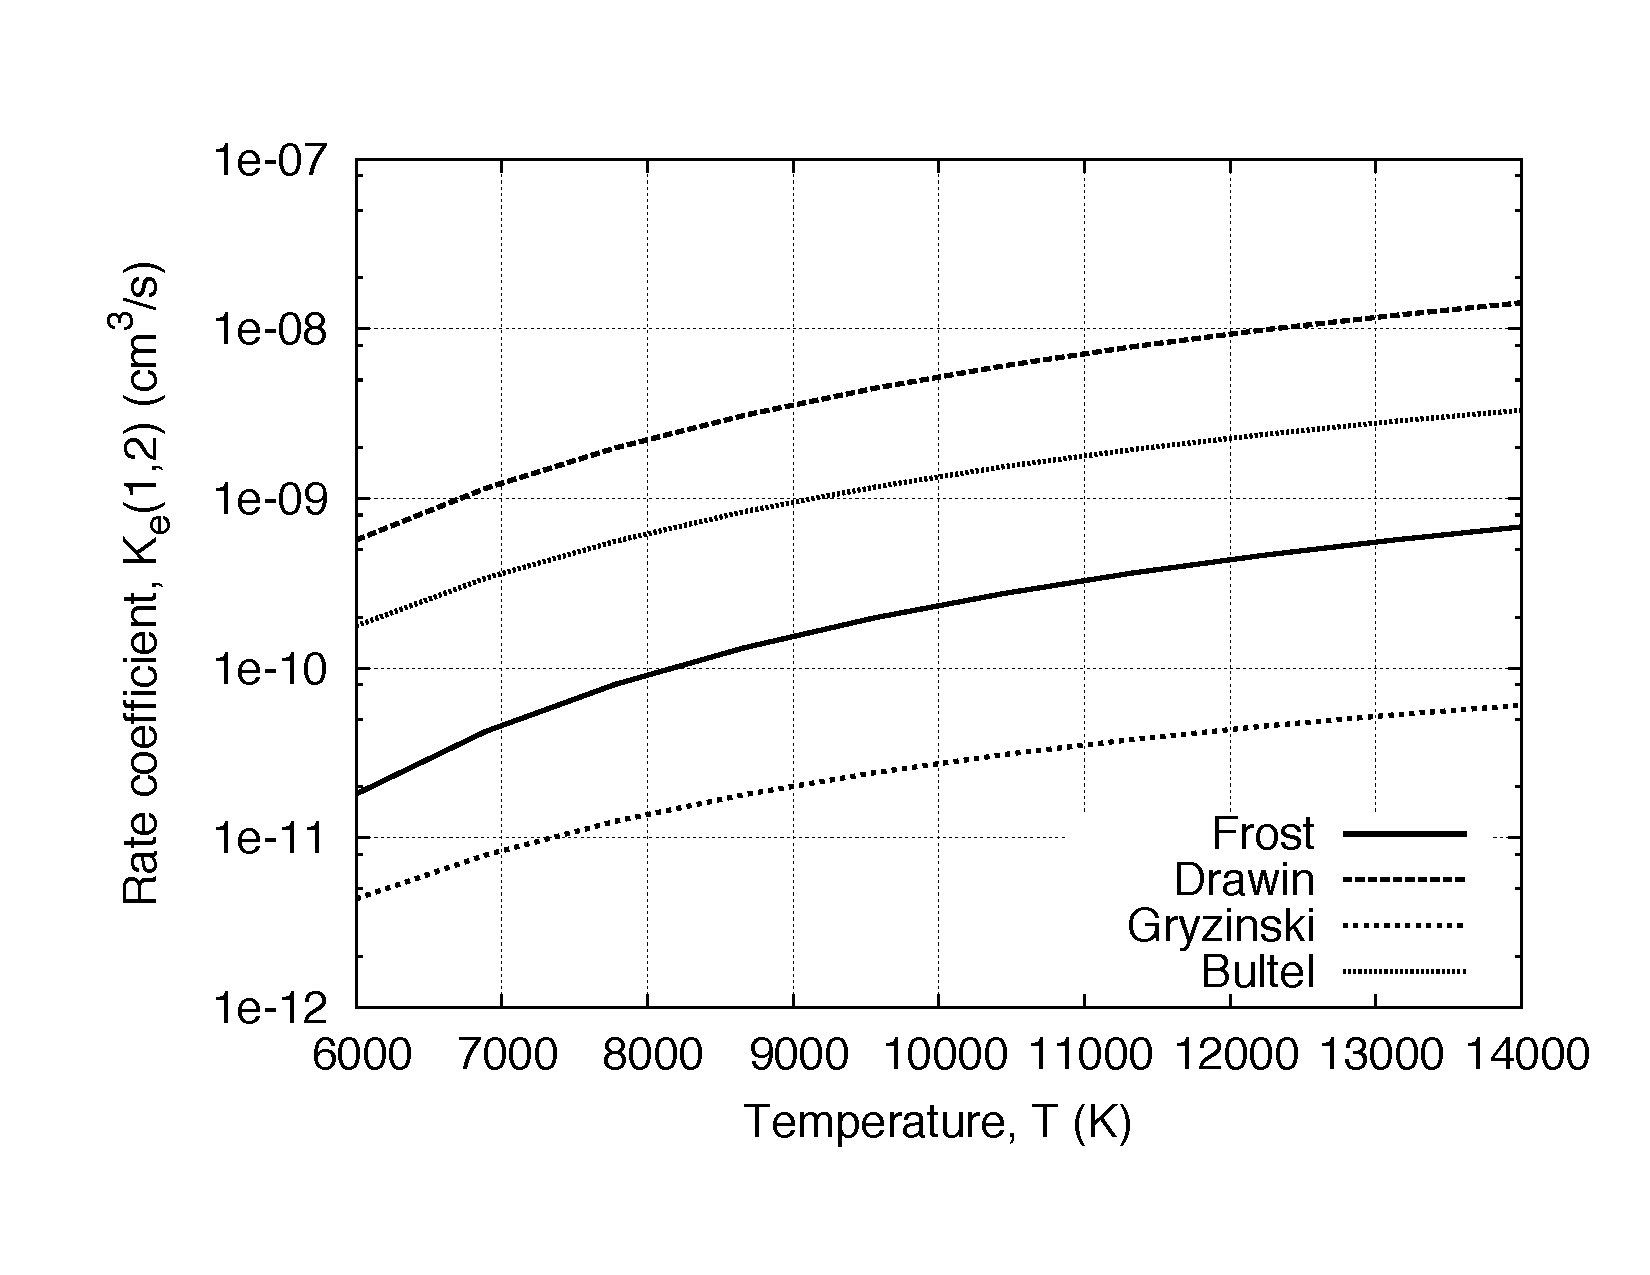
\includegraphics[width=0.48\linewidth]{figures/CR-modelling/K_EIE_N_1_to_2.pdf} \label{fig:K_EIE_N_1_to_2}}
 \subfloat[$\Nlevone \Rightarrow \Nlevthree$ (forbidden)]{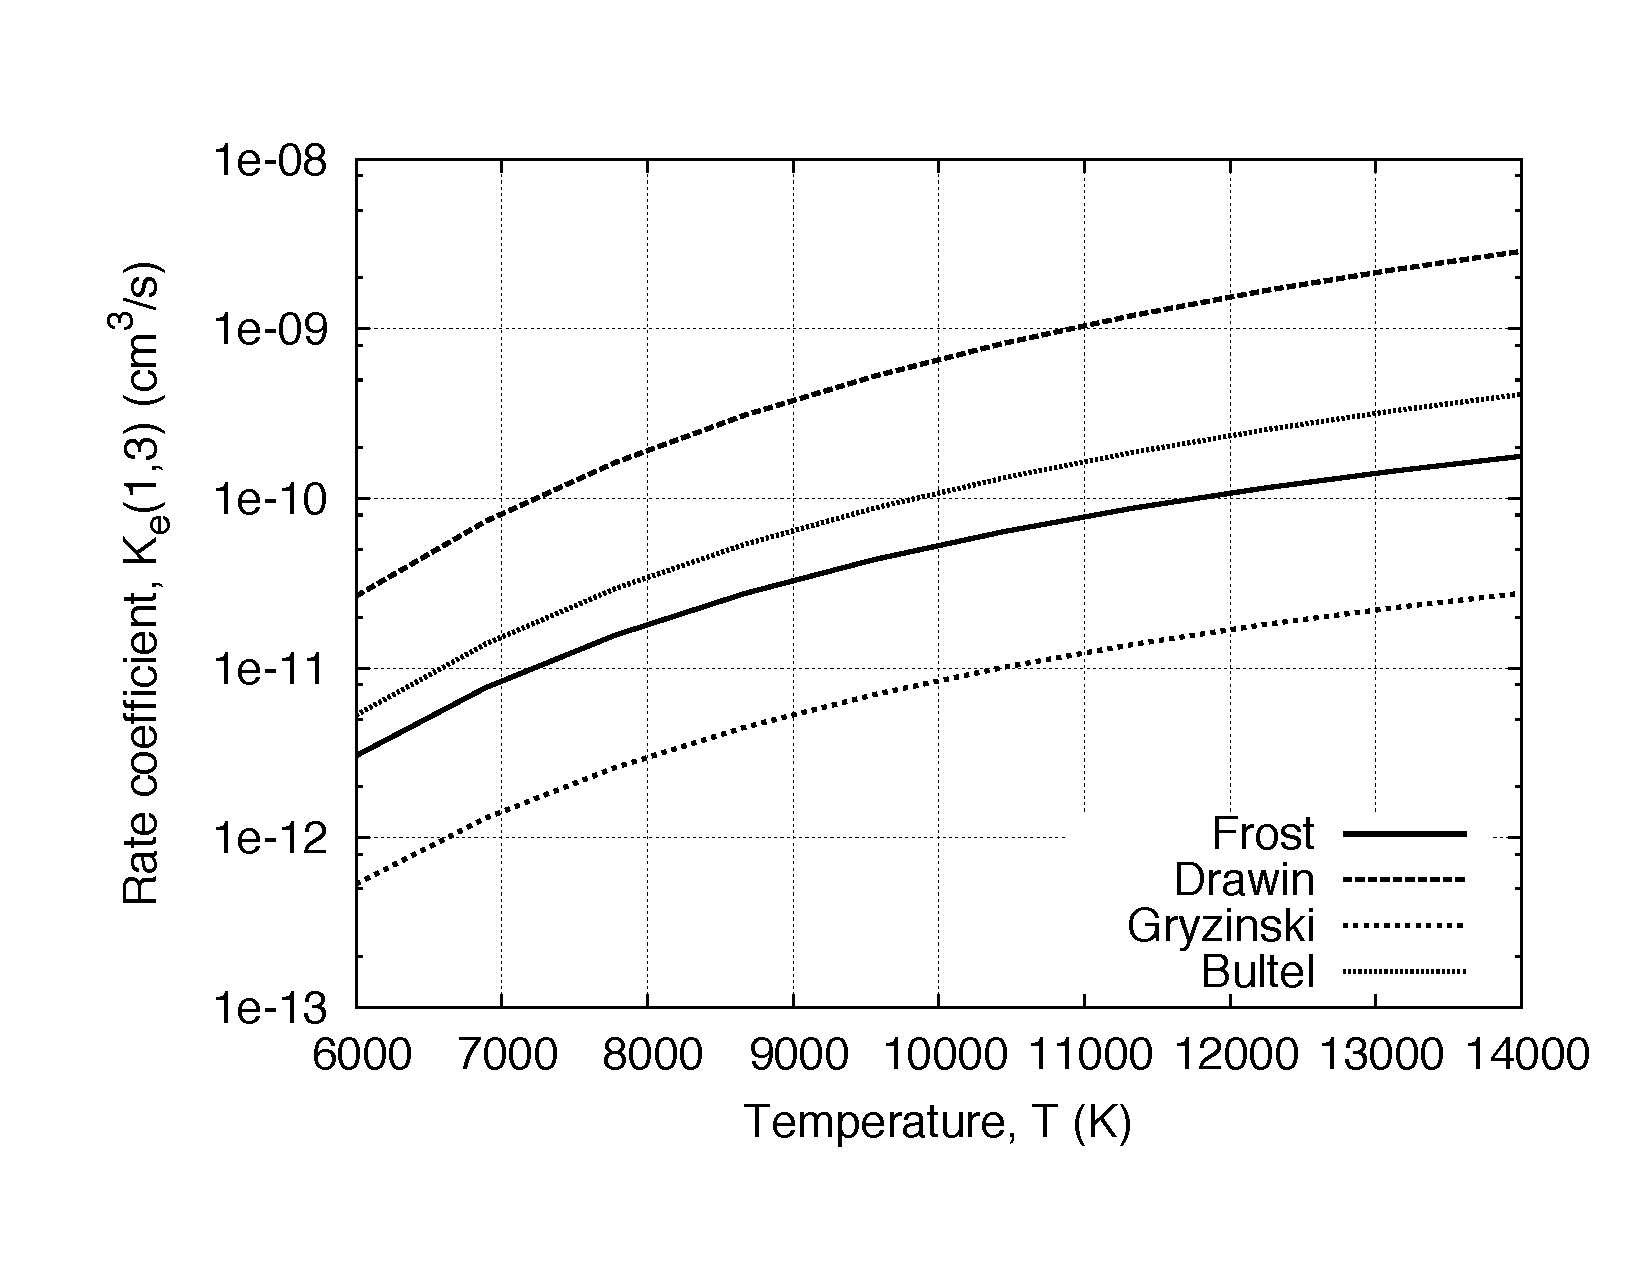
\includegraphics[width=0.48\linewidth]{figures/CR-modelling/K_EIE_N_1_to_3.pdf} \label{fig:K_EIE_N_1_to_3}} \\
 \subfloat[$\Nlevone \Rightarrow \Nlevfive$ (forbidden)]{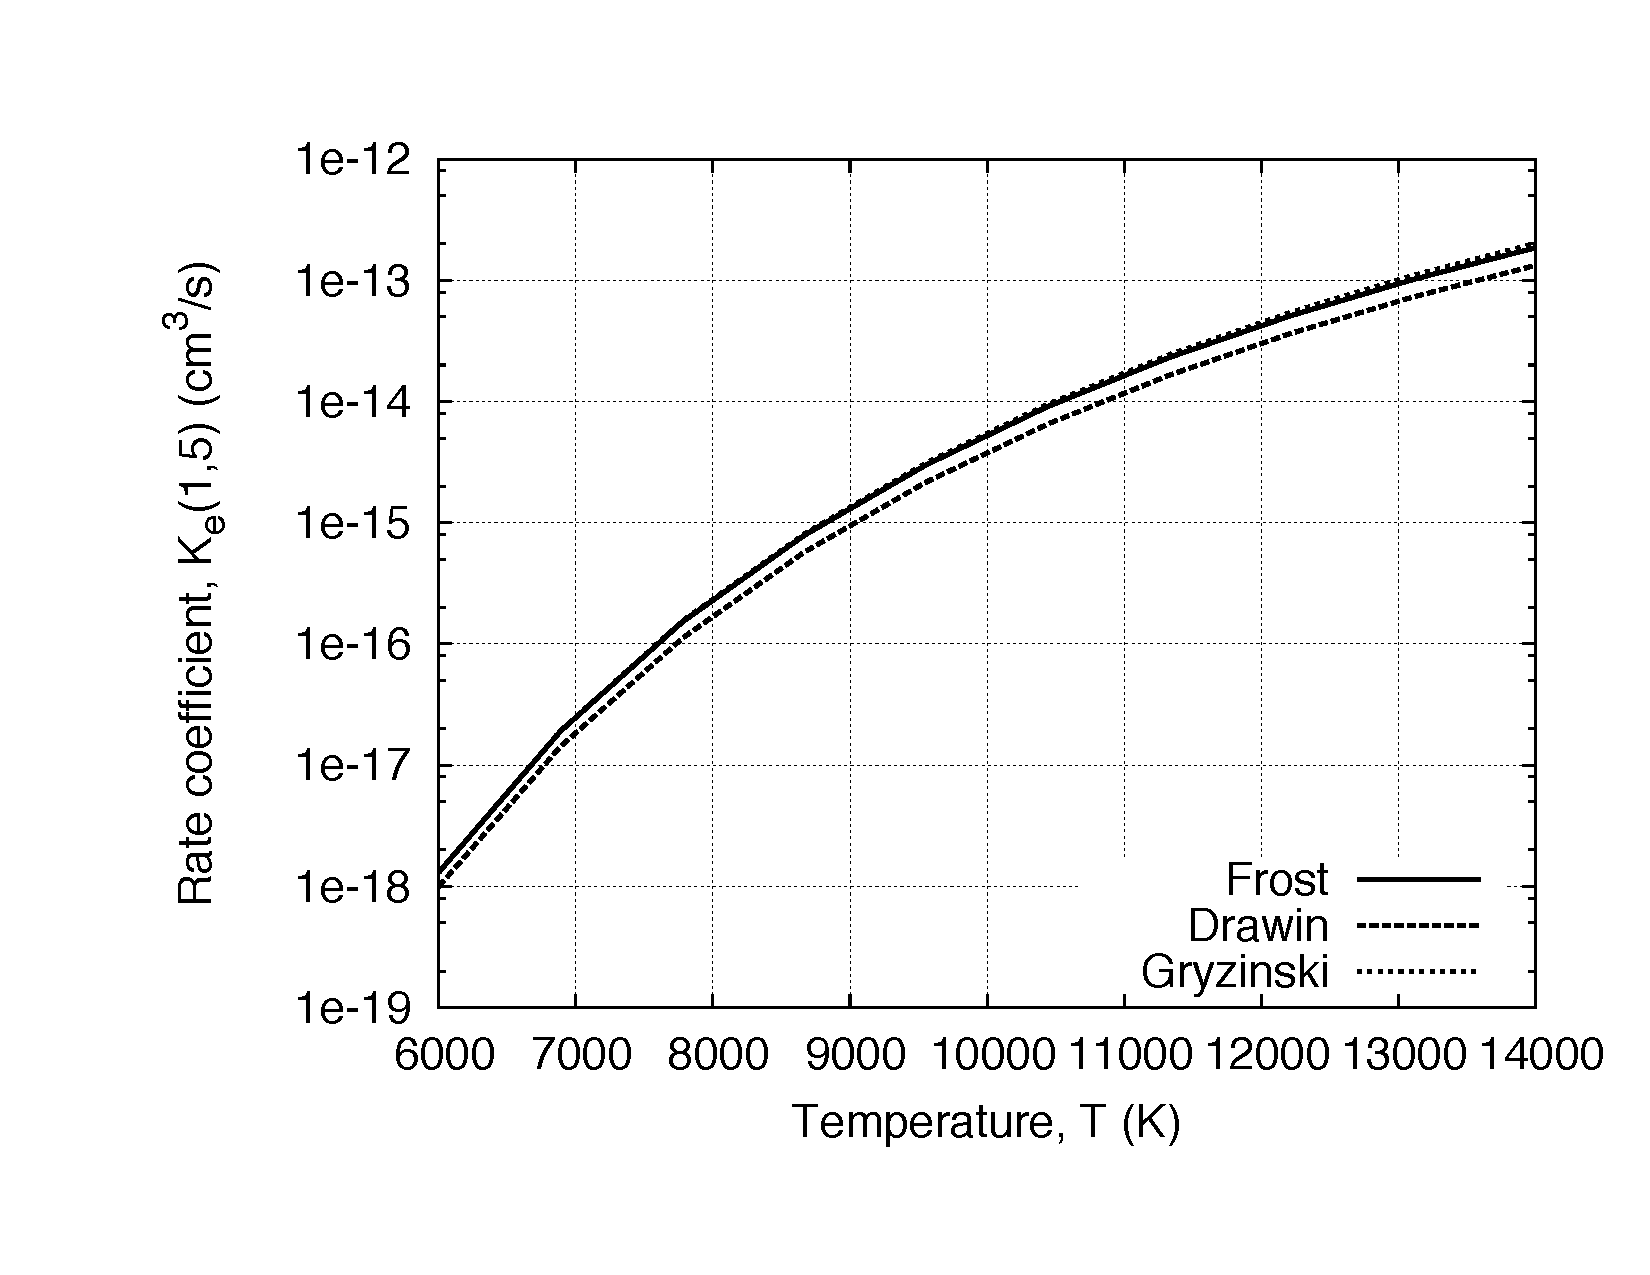
\includegraphics[width=0.48\linewidth]{figures/CR-modelling/K_EIE_N_1_to_5.pdf} \label{fig:K_EIE_N_1_to_5}}
 \subfloat[$\Nlevtwo \Rightarrow \Nlevfive$ (allowed)]{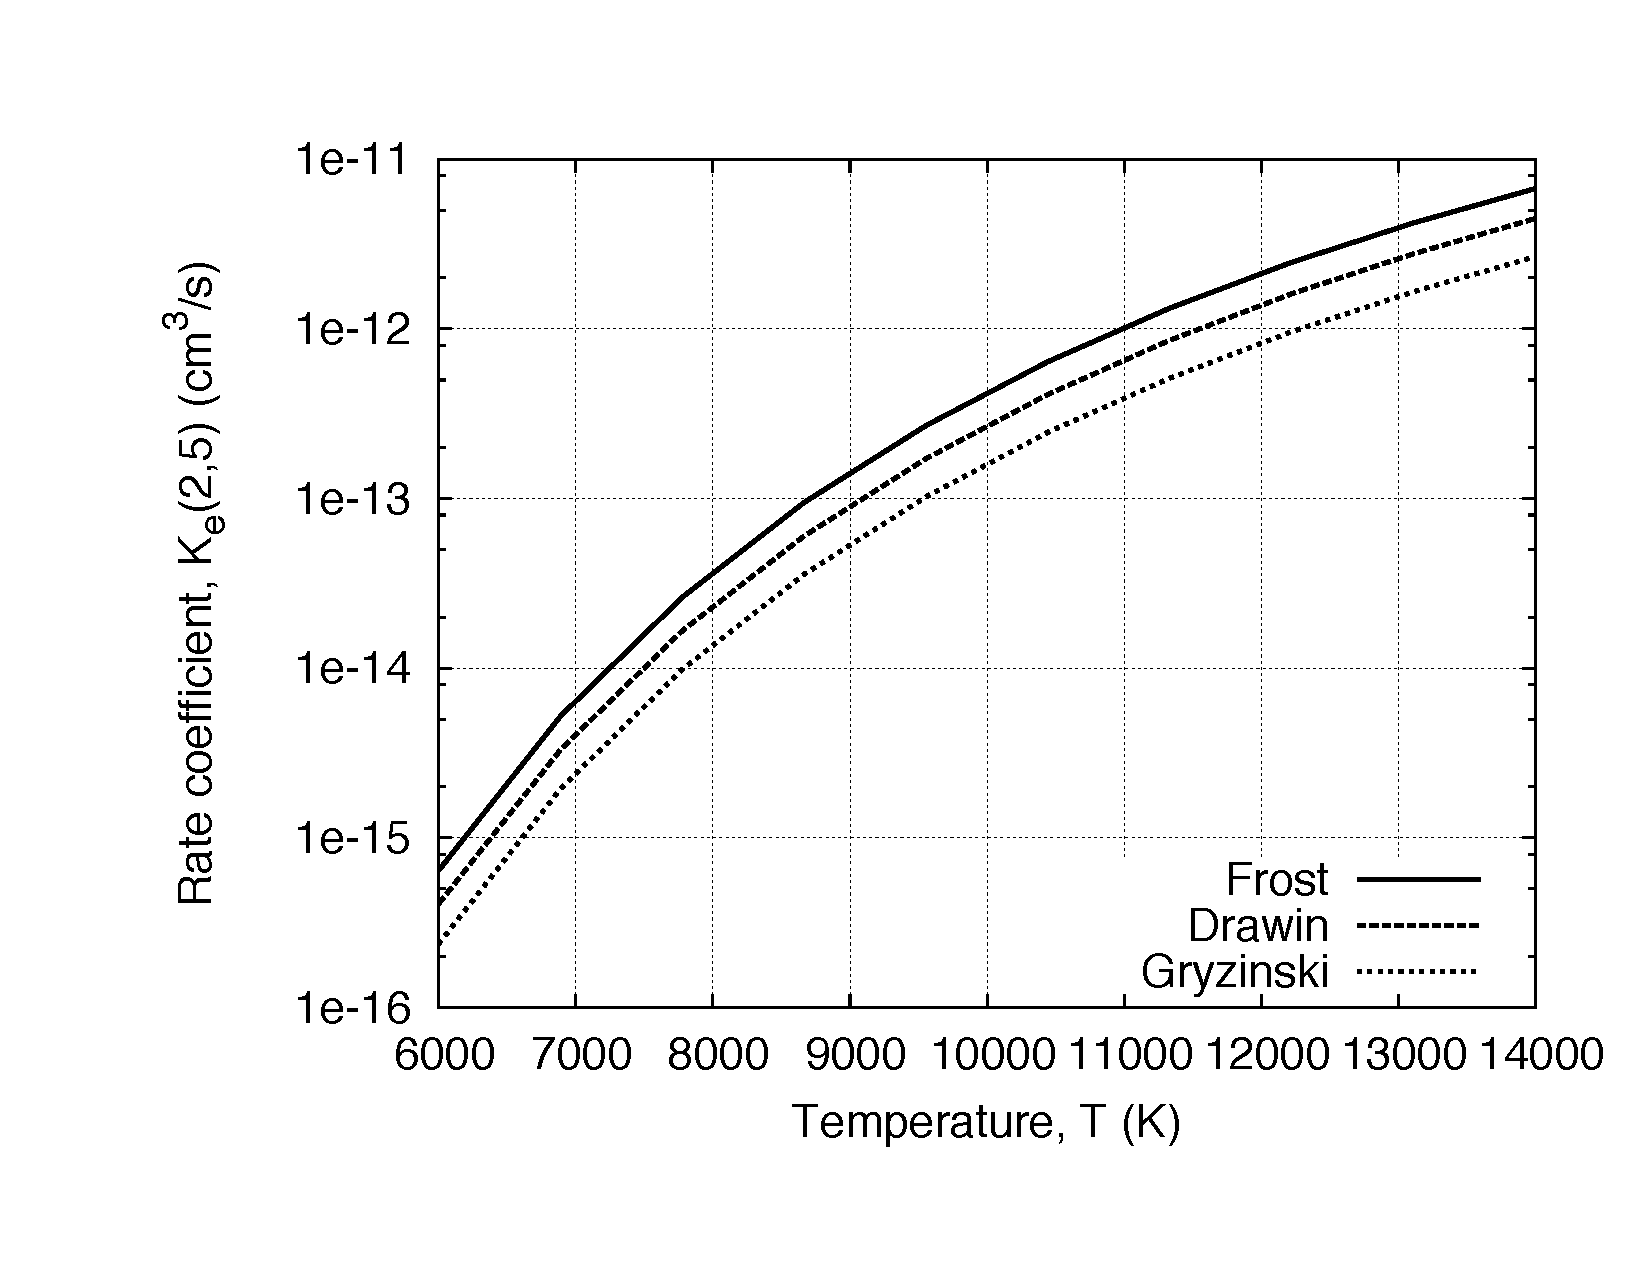
\includegraphics[width=0.48\linewidth]{figures/CR-modelling/K_EIE_N_2_to_5.pdf} \label{fig:K_EIE_N_2_to_5}} \\
  \subfloat[$\Nlevtwo \Rightarrow \Nlevthirteen$ (allowed)]{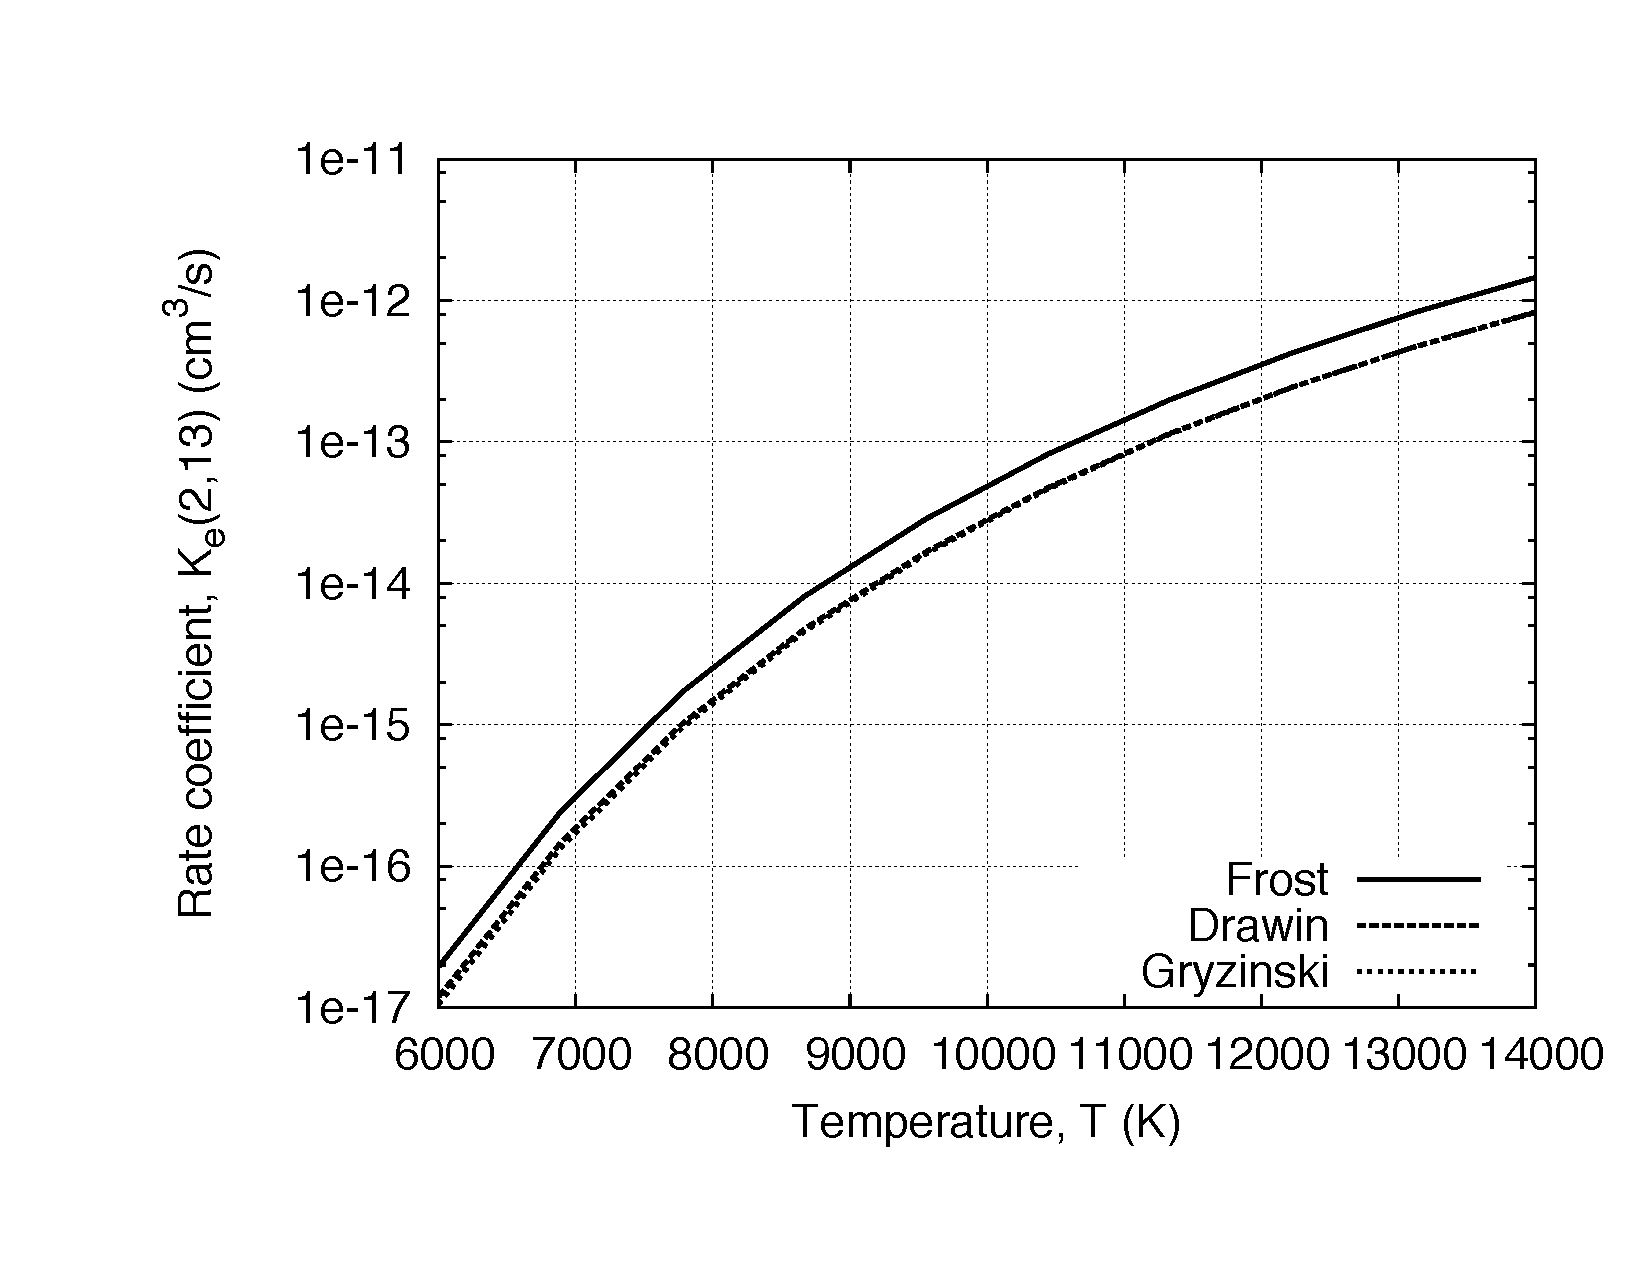
\includegraphics[width=0.48\linewidth]{figures/CR-modelling/K_EIE_N_2_to_13.pdf} \label{fig:K_EIE_N_2_to_13}}
 \subfloat[$\Nlevthree \Rightarrow \Nlevfifteen$ (allowed)]{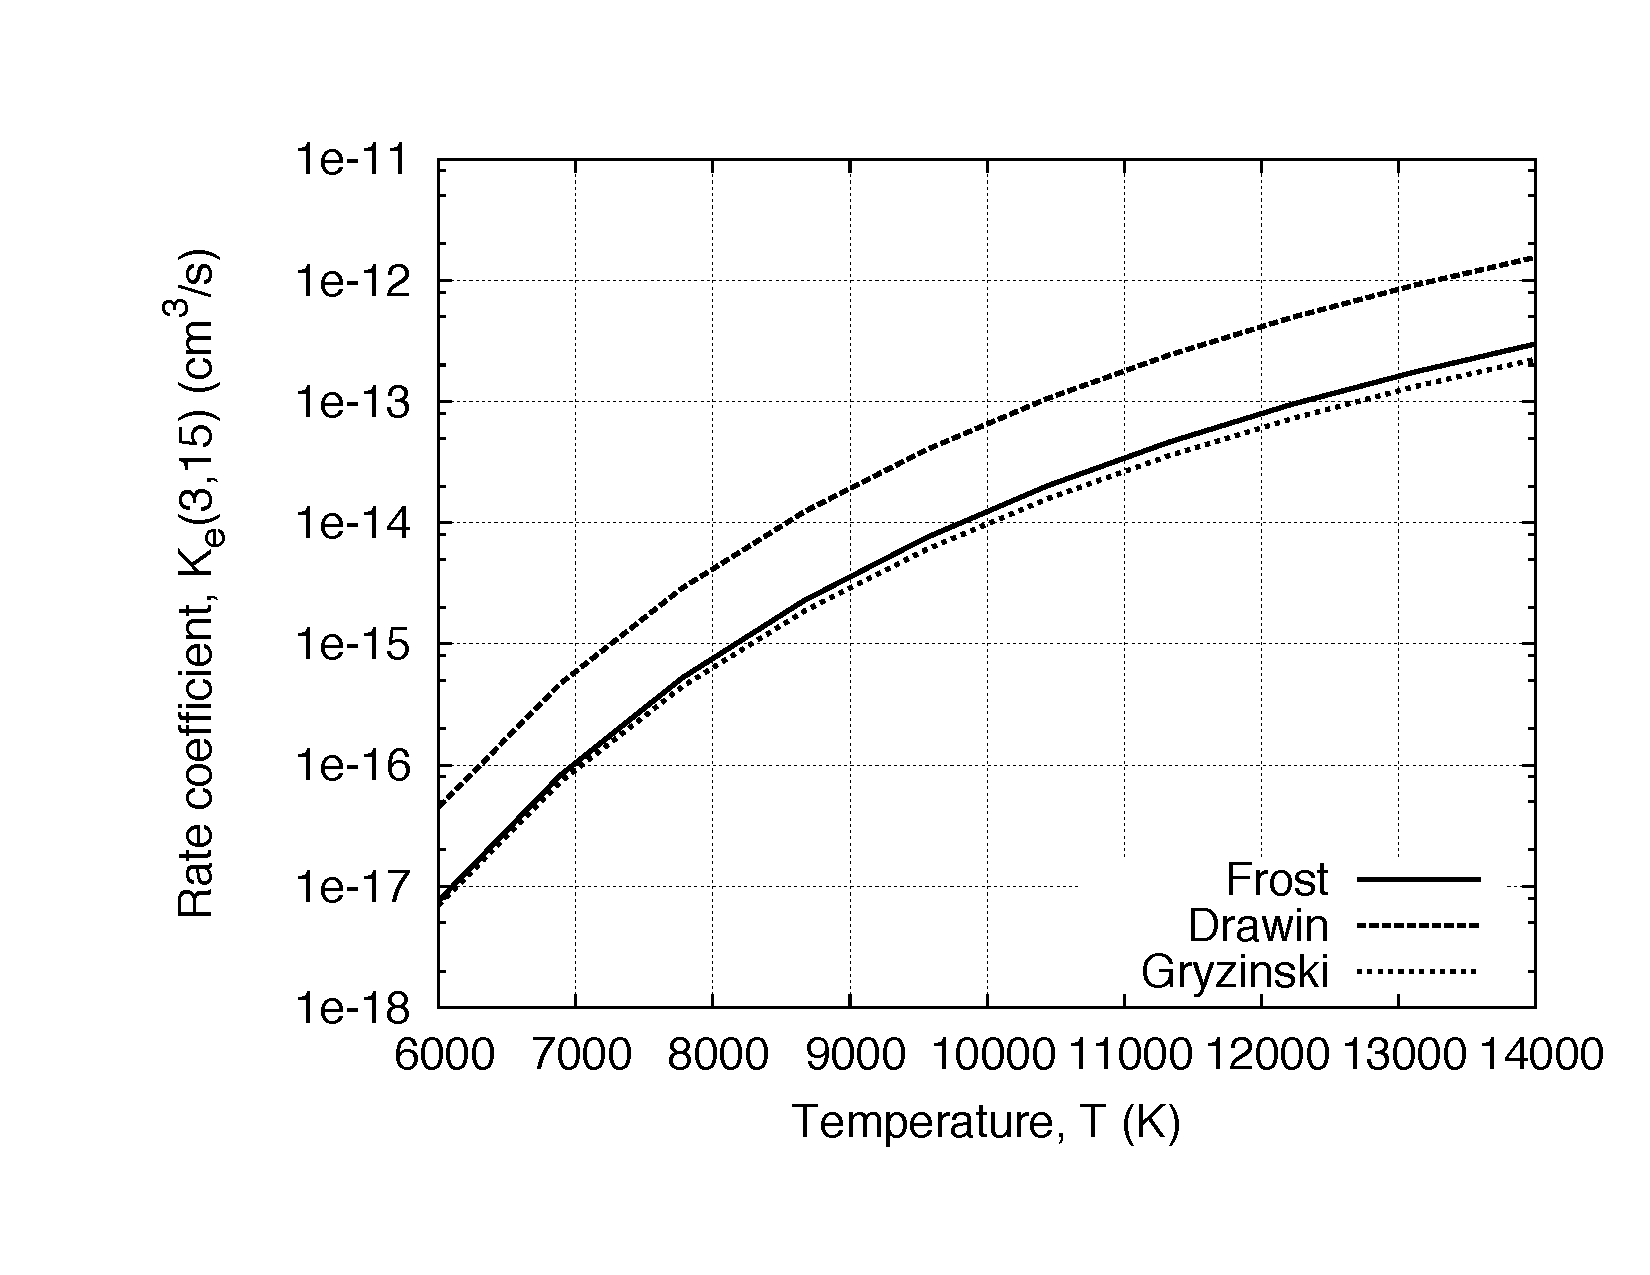
\includegraphics[width=0.48\linewidth]{figures/CR-modelling/K_EIE_N_3_to_15.pdf} \label{fig:K_EIE_N_3_to_15}} \\
 \caption{Comparison of  electron impact excitation rate coefficients for atomic nitrogen.}
 \label{fig:K_EIE_N}
\end{figure}

\begin{figure}[h]
 \centering
 \ContinuedFloat
 \subfloat[$\Nlevone \Rightarrow \Nlevtwenty$ (forbidden)]{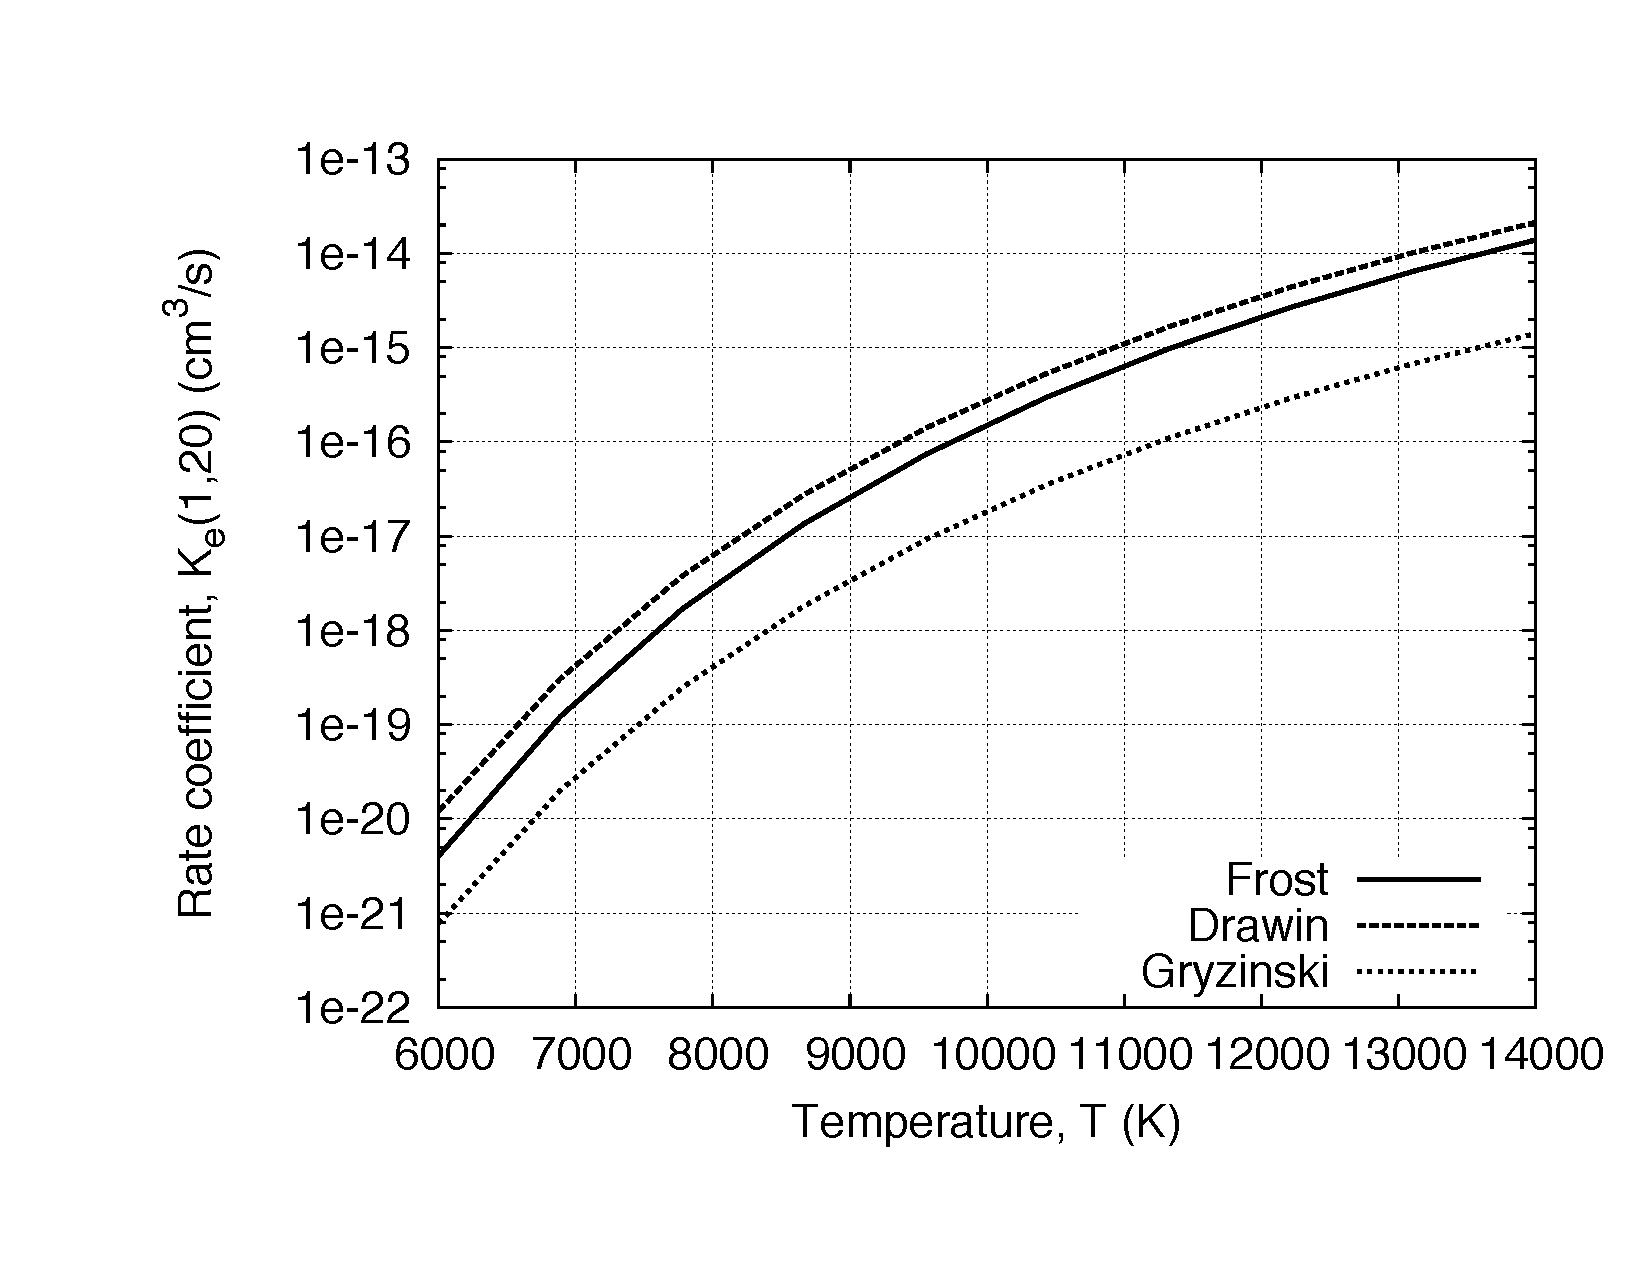
\includegraphics[width=0.48\linewidth]{figures/CR-modelling/K_EIE_N_1_to_20.pdf} \label{fig:K_EIE_N_1_to_20}}
 \subfloat[$\Nlevthree \Rightarrow \Nlevtwenty$ (forbidden)]{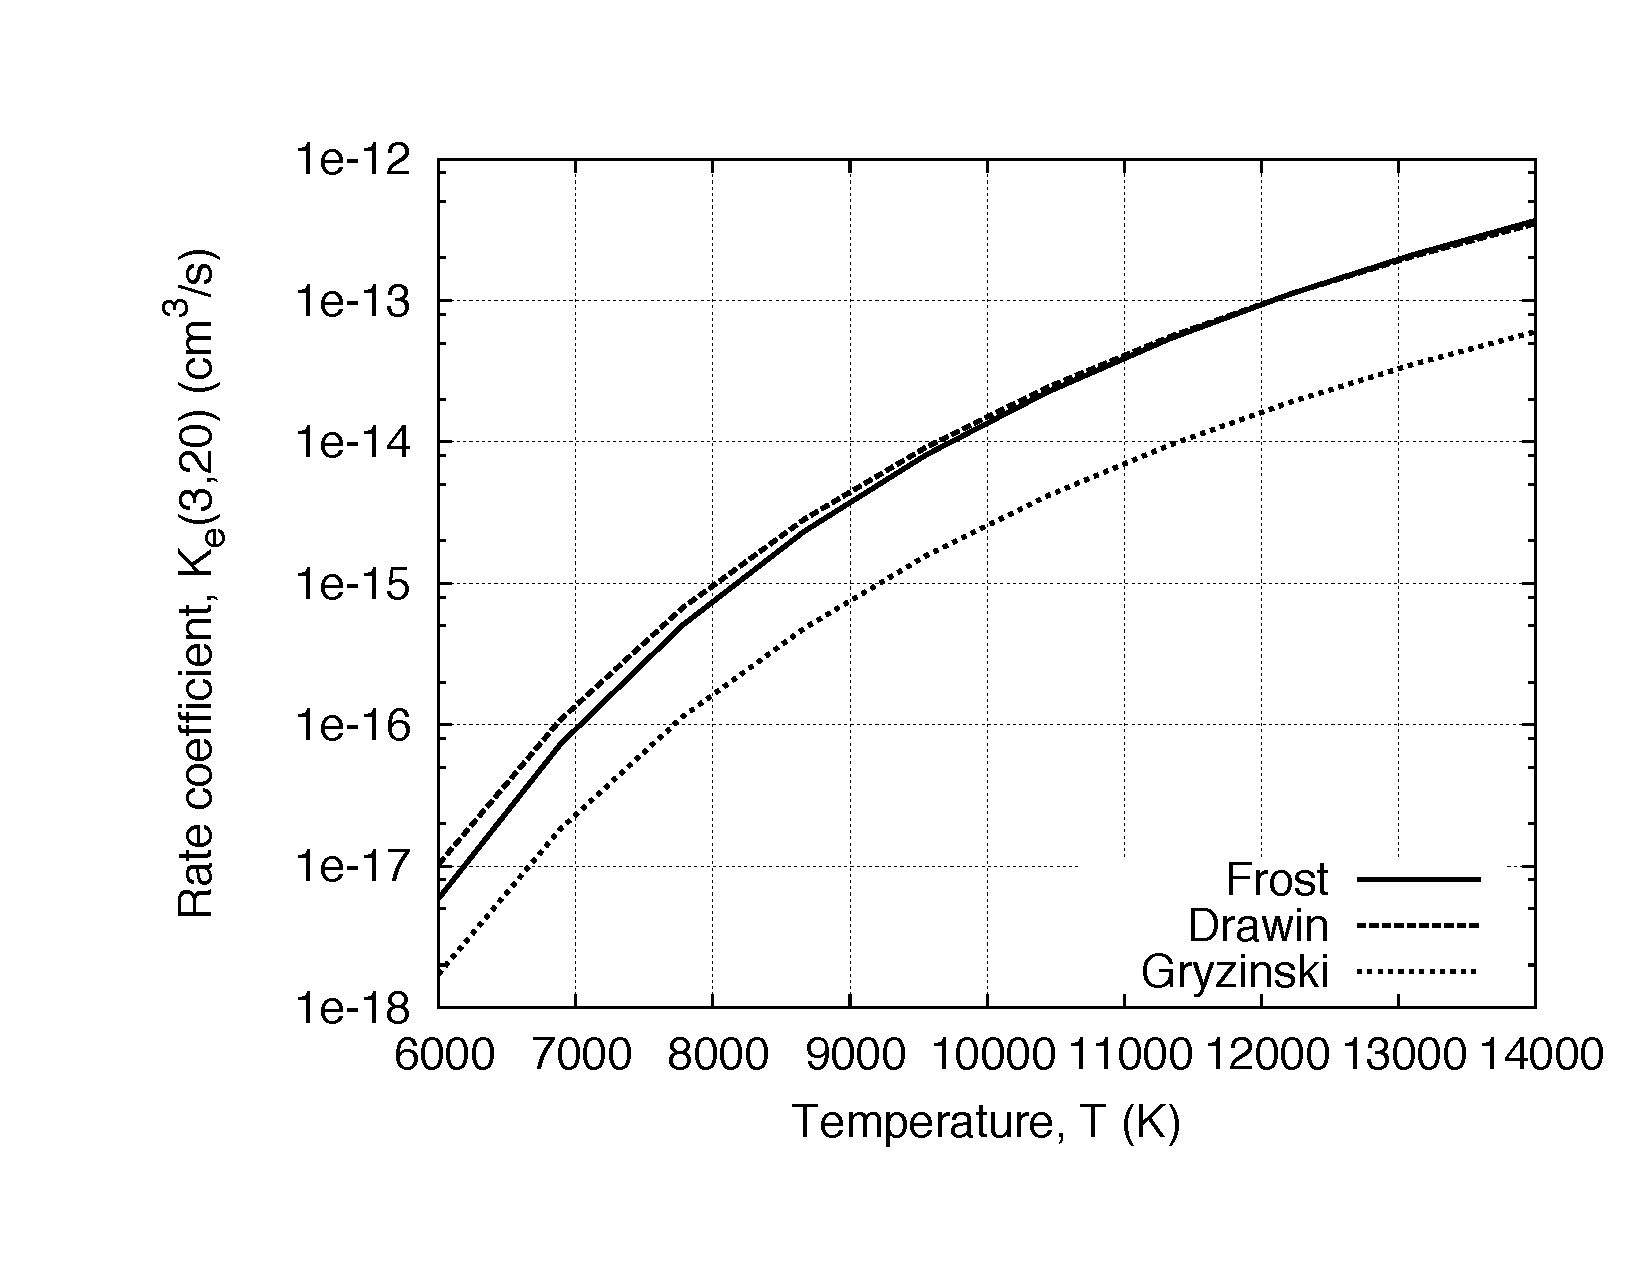
\includegraphics[width=0.48\linewidth]{figures/CR-modelling/K_EIE_N_3_to_20.pdf} \label{fig:K_EIE_N_3_to_20}}
 \caption{\textit{(Continued)} Comparison of  electron impact excitation rate coefficients for various transitions of N.}
 \label{fig:K_EIE_N}
\end{figure}

\par

The Frost, Drawin and Gryzinski models exhibit qualitative agreement for the remaining transitions shown, Figures~\ref{fig:K_EIE_N_1_to_5} to~\ref{fig:K_EIE_N_3_to_20}.
Quantitatively, it is encouraging to observe that the data of Frost is bounded by the Gryzinski and Drawin models for almost all transitions, although there is no trend as to which forms the upper or lower bound.
For the 1-5 and 3-15 transitions in Figures~\ref{fig:K_EIE_N_1_to_5} and~\ref{fig:K_EIE_N_3_to_15}, for example, the Gryzinski data shows exceptional agreement with the calculations of Frost.
In contrast, for the 1-20 and 3-20 transitions in Figures~\ref{fig:K_EIE_N_1_to_5} and~\ref{fig:K_EIE_N_3_to_20}, the Gryzinski model subtantially underestimates the data of Frost while the Drawin model shows good agreement.
Furthermore the semi-empirical models differ by up to two orders of magnitude for some transitions.
In the present work the theoretical calculations of Frost \textit{et al.}~\cite{FAS+1998} are preferred where available, with the remaining transitions described by the Gryzinski~\cite{Gryz59} model.
The decision to implement the Gryzinski model in preference to the Drawin model is based on the findings of Panesi~\cite{panesi_2008B,panesi_phd}, where the Gryzinski model gave improved agreement with the air shock tube spectroscopy experiments performed in the EAST facility.

\subsubsection{(b) Electron impact ionisation of N}

Johnston~\cite{JohnPhd} implemented the ionisation rate coefficients proposed by Kunc and Soon~\cite{KS1989} for the ground and first two excited levels of atomic nitrogen.
The rate coefficients are calculated as:

\begin{equation}
 K_e(i,c) = 1.0 \times 10^{-8} \left [ \frac{I_H}{I - E_i} \right ] \frac{Q_i}{2 l_i + 1} \text{exp} \left ( - \beta \right ) G_i \left ( \beta \right ) \label{eq:K_EII_Soon_Kunc_a}
\end{equation}

\noindent where,

\begin{equation}
 G_i ( \beta ) = \sqrt{\frac{\beta}{\beta+1}} \frac{A}{\beta + \chi} \text{ , }
\end{equation}

\noindent and, 

\begin{equation}
 \beta = \frac{I - E_i}{kT_e} \text{ . } \label{eq:K_EII_Soon_Kunc_c}
\end{equation}

\noindent The parameter $I_H$ is the ionisation energy of the hydrogen energy (Rydberg energy), $l_i$ is the angular momentum quantum number of the level $i$, $A$ and $\chi$ are fitting constants for the species and $G_i$ is level dependent angular factor.
For atomic nitrogen $A$ is equal to 27.71, $\chi$ is equal to 5.58 and $Q_i$ is equal to 3 for the ground state and $3/2$ for the first and second excited states.
This expression is a curve-fit based on the rate coefficient derived from experimentally measured electron impact ionisation cross sections for the ground state of N.

\par

Panesi~\cite{panesi_phd} implemented the ionisation rate coefficients presented by Bultel \textit{et al.}~\cite{BBB+2006}, which were obtained from the compilation of Tawara and Kato~\cite{TK1999} and the combined binary-encounter Bethe (BEB) and scaled plane-wave Born (PWB) calculations of Kim and Desclaux~\cite{KD2002}.
The rates for the ground and first two excited states of N were presented as generalised Arrhenius curve-fits in the temperature range 2,000 $\leq T_e \leq$ 10,000\,K.

\par

Figure~\ref{fig:K_EII_N} compares the electron impact ionisation rate coefficient for various transitions of N.
The experimentally-fitted Kunc and Soon rates and the theoretically-fitted Bultel rates are in good agreement for the ground and metastable states, Figures~\ref{fig:K_EII_N_1} to~\ref{fig:K_EII_N_3}.
%As was observed for the electron impact excitation rates, the Bultel generalised Arrhenius expressions substantially underestimates the rates of all other models --- by as much as six orders of magnitude for ionisation of the metastable states, Figures~\ref{fig:K_EII_N_2} and~\ref{fig:K_EII_N_3}.
%It is unclear how the Bultel rates are able to be valid in the quoted 2,000 $\leq T_e \leq$ 10,000\,K temperature range when the minimum electron temperature considered in the calculations of Kim and Desclaux~\cite{KD2002} is 12\,eV ($\approx$ 140,000\,K).
The Drawin models implemented by Johnston~\cite{JohnPhd} and Panesi~\cite{panesi_phd} bound the Kunc and Soon rates and Bultel rates, with Panesi's implementation being in closer agreement.
Although the difference between the two Drawin models decreases as ionisation from higher levels and low electron temperatures is considered (see Figure~\ref{fig:K_EII_N_13}), Johnston's implementation is between approximately 2 and 100 times smaller for all levels.
Therefore in the present work the experimentally-fitted electron impact ionisation coefficients of Soon and Kunc~\cite{SK1990} are preferred for the first three levels, while the Drawin model implemented by Panesi~\cite{JohnPhd} is used for the remaining levels.

\begin{figure}[th]
 \centering
 \subfloat[$\text{N } \Nlevone \Rightarrow \text{N}^+$]{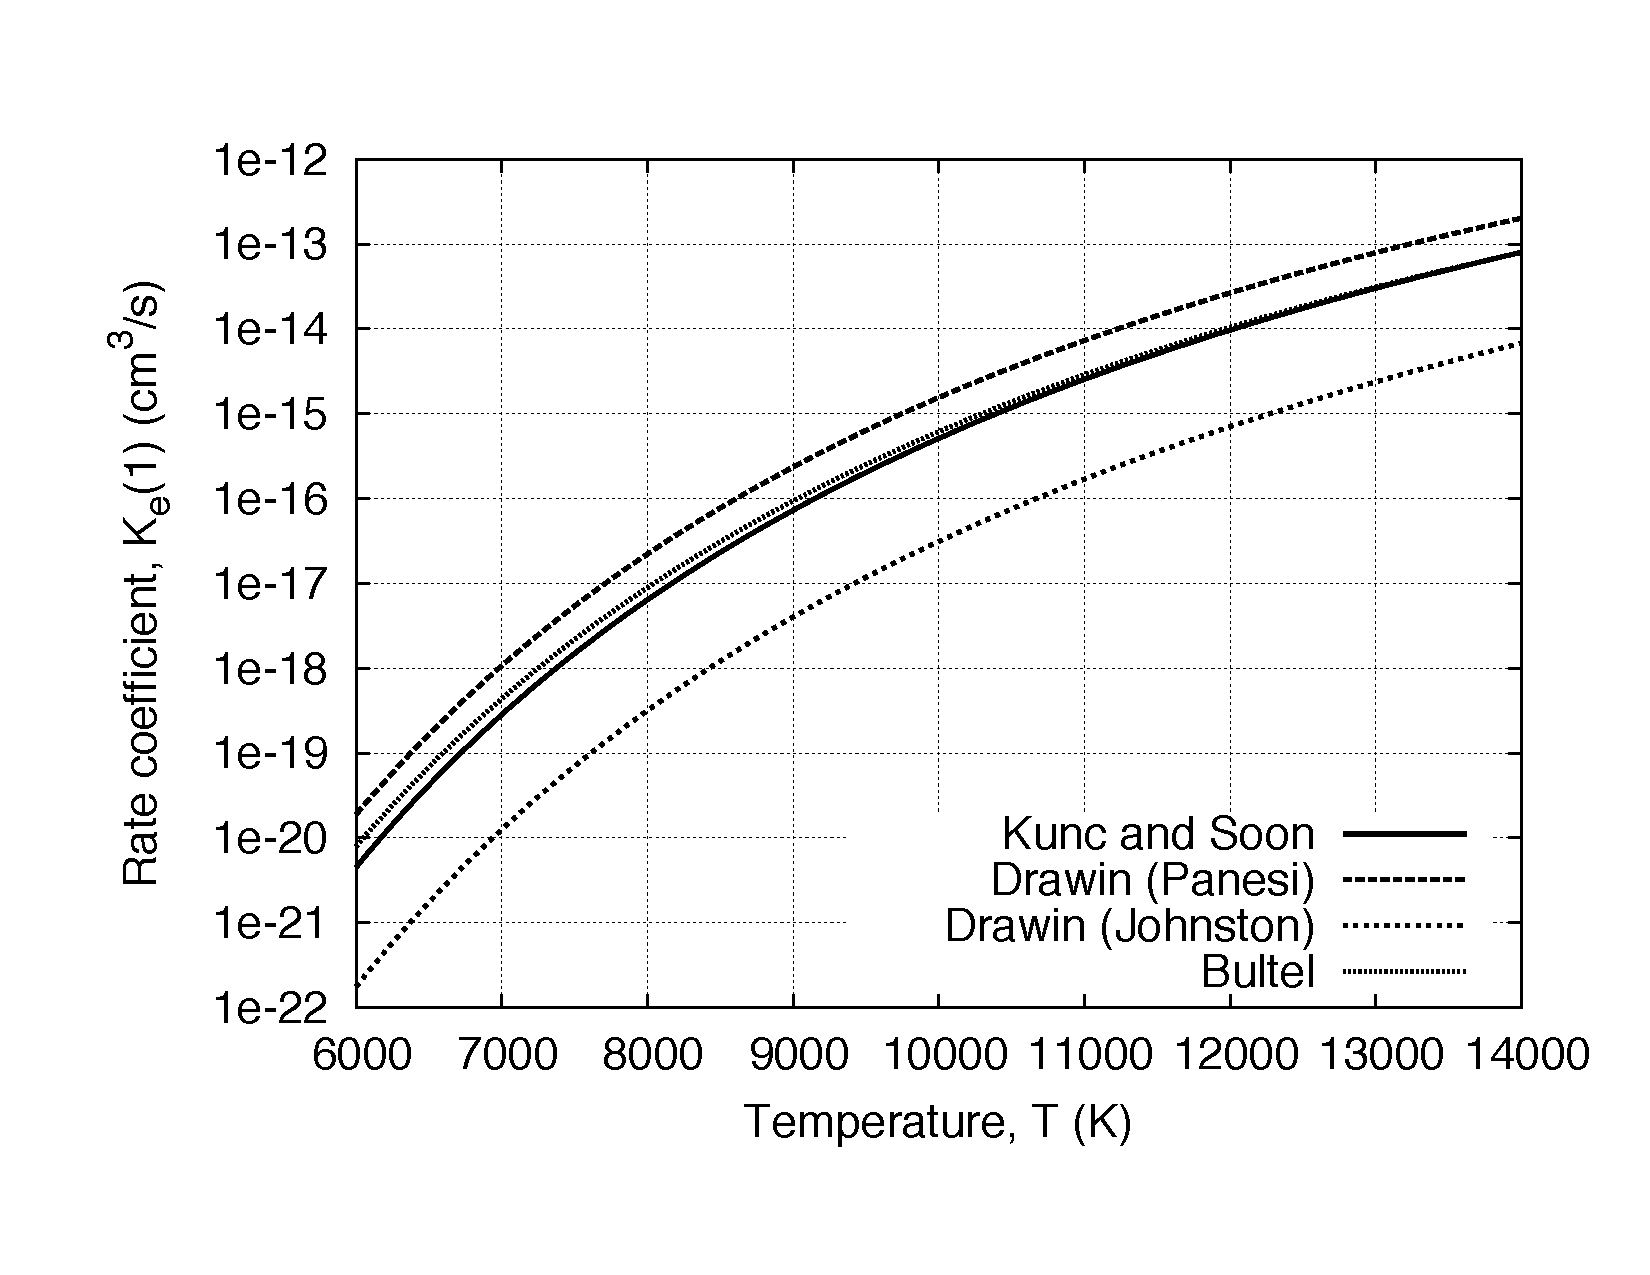
\includegraphics[width=0.48\linewidth]{figures/CR-modelling/K_EII_N_1.pdf} \label{fig:K_EII_N_1}}
 \subfloat[$\text{N } \Nlevtwo \Rightarrow \text{N}^+$]{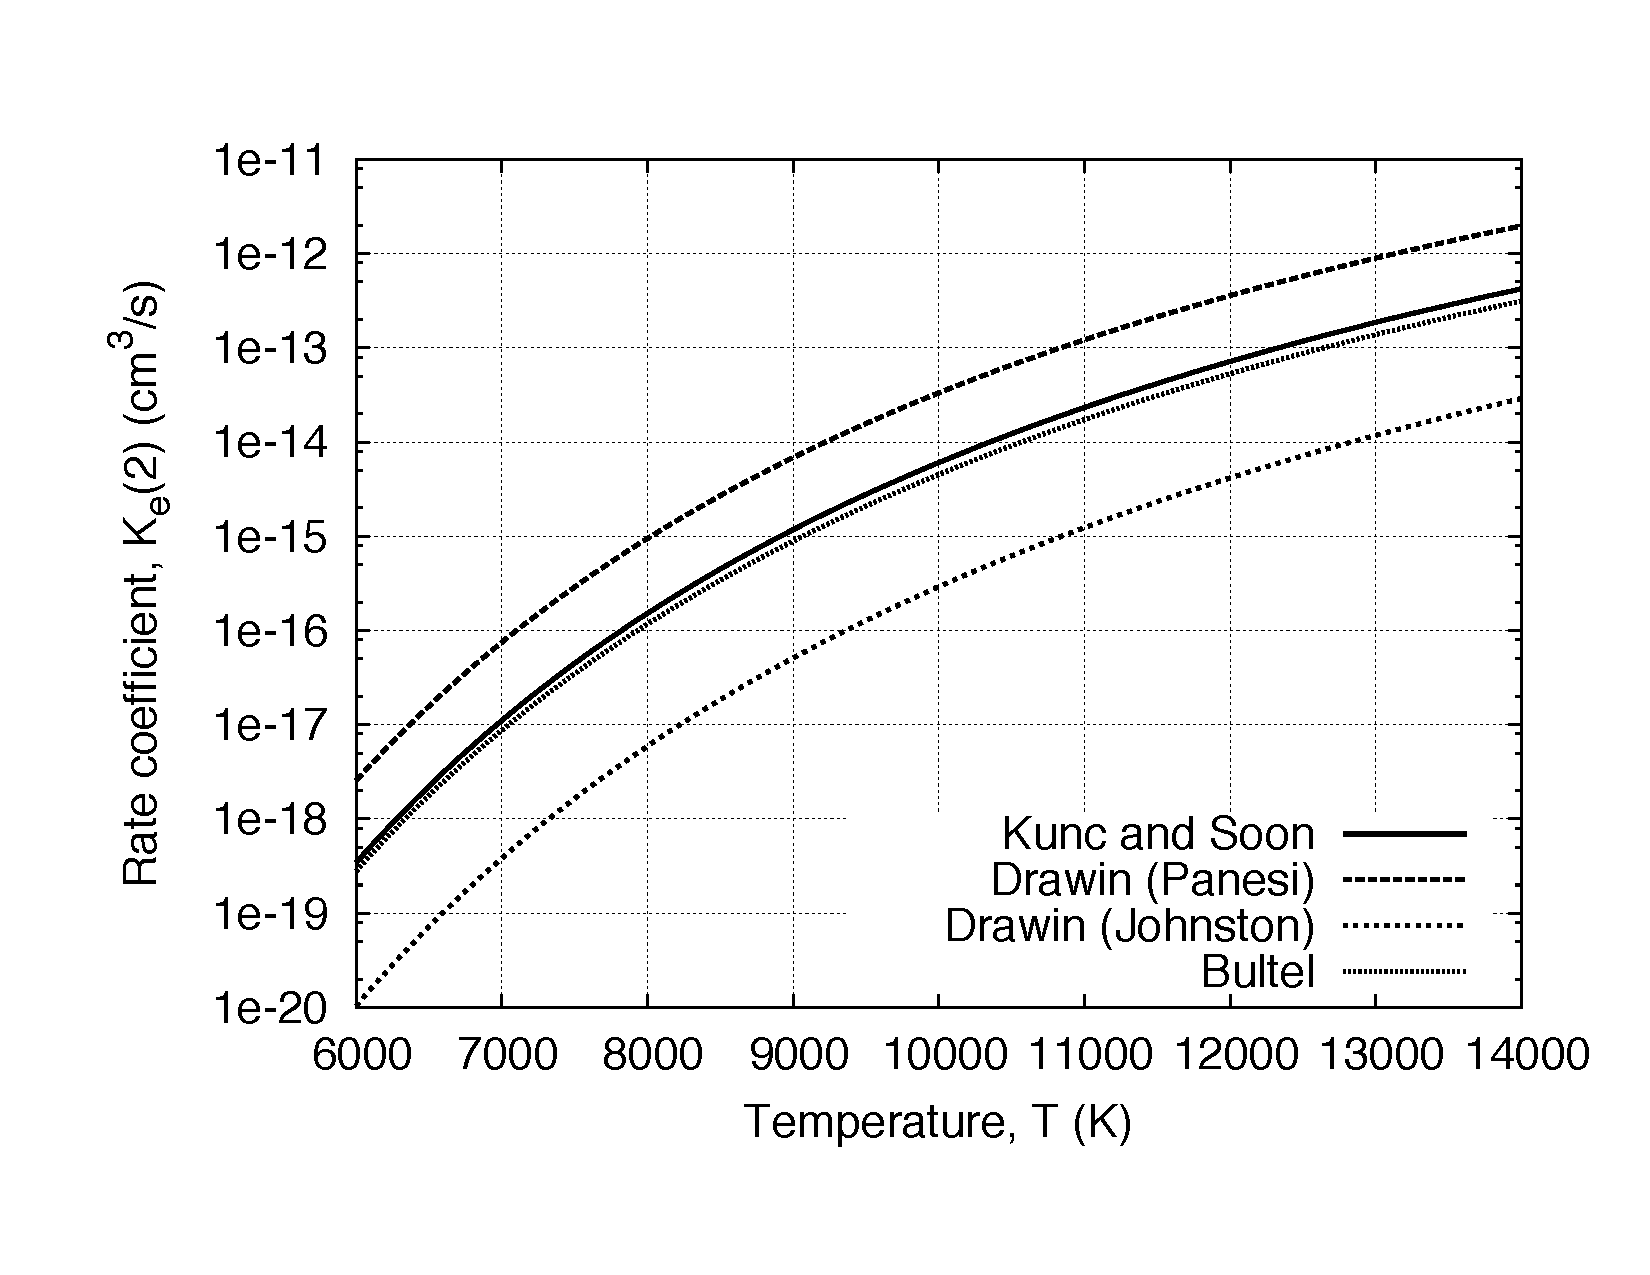
\includegraphics[width=0.48\linewidth]{figures/CR-modelling/K_EII_N_2.pdf} \label{fig:K_EII_N_2}} \\
 \subfloat[$\text{N } \Nlevthree \Rightarrow \text{N}^+$]{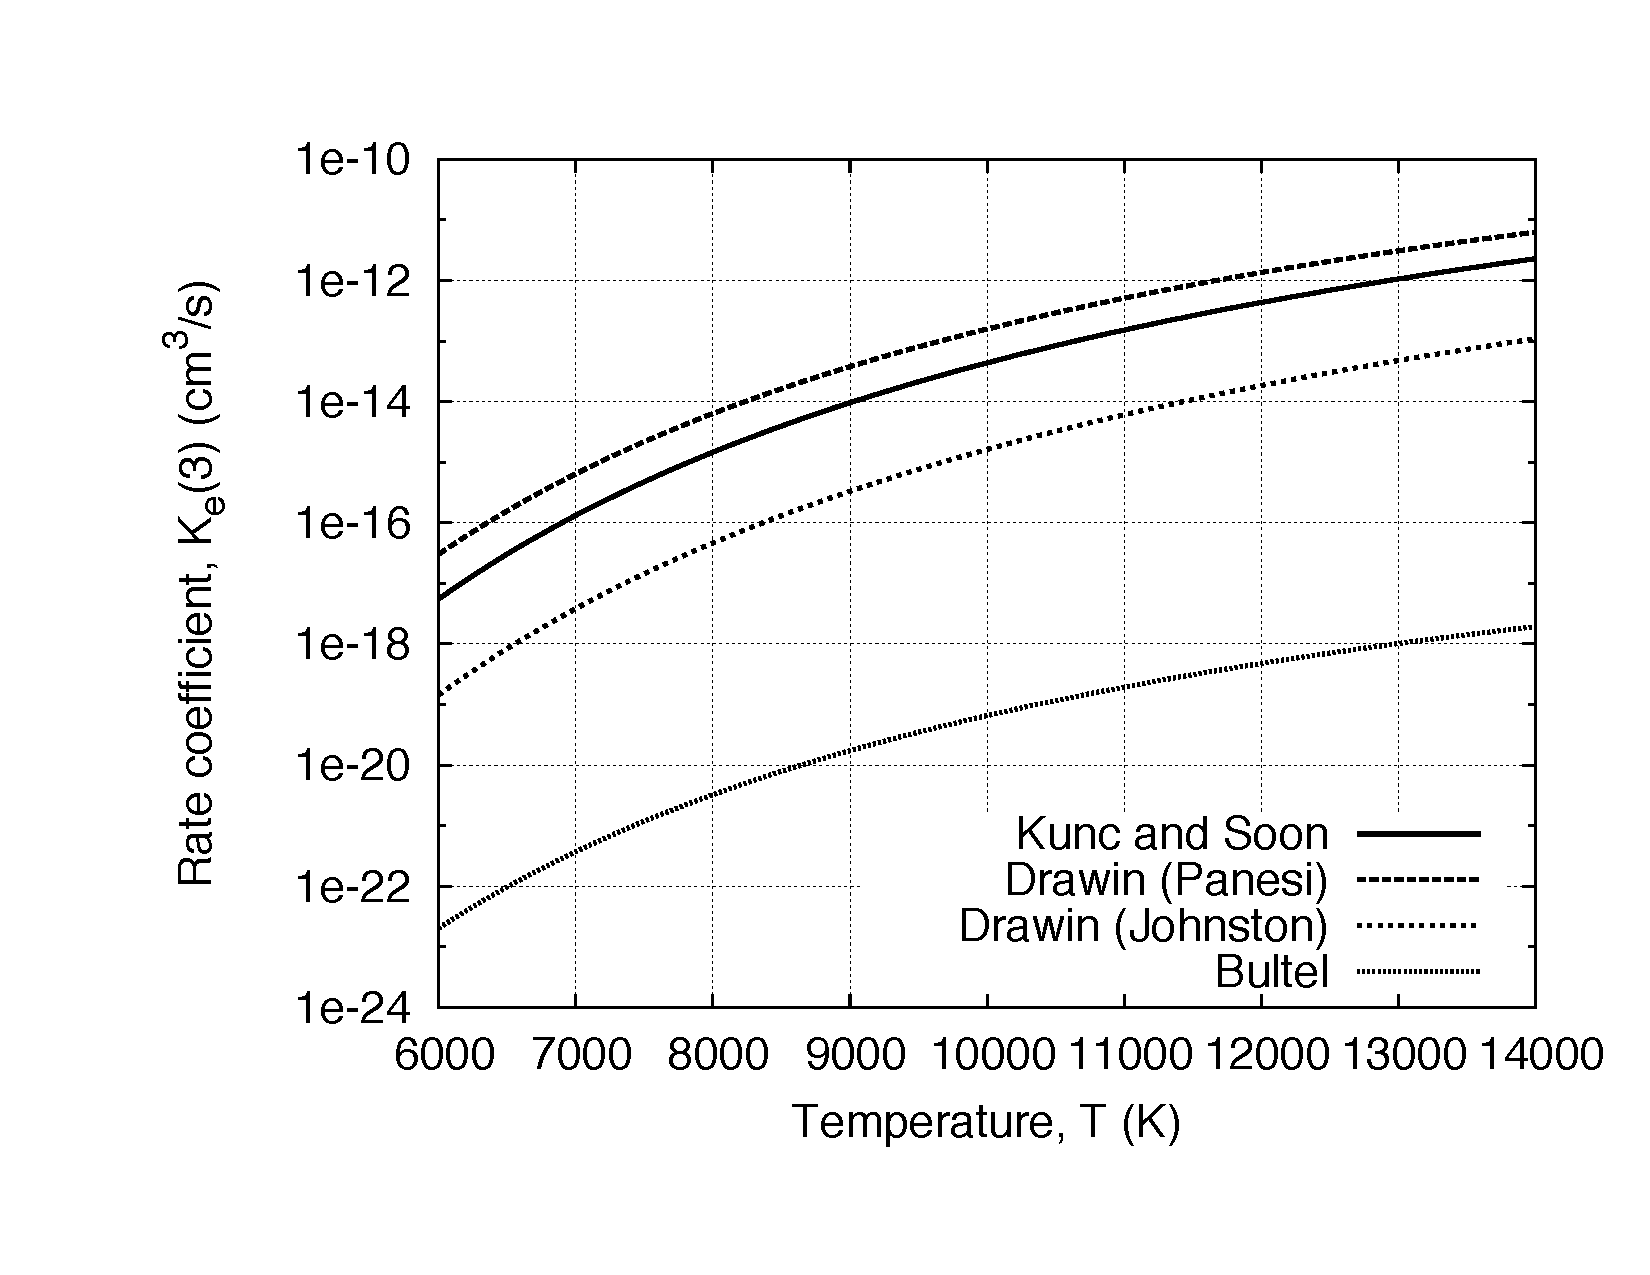
\includegraphics[width=0.48\linewidth]{figures/CR-modelling/K_EII_N_3.pdf} \label{fig:K_EII_N_3}}
 \subfloat[$\text{N } \Nlevthirteen \Rightarrow \text{N}^+$]{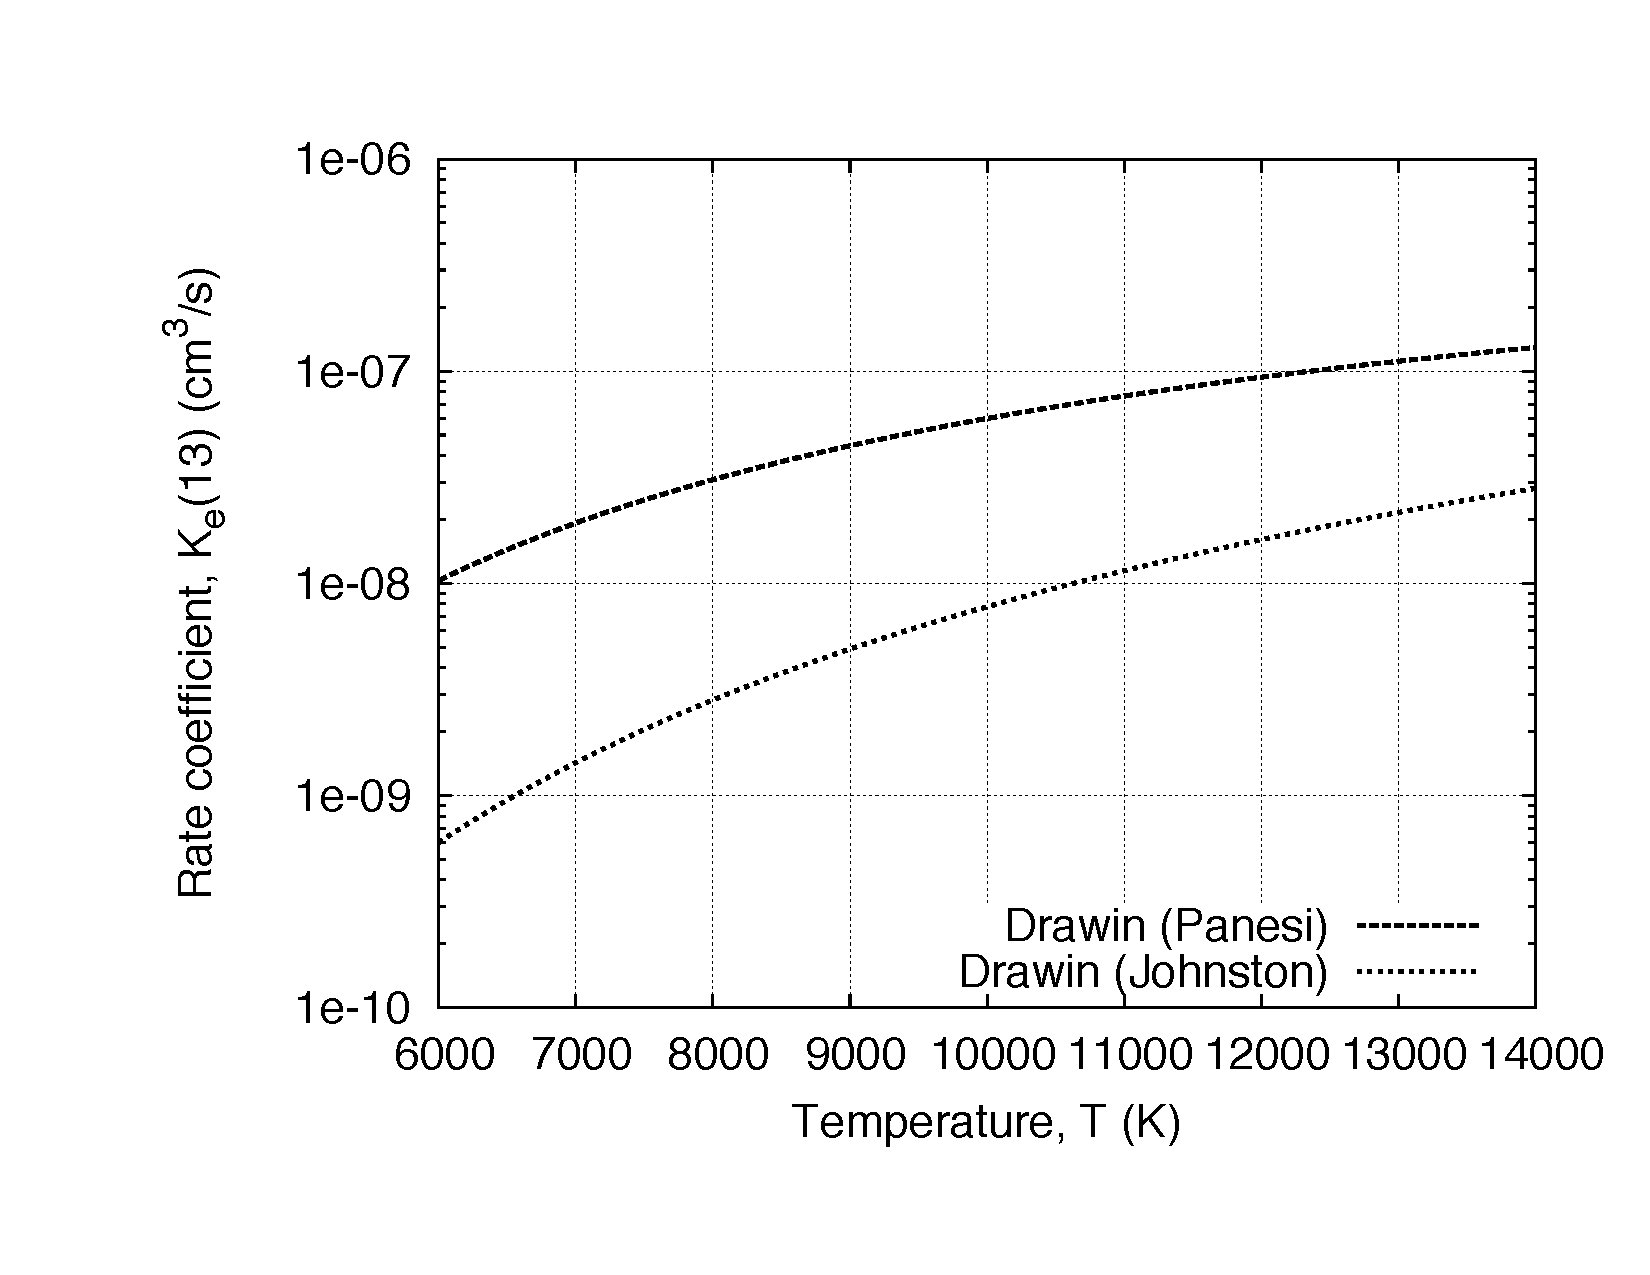
\includegraphics[width=0.48\linewidth]{figures/CR-modelling/K_EII_N_13.pdf} \label{fig:K_EII_N_13}}
 \caption{Comparison of electron impact ionisation rate coefficients for atomic nitrogen.}
 \label{fig:K_EII_N}
\end{figure}

\subsubsection{(a) Electron impact excitation of O}

Zatsarinny and Tayal~\cite{ZT2003} calculated electron impact excitation rates for the ground and first two excited states of atomic oxygen using a $B$-spline $R$-matrix approach.
The forward rate coefficients for the Zatsarinny and Tayal model are calculated as:

\begin{equation}
K_e(i,j) = \frac{8.629 \times 10^{-6}}{g_i \sqrt{T_e}} \gamma_{ij}(T_e) \text{exp} \left ( \frac{-\Delta E_{ij}}{k T_e} \right ) % cm**3 / s
\end{equation}

\noindent where the dimensionless effective collision strength $\gamma_{ij}$ is tabulated as a function of the free electron temperature in Reference~\cite{ZT2003}.
The Zatsarinny and Tayal~\cite{ZT2003} data was the preferred source of accurate atomic oxygen electron impact excitation rates in the collisional-radiative model proposed by Johnston~\cite{JohnPhd}.

\par

Panesi~\cite{panesi_phd} implemented the electron impact excitation rate coefficients presented by Bultel \textit{et al.}~\cite{BBB+2006} which are based on the literature survey of Itikawa and Ichimura~\cite{II1990}.
Electron impact excitation rate coefficients for transitions from the ground state to the two metastable states of atomic oxygen were presented as generalised Arrhenius curve-fits in the temperature range 2,000 $\leq T_e \leq$ 10,000\,K.

\par

Figure~\ref{fig:K_EIE_O} compares the electron impact excitation rate coefficient for various transitions of atomic oxygen for which Zatsarinny and Tayal~\cite{ZT2003} present data.
For the transitions to the metastable states, Figures~\ref{fig:K_EIE_O_1_to_2} and~\ref{fig:K_EIE_O_1_to_3}, the Drawin and Gryzinski models substantially overestimated the theoretical calculations of Zatsarinny and Tayal.
Such a discrepency is to be expected for these inner core transitions due to the hydrogenic assumptions of the Drawin and Gryzinski models.
For the transitions where Bultel rates are available, good agreement is observed with the theoretical calculations of Zatsarinny and Tayal.
Although the $B$-spline $R$-matrix calculations of Zatsarinny and Tayal are bounded by the semi-empirical models for most transitions, for some forbidden transitions such as $2-5$ and $3-7$, Figures~\ref{fig:K_EIE_O_2_to_5} and~\ref{fig:K_EIE_O_3_to_7}, the semi-empirical models underestimate the theoretical rates by at least an order of magnitude for the temperature range considered.
Some some transitions such as 1-16 and 1-17, Figures~\ref{fig:K_EIE_O_1_to_16} and~\ref{fig:K_EIE_O_1_to_17}, the Gryzinski model closely matches the Zatsarinny and Tayal calculations, whilst for others such as 1-20, Figure~\ref{fig:K_EIE_O_1_to_20}, the Drawin model shows exceptional agreement.
The Drawin and Gryzinski models show considerable variability in their relative magnitudes, being within a factor of 2 of each other for some transitions and in excess of $10^4$ for some transitions to high lying states (\textit{e.g.} Figures~\ref{fig:K_EIE_O_1_to_20} and~\ref{fig:K_EIE_O_2_to_20}).
As for atomic nitrogen, we must again bear in mind that Panesi~\cite{panesi_2008B,panesi_phd} found improved agreement with experiment when using the Gryzinski model.
Therefore in the present work the Zatsarinny and Tayal~\cite{ZT2003} rate coefficients are preferred where available, while the Gryzinski~\cite{Gryz59} model is applied to the remaining transitions.

\begin{figure}[p]
 \centering
 \subfloat[$\Olevone \Rightarrow \Olevtwo$ (Forbidden)]{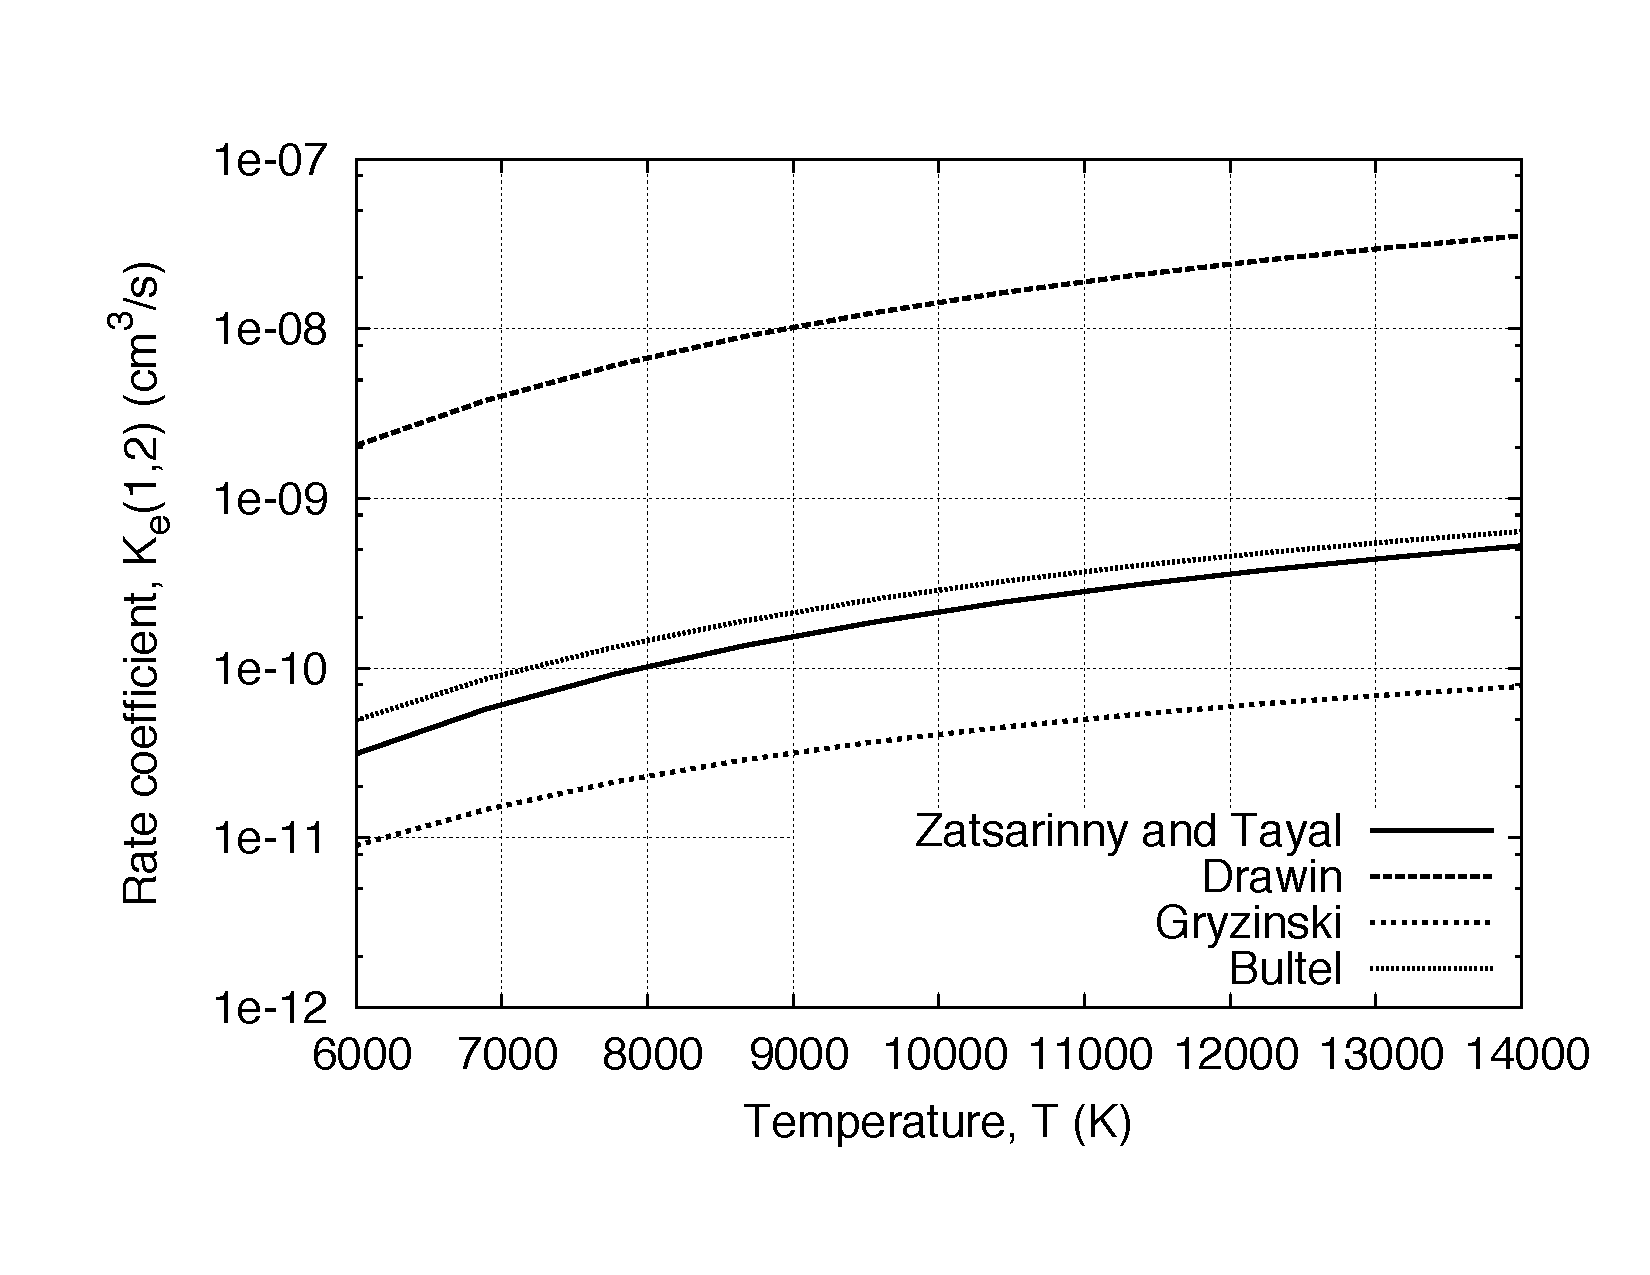
\includegraphics[width=0.48\linewidth]{figures/CR-modelling/K_EIE_O_1_to_2.pdf} \label{fig:K_EIE_O_1_to_2}}
 \subfloat[$\Olevone \Rightarrow \Olevthree$ (Forbidden)]{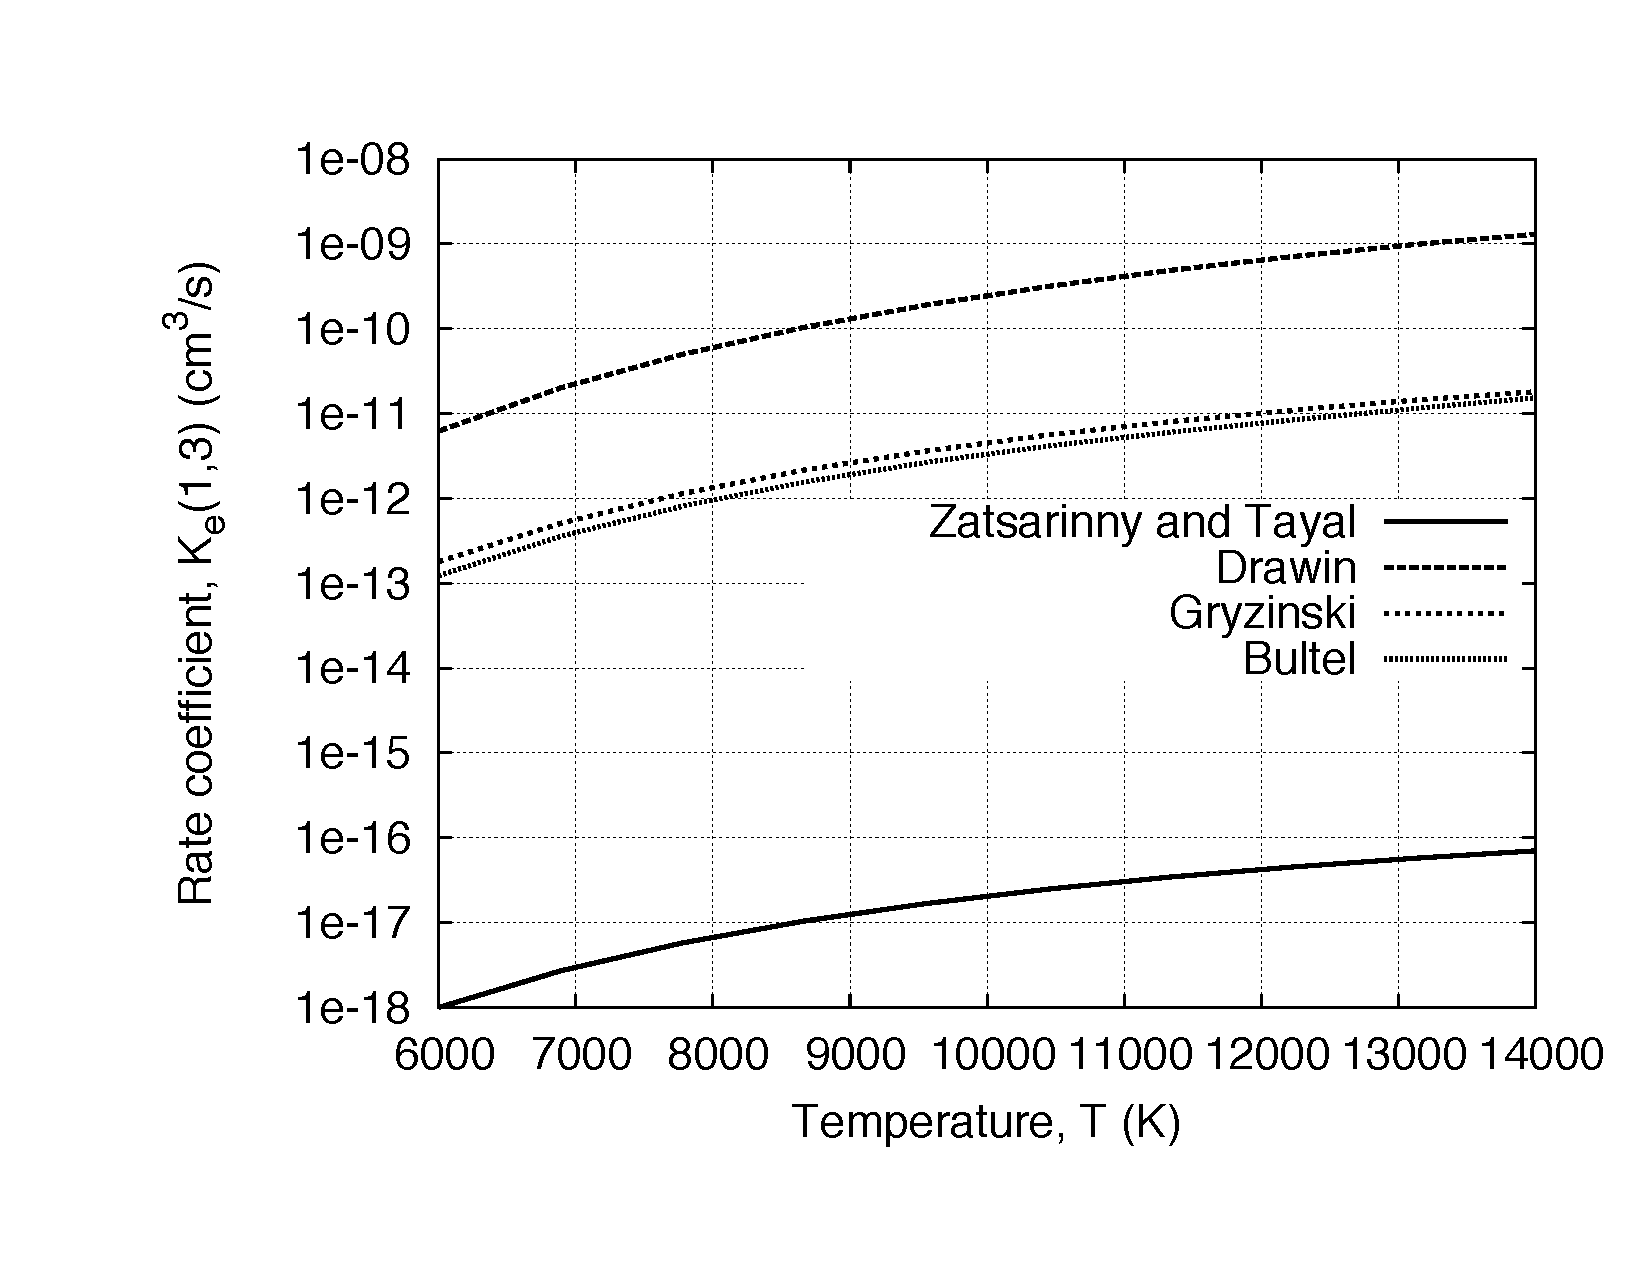
\includegraphics[width=0.48\linewidth]{figures/CR-modelling/K_EIE_O_1_to_3.pdf} \label{fig:K_EIE_O_1_to_3}} \\
 \subfloat[$\Olevone \Rightarrow \Olevfive$ (Allowed)]{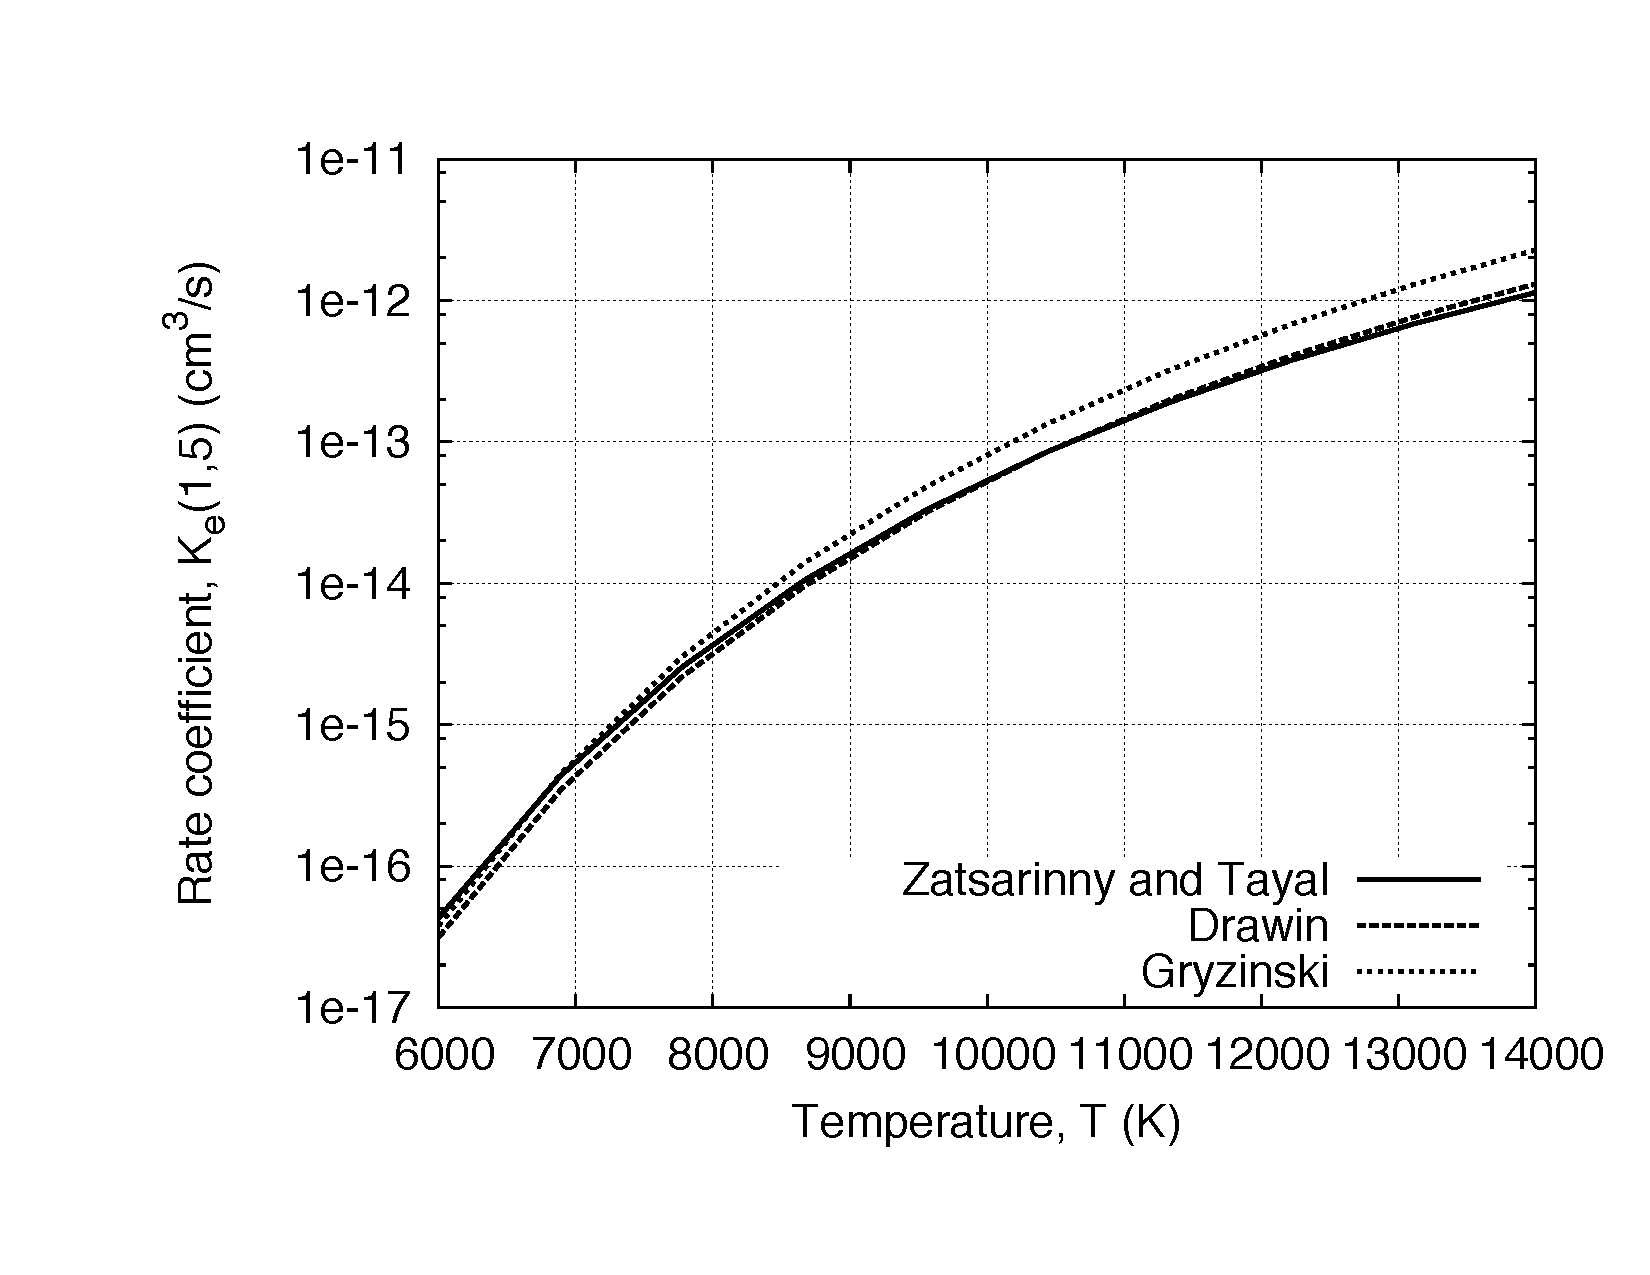
\includegraphics[width=0.48\linewidth]{figures/CR-modelling/K_EIE_O_1_to_5.pdf} \label{fig:K_EIE_O_1_to_5}}
 \subfloat[$\Olevtwo \Rightarrow \Olevfive$ (Forbidden)]{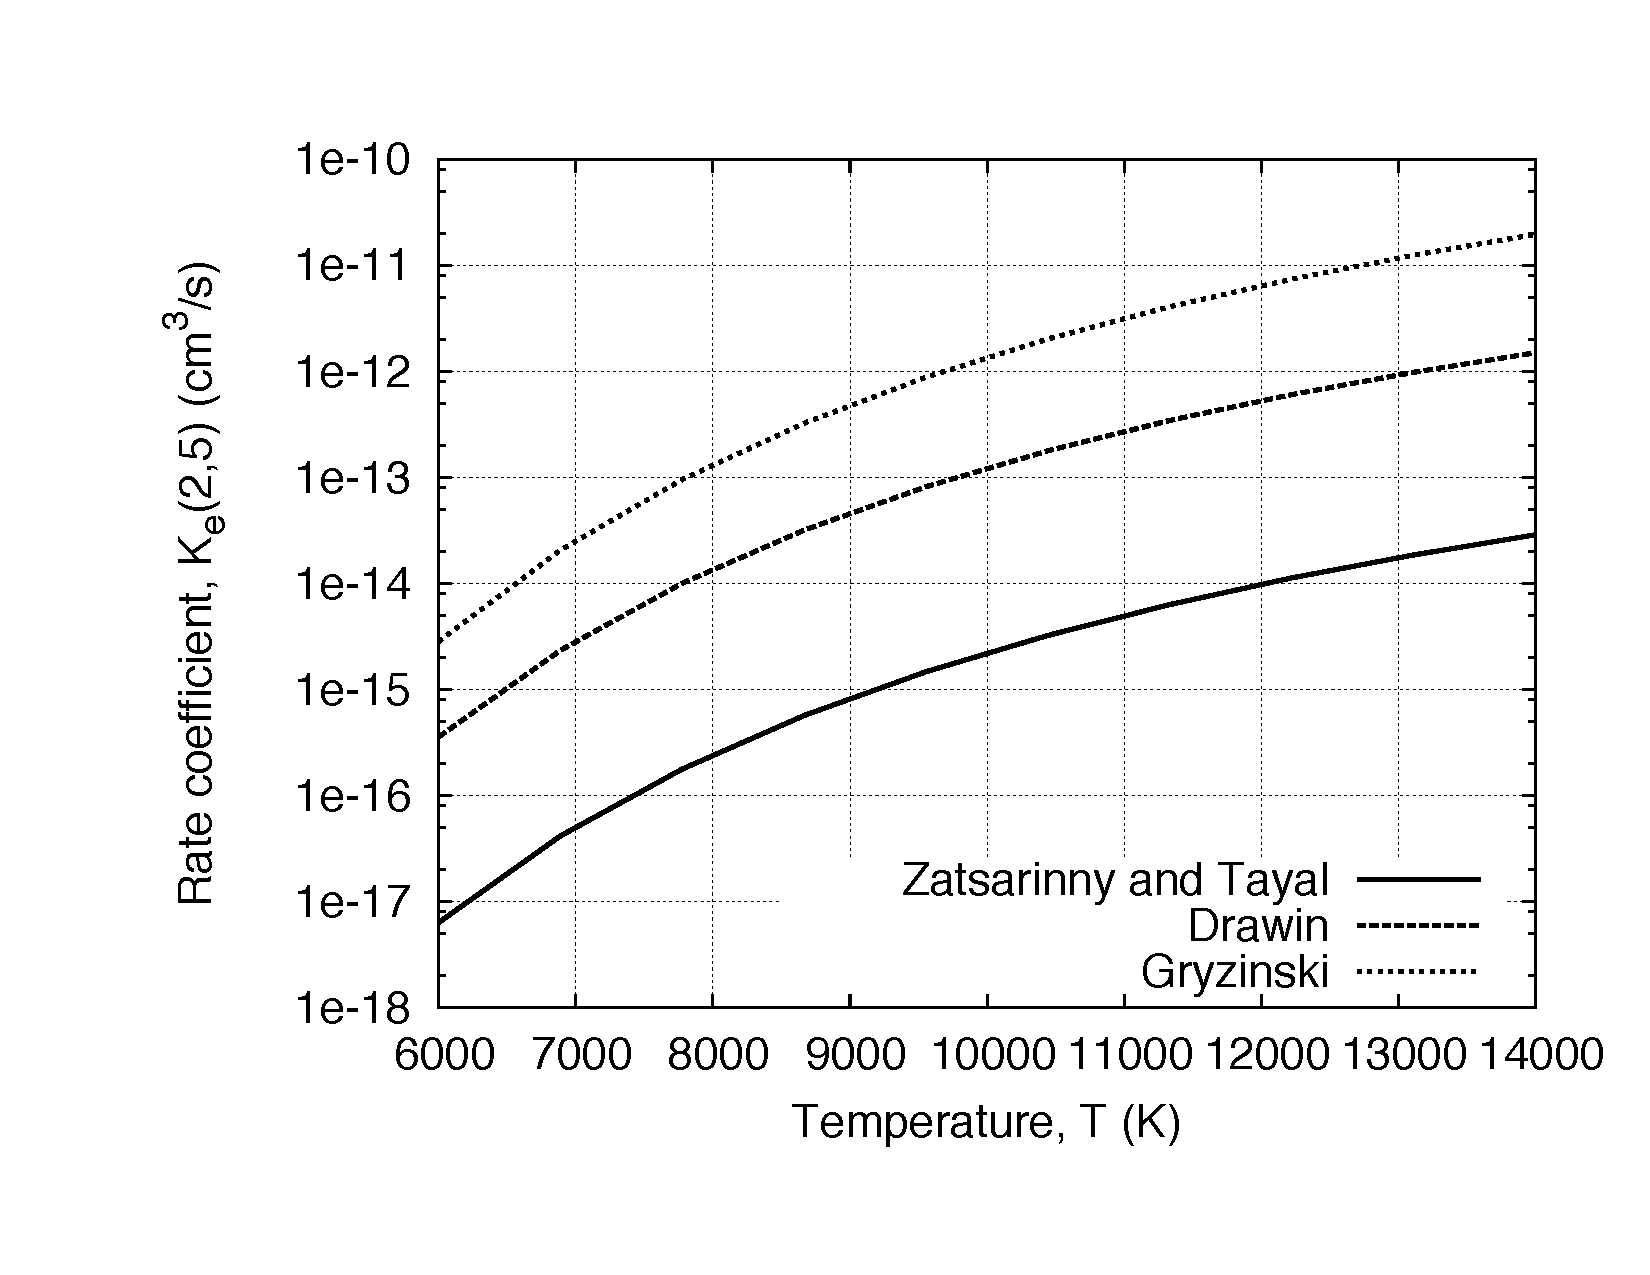
\includegraphics[width=0.48\linewidth]{figures/CR-modelling/K_EIE_O_2_to_5.pdf} \label{fig:K_EIE_O_2_to_5}} \\
 \subfloat[$\Olevone \Rightarrow \Olevten$ (Forbidden)]{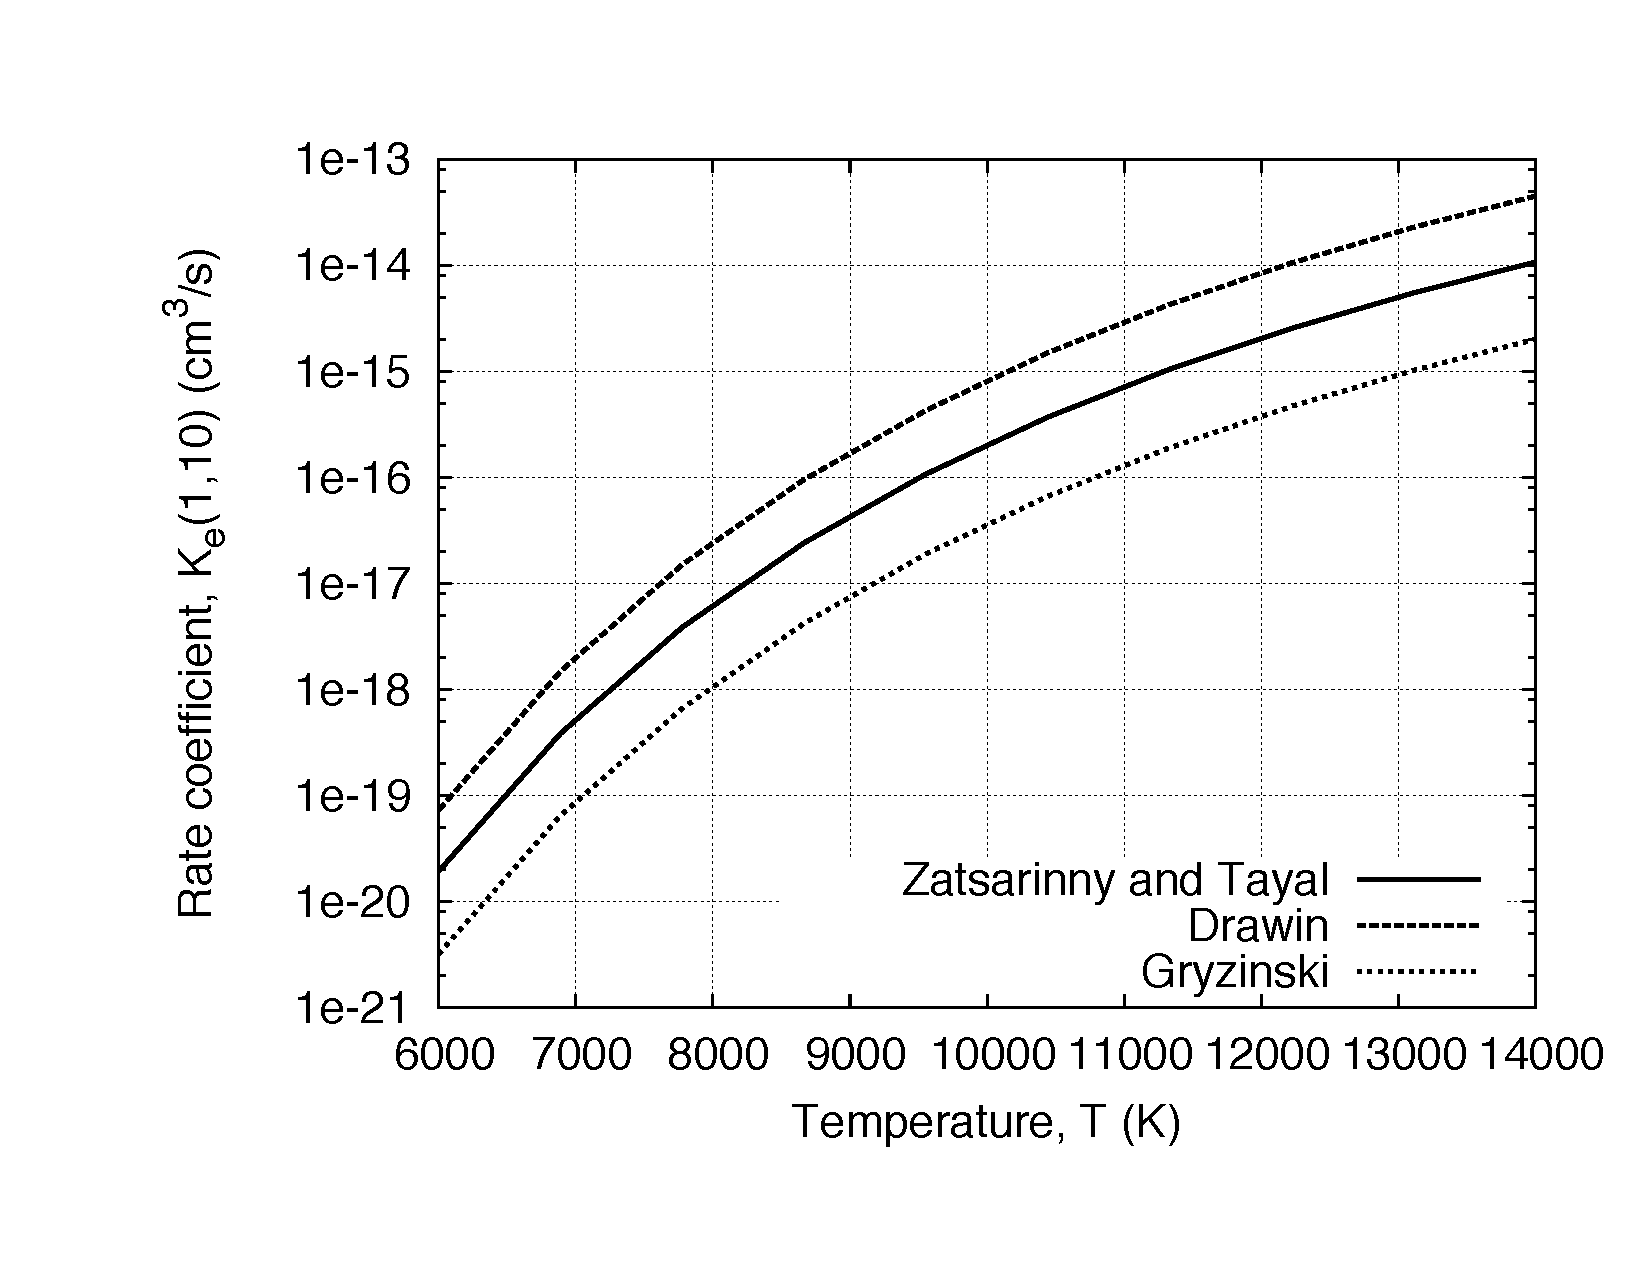
\includegraphics[width=0.48\linewidth]{figures/CR-modelling/K_EIE_O_1_to_10.pdf} \label{fig:K_EIE_O_1_to_10}}
 \subfloat[$\Olevthree \Rightarrow \Olevseven$ (Forbidden)]{\includegraphics[width=0.48\linewidth]{figures/CR-modelling/K_EIE_O_3_to_7.pdf} \label{fig:K_EIE_O_3_to_7}}
 \caption{Comparison of  electron impact excitation rate coefficients for atomic oxygen.}
 \label{fig:K_EIE_O}
\end{figure}
%
\begin{figure}[!hbtp]
 \centering
 \ContinuedFloat
 \subfloat[$\Olevone \Rightarrow \Olevsixteen$ (Allowed)]{\includegraphics[width=0.48\linewidth]{figures/CR-modelling/K_EIE_O_1_to_16.pdf} \label{fig:K_EIE_O_1_to_16}}
 \subfloat[$\Olevone \Rightarrow \Olevseventeen$ (Forbidden)]{\includegraphics[width=0.48\linewidth]{figures/CR-modelling/K_EIE_O_1_to_17.pdf} \label{fig:K_EIE_O_1_to_17}} \\
 \subfloat[$\Olevone \Rightarrow \Olevtwenty$ (Forbidden)]{\includegraphics[width=0.48\linewidth]{figures/CR-modelling/K_EIE_O_1_to_20.pdf} \label{fig:K_EIE_O_1_to_20}}
 \subfloat[$\Olevtwo \Rightarrow \Olevtwenty$ (Forbidden)]{\includegraphics[width=0.48\linewidth]{figures/CR-modelling/K_EIE_O_2_to_20.pdf} \label{fig:K_EIE_O_2_to_20}} \\
 \caption{\textit{(Continued)} Comparison of  electron impact excitation rate coefficients for atomic oxygen.}
 \label{fig:K_EIE_O}
\end{figure}

\subsubsection{Electron impact ionisation of O}

Johnston~\cite{JohnPhd} implemented the ionisation rate coefficients proposed by Soon and Kunc~\cite{SK1990} for the ground and first two excited levels of atomic oxygen.
The rate coefficients are calculated as described in Equations~\ref{eq:K_EII_Soon_Kunc_a} to~\ref{eq:K_EII_Soon_Kunc_c}, where $A=30.52$ and $\chi=4.0$ for levels $i$=1, 2 and 3 of O.
This expression is a curve-fit based on the rate coefficient derived from experimentally measured electron impact ionisation cross sections for the ground state of O.

\par

Panesi~\cite{panesi_phd} implemented the ionisation rate coefficients presented by Bultel \textit{et al.}~\cite{BBB+2006}, which were obtained from the compilation of Tawara and Kato~\cite{TK1999} and the combined binary-encounter Bethe (BEB) and scaled plane-wave Born (PWB) calculations of Kim and Desclaux~\cite{KD2002}.
The rates for the ground and first two excited states of O were presented as generalised Arrhenius curve-fits in the temperature range 2,000 $\leq T_e \leq$ 10,000\,K.

\par

Figure~\ref{fig:K_EII_O} compares the electron impact ionisation rate coefficient for various transitions of O.
The experimentally-fitted Soon and Kunc models and theoretically-fitted Bultel models give excellent agreement for ionisation from the ground state, but exhibit up to an order of magnitude deviation for the $\Olevthree$ multiplet (see Figure~\ref{fig:K_EII_O_3}).
The two Drawin models bound the experimentally fitted model of Kunc and Soon~\cite{KS1989}, with Panesi's implementation being in closer agreement, especially for ionisation of the $\Olevthree$ multiplet.
Similarly as for atomic nitrogen, Johnston's implementation of the Drawin cross sections is between approximately 2 and 100 times smaller than Panesi's implementation for all levels.
Therefore in the present work the electron impact ionisation coefficients of Kunc and Soon~\cite{KS1989} are preferred for the first three levels, while the Drawin model implemented by Panesi~\cite{JohnPhd} is used for the remaining levels.

\begin{figure}[h]
 \centering
 \subfloat[$\text{O } \Olevone \Rightarrow \text{O}^+$]{\includegraphics[width=0.48\linewidth]{figures/CR-modelling/K_EII_O_1.pdf} \label{fig:K_EII_O_1}}
 \subfloat[$\text{O } \Olevtwo \Rightarrow \text{O}^+$]{\includegraphics[width=0.48\linewidth]{figures/CR-modelling/K_EII_O_2.pdf} \label{fig:K_EII_O_2}} \\
 \subfloat[$\text{O } \Olevthree \Rightarrow \text{O}^+$]{\includegraphics[width=0.48\linewidth]{figures/CR-modelling/K_EII_O_3.pdf} \label{fig:K_EII_O_3}}
 \subfloat[$\text{O } \Olevsixteen \Rightarrow \text{O}^+$]{\includegraphics[width=0.48\linewidth]{figures/CR-modelling/K_EII_O_16.pdf} \label{fig:K_EII_O_13}}
 \caption{Comparison of  electron impact ionisation rate coefficients for atomic oxygen.}
 \label{fig:K_EII_O}
\end{figure}

\subsubsection{(b) Diatomic species: N$_2$ and N$_2+$}

Johnston~\cite{JohnPhd} presented collisional-radiative models for N$_2$ and N$_2^+$ compiled from both theoretically calculated and experimentally measured rate-coefficients in the literature.
The majority of the collisional rate coefficients are based on the theoretical calculations of Teulet \textit{et al.}~\cite{TSG1999}, however other more accurate data was preferenced where available.
Since Johnston formulated this model, a set of collisional rate coefficients for the diatomic species CN, CO, N$_2$, N$_2^+$, O$_2$ and NO have been proposed by Park~\cite{park2008a, park2008b}.
The rate coefficients are based on experimentally measured cross sections where available, and theoretically estimated otherwise.

\par

\begin{figure}[t]
 \centering
 \subfloat[$\NNlevX \Longrightarrow \NNlevB$]{\includegraphics[width=0.48\linewidth]{figures/CR-modelling/K_EIE_N2_X_to_B.pdf} \label{fig:K_EIE_N2_X_to_B}}
 \subfloat[$\NNlevA \Longrightarrow \NNlevB$]{\includegraphics[width=0.48\linewidth]{figures/CR-modelling/K_EIE_N2_A_to_B.pdf} \label{fig:K_EIE_N2_A_to_B}}
 \caption{Comparison of electron impact excitation rate coefficients for transitions to the $\NNlevB$ state of N$_2$.}
 \label{fig:K_EIE_N2}
\end{figure}

The most critical reactions for N$_2$ and N$_2^+$ at Earth re-entry conditions are those populating the upper states of radiative transitions via electron impact excitation.
Figure~\ref{fig:K_EIE_N2} compares the electron impact excitation rates populating the $\NNlevB$ state of N$_2$ (upper state for the First Positive band system), and Figure~\ref{fig:K_EIE_N2_plus} compares the electron impact excitation rates populating the $\NNplevB$ state of N$_2^+$ (upper state for the First Negative band system).
While the two models agree to within a factor of 4 for the \PIEreac{N$_2$}{e$^-$}{\NNlevX}{\NNlevB} transition, Figure~\ref{fig:K_EIE_N2_X_to_B}, the Park rates are substantially higher than those of Johnston for the other transitions.
For the \PIEreac{N$_2$}{e$^-$}{\NNplevA}{\NNplevB} transition in Figure~\ref{fig:K_EIE_N2_plus_A_to_B}, for example, the Park rate is almost four orders of magnitude greater than the Johnston rate.
Although not shown here, the estimated rate of Teulet \textit{et al.}~\cite{TSG1999} for the \PIEreac{N$_2^+$}{e$^-$}{\NNplevX}{\NNplevB} transition is quite similar to the Park rate.
In Johnston's~\cite{JohnPhd} survey of the literature, this rate of Teulet was found to overestimate those from more accurate theoretical calculations.
Furthermore, in Reference~\cite{CJ_EAST_2008} the rates of Teulet were required to be reduced by factors of 10 and 70 for N$_2$ and N$_2^+$ respectively in order to achieve agreement with experiment.
In the present work therefore we choose to adopt the Johnston~\cite{JohnPhd} model.
The collisional-radiative models for N$_2$ and N$_2^+$ are summarised in \textsection~\ref{sec:N2_CR} and~\ref{sec:N2p_CR} respectively.
The nonequilibrium levels considered for N$_2$ are $\NNlevX$, $\NNlevA$, $\NNlevB$ and $\NNlevC$, while those for N$_2^+$ are $\NNplevX$, $\NNplevA$, $\NNplevB$ and $\NNplevC$.

\begin{figure}[h!]
 \centering
 \subfloat[$\NNplevX \Longrightarrow \NNplevB$]{\includegraphics[width=0.48\linewidth]{figures/CR-modelling/K_EIE_N2_plus_X_to_B.pdf} \label{fig:K_EIE_N2_plus_X_to_B}}
 \subfloat[$\NNplevA \Longrightarrow \NNplevB$]{\includegraphics[width=0.48\linewidth]{figures/CR-modelling/K_EIE_N2_plus_A_to_B.pdf} \label{fig:K_EIE_N2_plus_A_to_B}}
 \caption{Comparison of electron impact excitation rate coefficients for transitions to the $\NNplevB$ state of N$_2^+$.}
 \label{fig:K_EIE_N2_plus}
\end{figure}

\FloatBarrier

\subsection{Collisional-radiative model for CO$_2$--N$_2$--Ar mixtures}

 \begin{figure}[p]
 \centering
 \subfloat[Number density profile]{\includegraphics[width=0.9\linewidth]{figures/CR-modelling/Mars_number_densities.pdf} \label{fig:Mars_number_densities}} \\
 \subfloat[Radiative emission profile]{\includegraphics[width=0.9\linewidth]{figures/CR-modelling/Mars_emissions.pdf} \label{fig:Mars_emissions}}
 \caption{Post-shock species number density and radiative emission profiles along the stagnation streamline for a hypothetical Mars aerocapture entry condition ($p_\infty = 6.2$\,Pa, $T_\infty = 161$\,K, $u_\infty = 9,440$\,m/s).}
\end{figure}

Figures~\ref{fig:Mars_number_densities} and~\ref{fig:Mars_emissions} present post-shock species number density and radiative emission profiles respectively for a hypothetical high-speed Mars aerocapture condition from the trajectory study of Braun \textit{et al.}~\cite{BPH90}.
The condition corresponds to that predicted for an aerocapture vehicle with nose radius 10\,m at 44.9\,km altitude that entered the Martian atmosphere at 9.79\,km/s.
This point is just prior to peak heating and is characterised by very strong thermochemical nonequilibrium.
Behind the shock CO$_2$ and N$_2$ quickly dissociate, forming an initial pool of CO and N$_2$ molecules and C, N and O atoms that allow exchange reactions to begin.
At 1\,mm behind the shock reactions have only just begun to occur and CN and C$_2$ systems and continuum transitions dominate the radiative emission.
By 3\,mm behind the shock dissociation is essentially complete and peak emission occurs, with atomic C lines, the VUV CO band systems and atomic O lines contributing 99\% of the radiative emission.
At peak emission the next strongest radiators are N, CN, C$_2$ and Ar, however their emission strength is on average two orders of magnitude less than CO and C.
As equilibrium is approached the total radiation drops by an order of magnitude, C, CO and O (in that order) continue to dominate the radiative emission while the relative strength of the continuum transitions increases due to the growing free electron population.
The free electron mole-fraction between peak-emission and chemical equilibrium is in the order of $10^{-2}$.

\par

Although C, CO and O are by far the strongest radiators when Boltzmann level populations is assumed, the nonequilibrium emission is likely to be significantly less due to radiative depletion of the high lying states.  
Therefore in the present work we chose to apply the collisional-radiative model to all the significant radiators -- C, CO, O, C$_2$, N, Ar and CN.
Although the free electron number density is lower than for Earth re-entry, electron impact collisional processes should still dominate over heavy particle collisions due to their high efficiency.
Thus in the present work only electron impact collisional processes will be considered.

\subsubsection{Atomic species: Ar, C, N and O}

Table~\ref{tab:Ar-C-N-O-CR} summarises the implemented rate coefficients for the collisional-radiative mechanisms considered for atomic species in CO$_2$--N$_2$--Ar mixtures.
Similarly as for N$_2$--O$_2$ mixtures, the collisional mechanisms considered for atoms are electron impact excitation and ionisation, and the radiative processes considered are bound-bound optically allowed transitions.
As the Drawin~\cite{drawin_1968} cross sections have been shown to be appropriate for calculating non-Boltzmann emission from atomic argon~\cite{Vlcek1989, BGV1998}, the Drawin model proposed by Panesi~\cite{panesi_phd} is applied to calculate electron impact excitation and ionisation of Ar.
For atomic carbon, accurate rate-coefficients are obtained from Suno and Kato~\cite{SK2006} for electron impact excitation and ionisation of the ground and metastable states.
The remaining transitions described by the semi-empirical model of Gryzinski~\cite{Gryz59}.
The collisional-radiative models selected for N and O in N$_2$--O$_2$ mixtures are retained here for application to CO$_2$--N$_2$--Ar mixtures.
All radiative transition probabilities $A(i,j)$ are calculated using Equation~\ref{eq:A_av} where the individual line transition probabilities are obtained from the NIST Atomic Species Database~\cite{NIST_ASD} (see Table~\ref{tab:atomic-lines}).

\begin{table}[bht]
 \center
 \caption{Summary of the collisional-radiative mechanisms implemented for Ar, C, N and O in CO$_2$--N$_2$--Ar mixtures.}
 \label{tab:Ar-C-N-O-CR}
 \begin{tabular*}{1.0\textwidth}{cccc}
  \hline Species                         & Electronic levels & CR mechanisms                                & Models    \\
  \hline  
                  Ar                               & All & Electron impact excitation                & Drawin (Reference~\cite{panesi_phd}) \\
                                                     &       & Electron impact ionisation               &  Drawin (Reference~\cite{panesi_phd}) \\
                                                     &       & Radiative decay                                 & NIST Atomic Spectra Database~\cite{NIST_ASD} \\
                  C                                & All & Electron impact excitation                & (a) Suno and Kato~\cite{SK2006} \\
                                                     &       &                                                               & (b) Gryzinski~\cite{Gryz59} \\
                                                     &       & Electron impact ionisation               & (a) Suno and Kato~\cite{SK2006} \\
                                                     &       &                                                               & (b) Drawin (Reference~\cite{panesi_phd}) \\
                                                     &       & Radiative decay                                 & NIST Atomic Spectra Database~\cite{NIST_ASD} \\    
                  N                                & All & Electron impact excitation                & (a) Frost \textit{et al.}~\cite{FAS+1998} \\
                                                     &       &                                                               & (b) Gryzinski~\cite{Gryz59} \\
                                                     &       & Electron impact ionisation               & (a) Soon and Kunc~\cite{SK1990} \\
                                                     &       &                                                               & (b) Drawin (Reference~\cite{panesi_phd}) \\
                                                     &       & Radiative decay                                 & NIST Atomic Spectra Database~\cite{NIST_ASD} \\
                  O                                & All & Electron impact excitation                & (a) Zatsarinny and Tayal~\cite{ZT2003} \\
                                                     &       &                                                               & (b) Gryzinski~\cite{Gryz59} \\
                                                     &       & Electron impact ionisation               & (a) Soon and Kunc~\cite{SK1990} \\
                                                     &       &                                                               & (b) Drawin (Reference~\cite{panesi_phd}) \\
                                                     &       & Radiative decay                                 & NIST Atomic Spectra Database~\cite{NIST_ASD} \\                                   
  \hline
 \end{tabular*}
\end{table}


\subsubsection{(a) Electron impact excitation of C}


Suno and Kato~\cite{SK2006} compiled an extensive electron-impact ionisation, excitation and charge exchange cross section database for carbon atoms and ions.
Although the database extends to electron temperatures of 1\,keV as it is designed nuclear fusion applications, the presented electron impact excitation data for C is shown to agree well with the experimental data of Duneath \textit{et al.}~\cite{DFB+1997} and others obtained in the 1\,eV electron temperature range of present interest.
The data are presented as curve fits for the collision strength $\Omega_{ij}$ from which the rate coefficient can be calculated as:

\begin{equation}
 K_e(i,j) = \frac{8.010 \times 10^{-8}}{\omega_i \sqrt{T_e}} y \int_1^\infty \Omega_{ij} e^{-y X} dX 
\end{equation}

\noindent where $T_e$ is in eV, $y = \Delta E_{ij} / T_e$ and $X = E_e / \Delta E_{ij}$.

\par

Figure~\ref{fig:K_EIE_C} compares the electron impact excitation rate coefficient for various transitions of C.
For all transitions except excitation of the ground to first excited state (see Figure~\ref{fig:K_EIE_C_1_to_2}}), the Suno and Kato rates are between 2 and 1000 times larger than the rates predicted by the approximate models.
This is in contrast to the electron impact excitation rates of N and O, where the accurate rates for low lying levels was bounded by the approximate models.
It is therefore possible that the rates of Suno and Kato are not suitable for the temperature range considered.
In the absence of better electron impact excitation data, however, the Suno and Kato rates are preferenced for transitions from low lying states while the Gryzinski model is applied to the remaining transitions.

\begin{figure}[p]
 \centering
 \subfloat[$\Clevone \Rightarrow \Clevtwo$ (Forbidden)]{\includegraphics[width=0.48\linewidth]{figures/CR-modelling/K_EIE_C_1_to_2.pdf} \label{fig:K_EIE_C_1_to_2}}
 \subfloat[$\Clevtwo \Rightarrow \Clevthree$ (Forbidden)]{\includegraphics[width=0.48\linewidth]{figures/CR-modelling/K_EIE_C_2_to_3.pdf} \label{fig:K_EIE_C_2_to_3}} \\
 \subfloat[$\Clevone \Rightarrow \Clevfive$ (Allowed)]{\includegraphics[width=0.48\linewidth]{figures/CR-modelling/K_EIE_C_1_to_5.pdf} \label{fig:K_EIE_C_1_to_5}}
 \subfloat[$\Clevtwo \Rightarrow \Clevfive$ (Forbidden)]{\includegraphics[width=0.48\linewidth]{figures/CR-modelling/K_EIE_C_2_to_5.pdf} \label{fig:K_EIE_C_2_to_5}} \\
 \subfloat[$\Clevone \Rightarrow \Clevfifteen$ (Forbidden)]{\includegraphics[width=0.48\linewidth]{figures/CR-modelling/K_EIE_C_1_to_15.pdf} \label{fig:K_EIE_C_1_to_15}}
 \subfloat[$\Clevone \Rightarrow \Cleveighteen$ (Allowed)]{\includegraphics[width=0.48\linewidth]{figures/CR-modelling/K_EIE_C_1_to_18.pdf} \label{fig:K_EIE_C_1_to_18}}
 \caption{Comparison of  electron impact excitation rate coefficients for atomic carbon.}
 \label{fig:K_EIE_O}
\end{figure}
%
\begin{figure}[!t]
 \centering
 \ContinuedFloat
  \subfloat[$\Clevone \Rightarrow \Clevtwenty$ (Forbidden)]{\includegraphics[width=0.48\linewidth]{figures/CR-modelling/K_EIE_C_1_to_20.pdf} \label{fig:K_EIE_C_1_to_20}} 
  \subfloat[$\Clevone \Rightarrow \Clevtwentytwo$ (Allowed)]{\includegraphics[width=0.48\linewidth]{figures/CR-modelling/K_EIE_C_1_to_22.pdf} \label{fig:K_EIE_C_1_to_22}} 
 \caption{\textit{(Continued)} Comparison of  electron impact excitation rate coefficients for atomic carbon.}
 \label{fig:K_EIE_C}
\end{figure}

\subsubsection{(b) Electron impact ionisation of C}

Suno and Kato~\cite{SK2006} present the electron impact ionisation cross section for the ground state of atomic carbon in the following form:

\begin{equation}
 \sigma = \frac{1 \times 10^{-13}}{I E} \left \lbrace A_1 \text{ln} \left ( E / I \right ) + \sum_{j=2}^{N_A} A_j \left ( 1 - \frac{I}{E} \right )^{j-1} \right \rbrace \label{eq:SK_EII_CS}
\end{equation}

\noindent where $I$ and $E$ are the ionisation and electron energy in eV and $A_j$ are fitting coefficients.
The fitting coefficients have been selected to match the experimental measurements of Brook \textit{et al.}~\cite{BHS1978}.
Unfortunately Brook considered electron energies in the range $ 7 \leq E \leq 1000$\,eV, which is outside the $E \approx 1$\,eV range of present interest.
In the absence of electron impact ionisation cross sections for the metastable state of atomic carbon, in the present work Equation~\ref{eq:SK_EII_CS} is applied where $I$ is taken as the level-specific ionisation potential.
The rate coefficient is then calculated as:

\begin{equation}
 K_e(i,c) = \frac{8.010 \times 10^{-8}}{g_i \sqrt{T_e}} y \int_1^\infty \Omega_i e^{-y X} dX 
\end{equation}

\noindent where $T_e$ is in eV, $y = I / T_e$, $X = E_e / I$ and collision strength $\Omega_i$ for level $i$ is obtained from the cross section in Equation~\ref{eq:SK_EII_CS} via:

\begin{equation}
 \Omega_i = \sigma_{i} \frac{g_i E}{1.1969 \times 10^{-15}}   
\end{equation}

\par

Figure~\ref{fig:K_EII_C} compares the electron impact ionisation rate coefficient for various transitions of C.
The bulk atomic carbon ionisation rate proposed by Park~\cite{park_1994} is overlaid in Figure~\ref{fig:K_EII_C_1} for comparison with the ground state rates.
The Suno and Kato rates are approximately three orders of magnitude greater than the semi-empirical models, and is similar to the Park rate for the ground state.
Similarly as for atomic nitrogen and oxygen, Johnston's implementation of the Drawin cross sections is between approximately 2 and 100 times smaller than Panesi's implementation for all levels.
Therefore in the present work the electron impact ionisation coefficients of Suno and Kato ~\cite{SK2006} are preferred for the first three levels, while the Drawin model implemented by Panesi~\cite{JohnPhd} is used for the remaining levels.

\begin{figure}[h]
 \centering
 \subfloat[$\text{C } \Clevone \Rightarrow \text{C}^+$]{\includegraphics[width=0.48\linewidth]{figures/CR-modelling/K_EII_C_1.pdf} \label{fig:K_EII_C_1}}
 \subfloat[$\text{C } \Clevtwo \Rightarrow \text{C}^+$]{\includegraphics[width=0.48\linewidth]{figures/CR-modelling/K_EII_C_2.pdf} \label{fig:K_EII_C_2}} \\
 \subfloat[$\text{C } \Clevthree \Rightarrow \text{C}^+$]{\includegraphics[width=0.48\linewidth]{figures/CR-modelling/K_EII_C_3.pdf} \label{fig:K_EII_C_3}}
 \subfloat[$\text{C } \Clevfifteen \Rightarrow \text{C}^+$]{\includegraphics[width=0.48\linewidth]{figures/CR-modelling/K_EII_C_15.pdf} \label{fig:K_EII_C_15}}
 \caption{Comparison of  electron impact ionisation rate coefficients for atomic carbon.}
 \label{fig:K_EII_C}
\end{figure}

\subsubsection{Diatomic species: C$_2$, CN and CO}

Zalogin~\cite{zalogin_2001} proposed a simple collisional-radiative model for C$_2$, CN and CO.
This model was `tuned' to match the intensity profiles measured for a 3.45\,km/s CO$_2$--N$_2$ shock tube condition, and was applied with limited success to the 8.5\,km/s CO$_2$--N$_2$ EAST shock tube condition in Reference~\cite{potter_2008c}.
Since this model was formulated, however, a set of collisional-rate coefficients and cross sections for the diatomic species CN, CO, N$_2$, N$_2^+$, O$_2$ and NO have been proposed by Park~\cite{park2008a, park2008b}.
Figure~\ref{fig:K_Park_v_Zalogin} compares the rates that are given by both Zalogin~\cite{zalogin_2001} and Park~\cite{park2008a, park2008b}.
The Zalogin model predicts faster collisional excitation of CN and slower collisional excitation of CO.
%Due to large differences between some of the rates both models were assessed via comparison with shock tube data in~\cite{Potter_PhD}.
As the Park model is more comprehensive and based on experimental and theoretical cross sections where possible, the Park collisional excitation rates for CO and CN are tentatively accepted for inclusion in the nominal collisional-radiative models for these species.
Due to numerical difficulties encountered when implementing the heavy particle impact rates given in Reference \cite{park2008b}, however, these were omitted for CO and CN.
Considering just the electron impact processes should be sufficient for the conditions of interest due to the substantial levels of ionisation.
It should be emphasised that the heavy particle impact processes would need to be considered for the collisional-radiative model to be valid for less energetic conditions where ionisation levels are low.
The system radiative transition probabilities are calculated from the electronic-vibration transition moments via Equation~\ref{eq:A_av_diatomic}.
For C$_2$ we resort to the Zalogin~\cite{zalogin_2001} model as this species was not considered by Park in References~\cite{park2008a, park2008b}.
The nominal collisional-radiative models for C$_2$, CN and CO are summarised in \textsection~\ref{sec:C2_CR} to~\ref{sec:CO_CR} respectively.


\begin{figure}[h]
 \centering
 \subfloat[$\text{CN } \CNlevX + \text{e}^- \Longrightarrow \text{CN }\CNlevA + \text{e}^-$]{\includegraphics[width=0.48\linewidth]{figures/CR-modelling/K_EIE_CN_X_to_A.pdf} \label{fig:K_EIE_CN_X_to_A}}
 \subfloat[$\text{CN }\CNlevX + \text{e}^- \Longrightarrow \text{CN }\CNlevB + \text{e}^-$]{\includegraphics[width=0.48\linewidth]{figures/CR-modelling/K_EIE_CN_X_to_B.pdf} \label{fig:K_EIE_CN_X_to_B}} \\
 \subfloat[$\text{CN }\CNlevX + \text{M}   \Longrightarrow \text{CN }\CNlevA + \text{M}$  ]{\includegraphics[width=0.48\linewidth]{figures/CR-modelling/K_HPIE_CN_X_to_A.pdf} \label{fig:K_HPIE_CN_X_to_A}}
 \subfloat[$\text{CO }\COlevX + \text{e}^- \Longrightarrow \text{CO }\COlevA + \text{e}^- $]{\includegraphics[width=0.48\linewidth]{figures/CR-modelling/K_EIE_CO_X_to_A.pdf} \label{fig:K_EIE_CO_X_to_A}}
 \caption{Comparison of excitation rate coefficients obtained from Park~\cite{park2008a,park2008b} and Zalogin~\cite{zalogin_2001}.}
 \label{fig:K_Park_v_Zalogin}
\end{figure}

\subsection{A note on the selection of data sources}

In formulating the collisional-radiative model the sometimes contradictory issues of data source consistency and model accuracy arise.
On one hand, it is desirable to formulate a model that is both internally consistent (uses the same data source for all processes) and externally consistent (uses the same data sources as other models, such as the spectral radiation model).
On the other hand, it is desirable to formulate a model that best reproduces the physical phenomena.
The goal of the present work is to develop effective engineering tools, and therefore the latter approach has been preferenced to give the calculations the best chance of reproducing experimental data.
As an example, consider the electron impact excitation for the nitrogen atom.
An internally consistent model would have to use an empirical model such as that of Drawin~\cite{drawin_1968} for all transitions, however this model has been shown to give inaccurate results when applied to the excitation of low lying electronic states~\cite{panesi_2008B,panesi_phd}.
Although it breaks the internal consistency of the model, implementing the computational chemistry rates of Frost \textit{et al.}~\cite{FAS+1998} gives much improved comparisons with experiment~\cite{panesi_2008B,panesi_phd}.
This principal of selecting the most effective data, rather than the most consistent data, has been applied throughout the collisional-radiative model.


